% Results and Evaluation

\chapter{نتایج و ارزیابی}\label{ch:5}
\section{مقدمه}\label{sec:5:1}
در این فصل دو روش \lr{KNN-LSTSVM} و \lr{RKNN-TSVM} به ترتیب در بخش‌های ‏\ref{sec:5:2} و ‏\ref{sec:5:3} به صورت جامع بررسی و ارزیابی می‌شود. این روش‌ها در دو بخش جداگانه مورد بررسی قرار گرفته‌اند. زیرا ایده و هدف اصلی این دو روش با یکدیگر متفاوت است. 
\begin{enumerate}
	\item هدف اصلی در روش \lr{KNN-LSTSVM} ضمن حفظ مزیت اصلی روش \lr{LSTSVM}، اضافه کردن گراف نزدیک‌ترین همسایه به منظور بهبود دقت این مدل است.
	\item 	روش \lr{RKNN-TSVM} با کمینه کردن ریسک ساختاری و شیوه جدید وزن‌دهی، دقت روش \lr{WLTSVM} را بهبود می‌دهد. با این حال در روش \lr{RKNN-TSVM}، افزایش سرعت آموزش هم مد نظر است.
\end{enumerate}

در ادامه عملکرد دو دسته‌بند پیشنهادی از نظر دقت و سرعت روی مجموعه داده‌های مختلف سنجیده می‌شود.

\section{ارزیابی روش \lr{KNN-LSTSVM}}\label{sec:5:2}
ابتدا نحوه پیاده‌سازی و انتخاب پارامترهای بهینه توضیح داده شده است. سپس عملکرد روش \lr{KNN-LSTSVM} روی مجموعه داده‌های مصنوعی بررسی می‌شود. بطوریکه ناحیه تصمیم خطی و غیر خطی این روش در فضای دو بعدی نشان داده شده است. در آخر نتایج روی مجموعه داده‌های \lr{UCI} و \lr{NDC} مورد بحث قرار می‌گیرد.

\subsection{نحوه پیاده‌سازی و اجرای الگوریتم‌ها}\label{sec:5:2:1}
تمام روش‌ها در زبان برنامه‌نویسی پایتون\LTRfootnote{\lr{Python}}  \cite{ceder2010} پیاده‌سازی شده است. آزمایش‌ها روی یک کامپیوتر شخصی با پردازنده \lr{Core i7 6700K}، سیستم عامل \lr{Windows 8} و 32 گیگابایت حافظه صورت گرفته است. اعمال جبر خطی با کتابخانه \lr{NumPy} \cite{walt2011} انجام شده است. همچنین کتابخانه \lr{SciPy} \cite{jones2014} برای محاسبه فاصله و توابع آماری بکار گرفته شده است. همچنین الگوریتم بهینه‌سازی \lr{clipDCD} جهت بهبود سرعت اجرا، در \lr{Cython} \cite{behnel2011} پیاده‌سازی شده است.

دقت روش \lr{TSVM} و گسترش‌هایش به انتخاب پارامترهای بهینه بسیار وابسته است. بدین منظور \gls{GS}  برای پیدا کردن پارامترهای بهینه استفاده می‌شود. همچنین تابع \lr{TSVM} را به عنوان تابع هسته  $k(x_i, x_j)=\exp({-\left\|x_i - x_j\right\|^2}/\gamma^2)$ اغلب بکار می‌گیرند. پارامترهای خطا در روش‌های \lr{TSVM}، \lr{WLTSVM}، \lr{LSTSVM} و \lr{KNN-LSTSVM} از مجموعه  $\{2^i \mid i=-10, -9, \dots, 9, 10\}$ انتخاب شده است.  پارامتر تابع هسته $\gamma$  نیز از مجموعه  $\{2^i \mid i=-15, -14, \dots, 5\}$ تعیین می‌شود. تعداد نزدیک‌ترین همسایه  $k$ از مجموعه  $\{2,3, \dots, 10\}$ انتخاب می‌گردد.

\subsection{مجموعه داده مصنوعی}\label{sec:5:2:2}
به منظور نشان دادن برتری روش \lr{KNN-LSTSVM} نسبت به روش \lr{LSTSVM} به صورت هندسی، آزمایش روی مجموعه داده \lr{Ripley}  \cite{ripley2007} و \lr{Checkerboard} \cite{ho1996} انجام گرفته است که به ترتیب شامل 250 و 1000 نمونه آموزشی هستند. شکل ‏\ref{fig:LSTSVM-vs-KNN-LSTSVM-R} و شکل \ref{fig:LSTSVM-vs-KNN-LSTSVM-C} عملکرد و ناحیه تصمیم روش \lr{LS-TSVM} و \lr{KNN-LSTSVM} را به ترتیب برای روی مجموعه داده \lr{Ripley} و \lr{Checkerboard} نشان می‌دهد.

همانطور که در شکل ‏\ref{fig:LSTSVM-vs-KNN-LSTSVM-R} و شکل ‏\ref{fig:LSTSVM-vs-KNN-LSTSVM-C} نشان داده شده است، روش پیشنهادی \lr{KNN-LSTSVM} دقت بیشتر و ناحیه تصمیم بهتری دارد. بطوریکه تعداد نمونه‌های تست کمتری به طور اشتباه دسته‌بندی شده‌اند. به عبارت دیگر، تعمیم‌پذیری روش \lr{KNN-LSTSVM} بیشتر است.

\begin{figure}[!t]
	\centering
	\subfloat[\lr{LSTSVM} (\lr{$C=2^{-10}, \gamma=2^{1}$})]{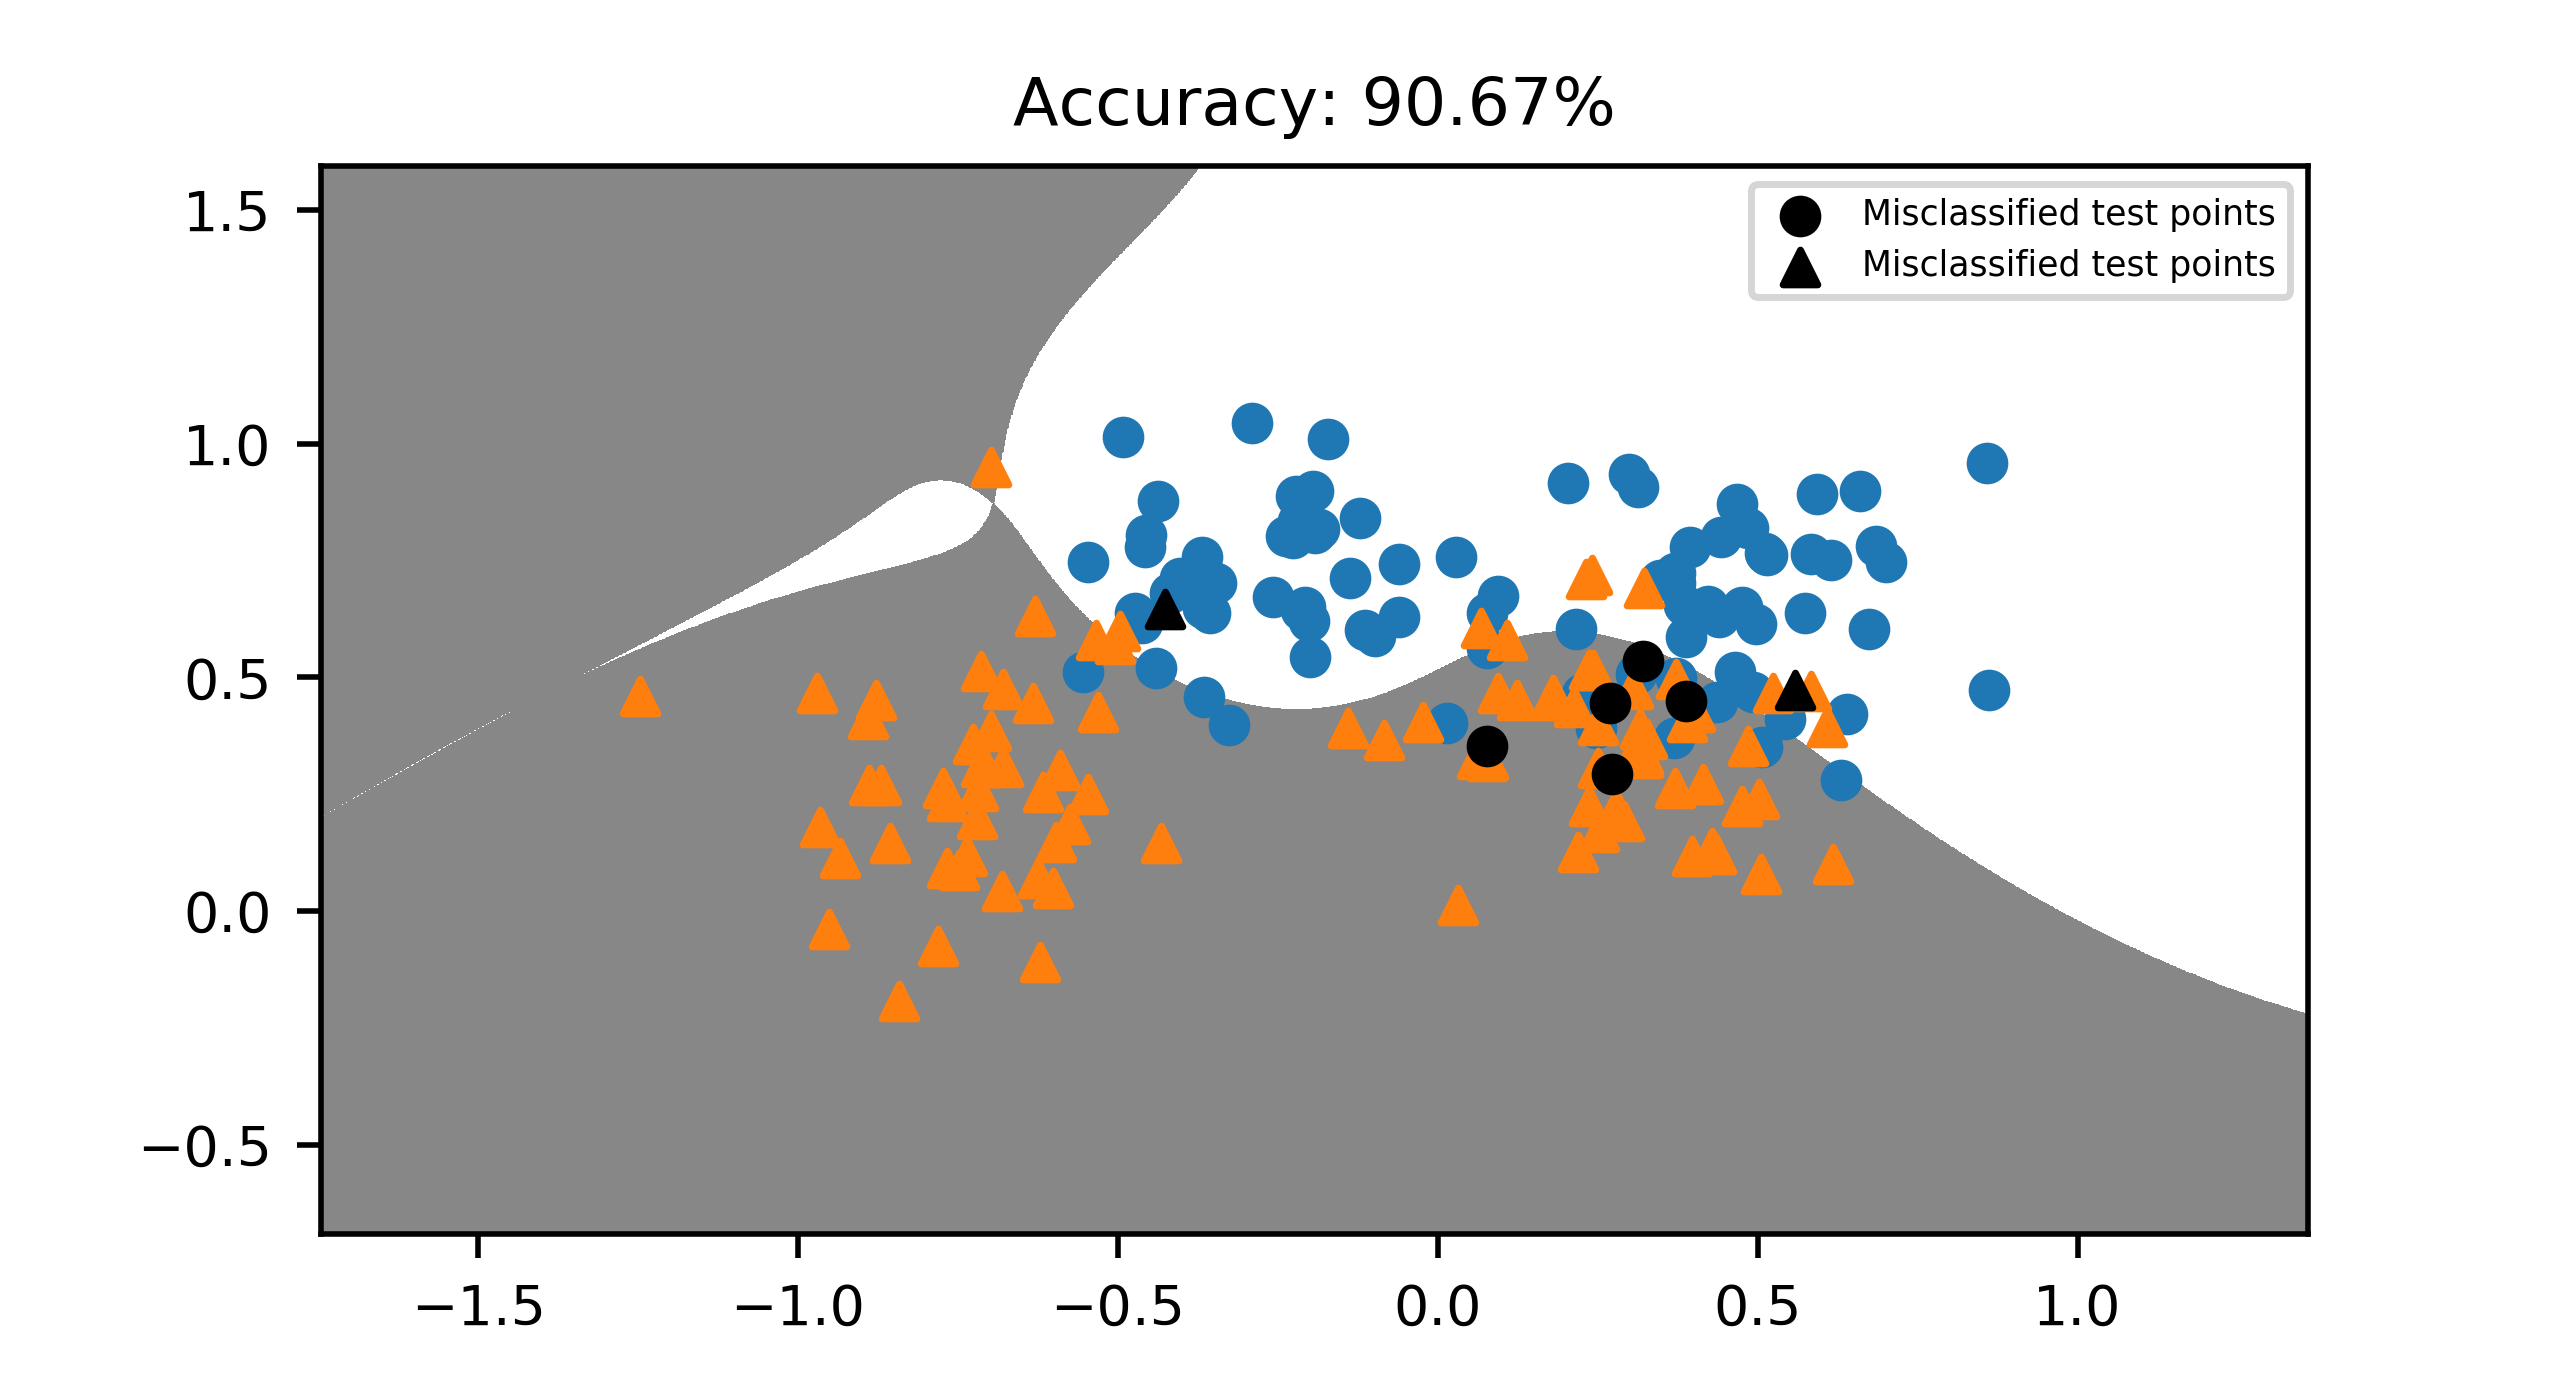
\includegraphics[width=0.5\textwidth]{LSTSVM-Ripley}}
	\subfloat[\lr{KNN-LSTSVM} \lr{($C=2^{-7}, k=6, \gamma=1$)}]{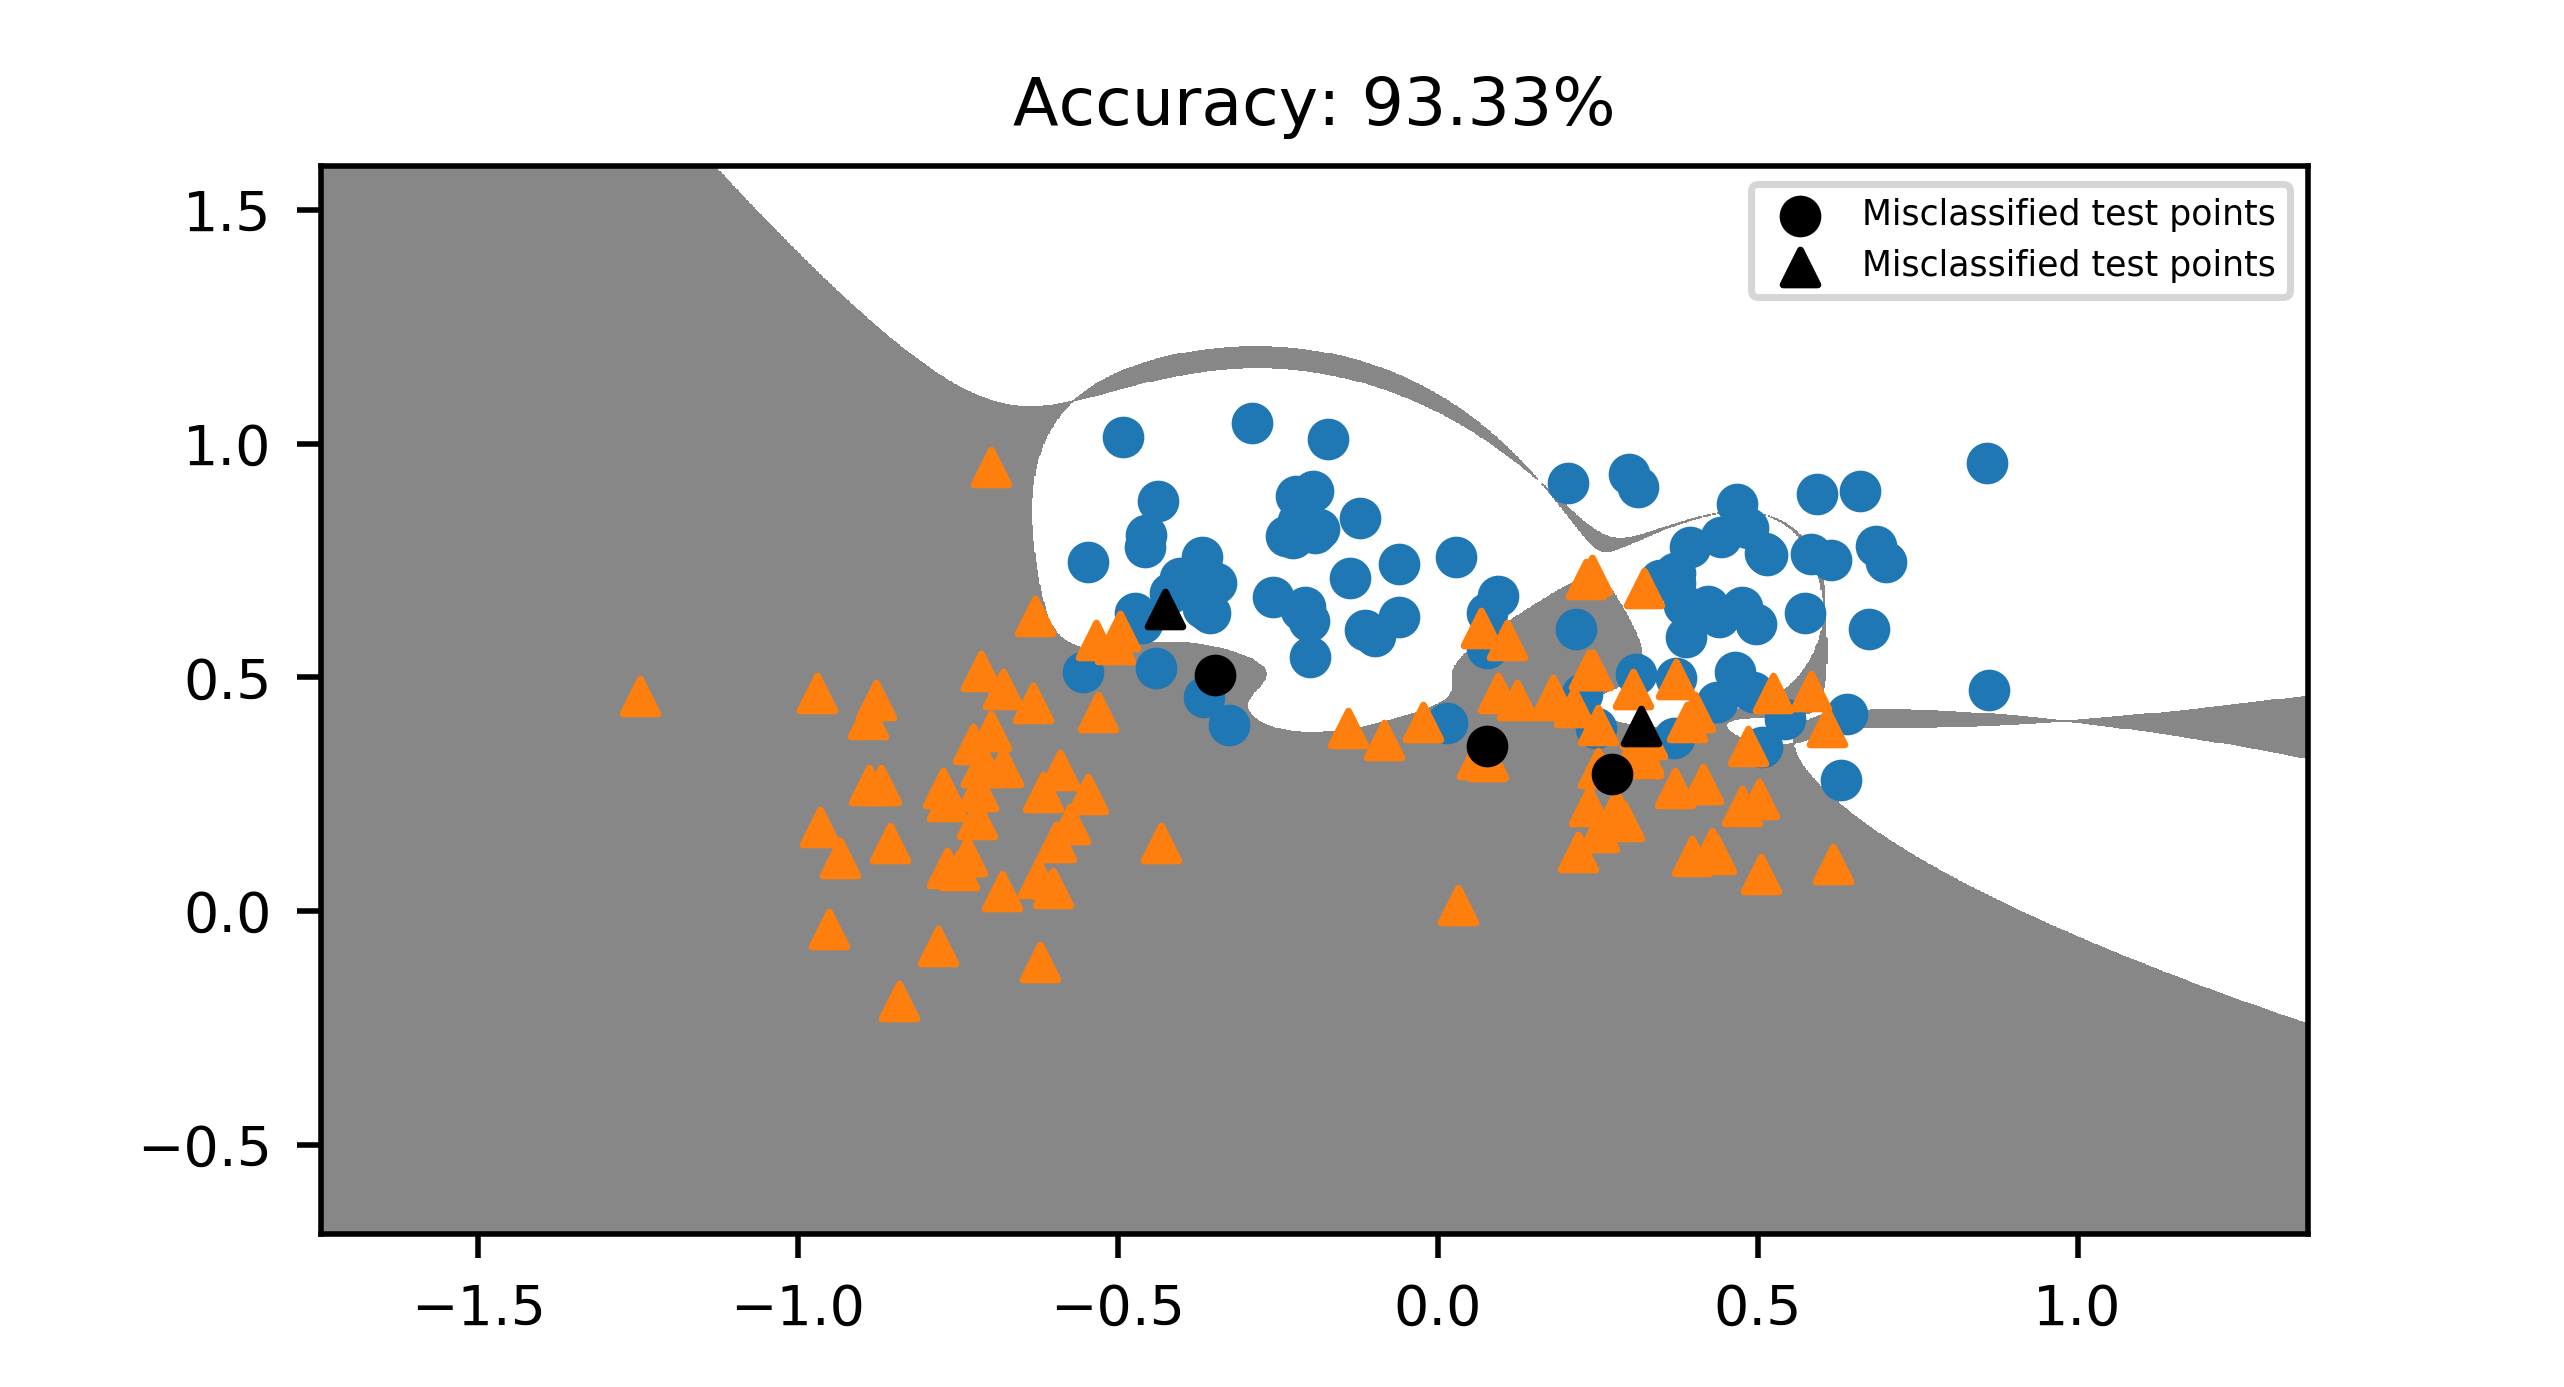
\includegraphics[width=0.5\textwidth]{KNN-LSTSVM-Ripley}}
	\caption{عملکرد و ناحیه تصمیم روش  \lr{LS-TSVM} و  \lr{KNN-LSTSVM} را برای روی داده  \lr{Ripley}}
		\label{fig:LSTSVM-vs-KNN-LSTSVM-R}
\end{figure}

\begin{figure}[!ht]
	\centering
	\subfloat[\lr{LSTSVM} (\lr{$C=2^{-10}, \gamma=2^{1}$})]{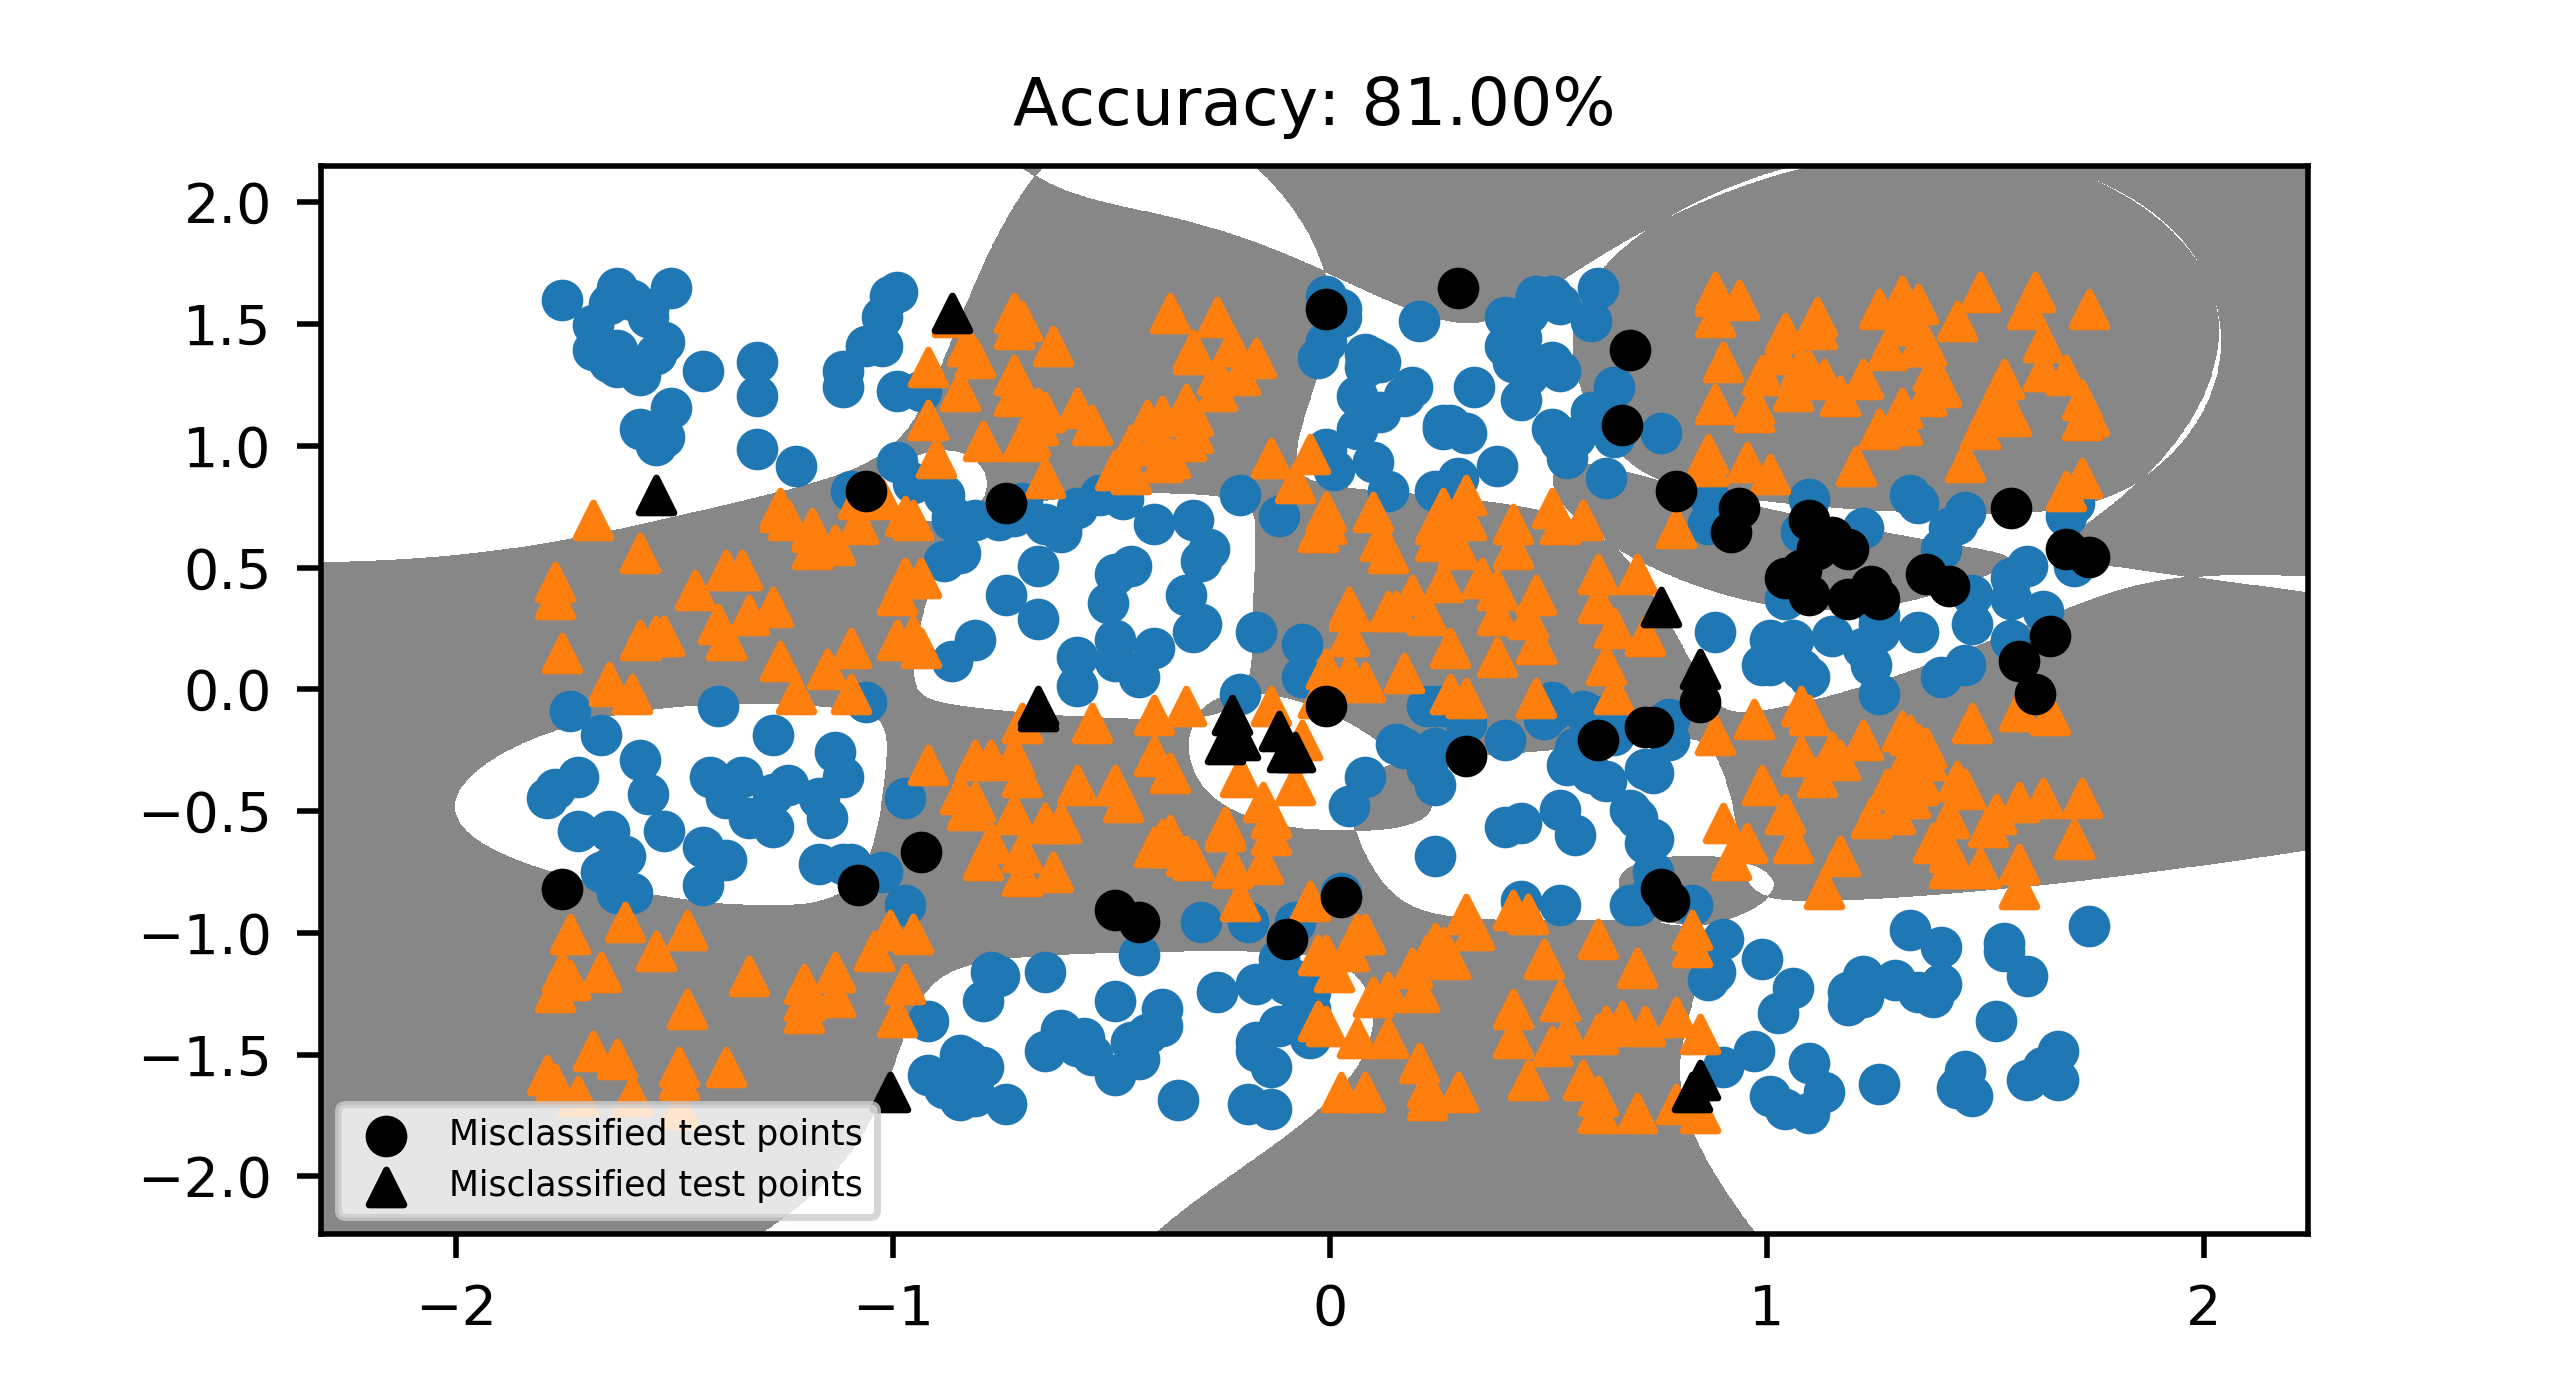
\includegraphics[width=0.5\textwidth]{LSTSVM-check}}
	\subfloat[\lr{KNN-LSTSVM} \lr{($C=2^{-10}, k=6, \gamma=2^{1}$)}]{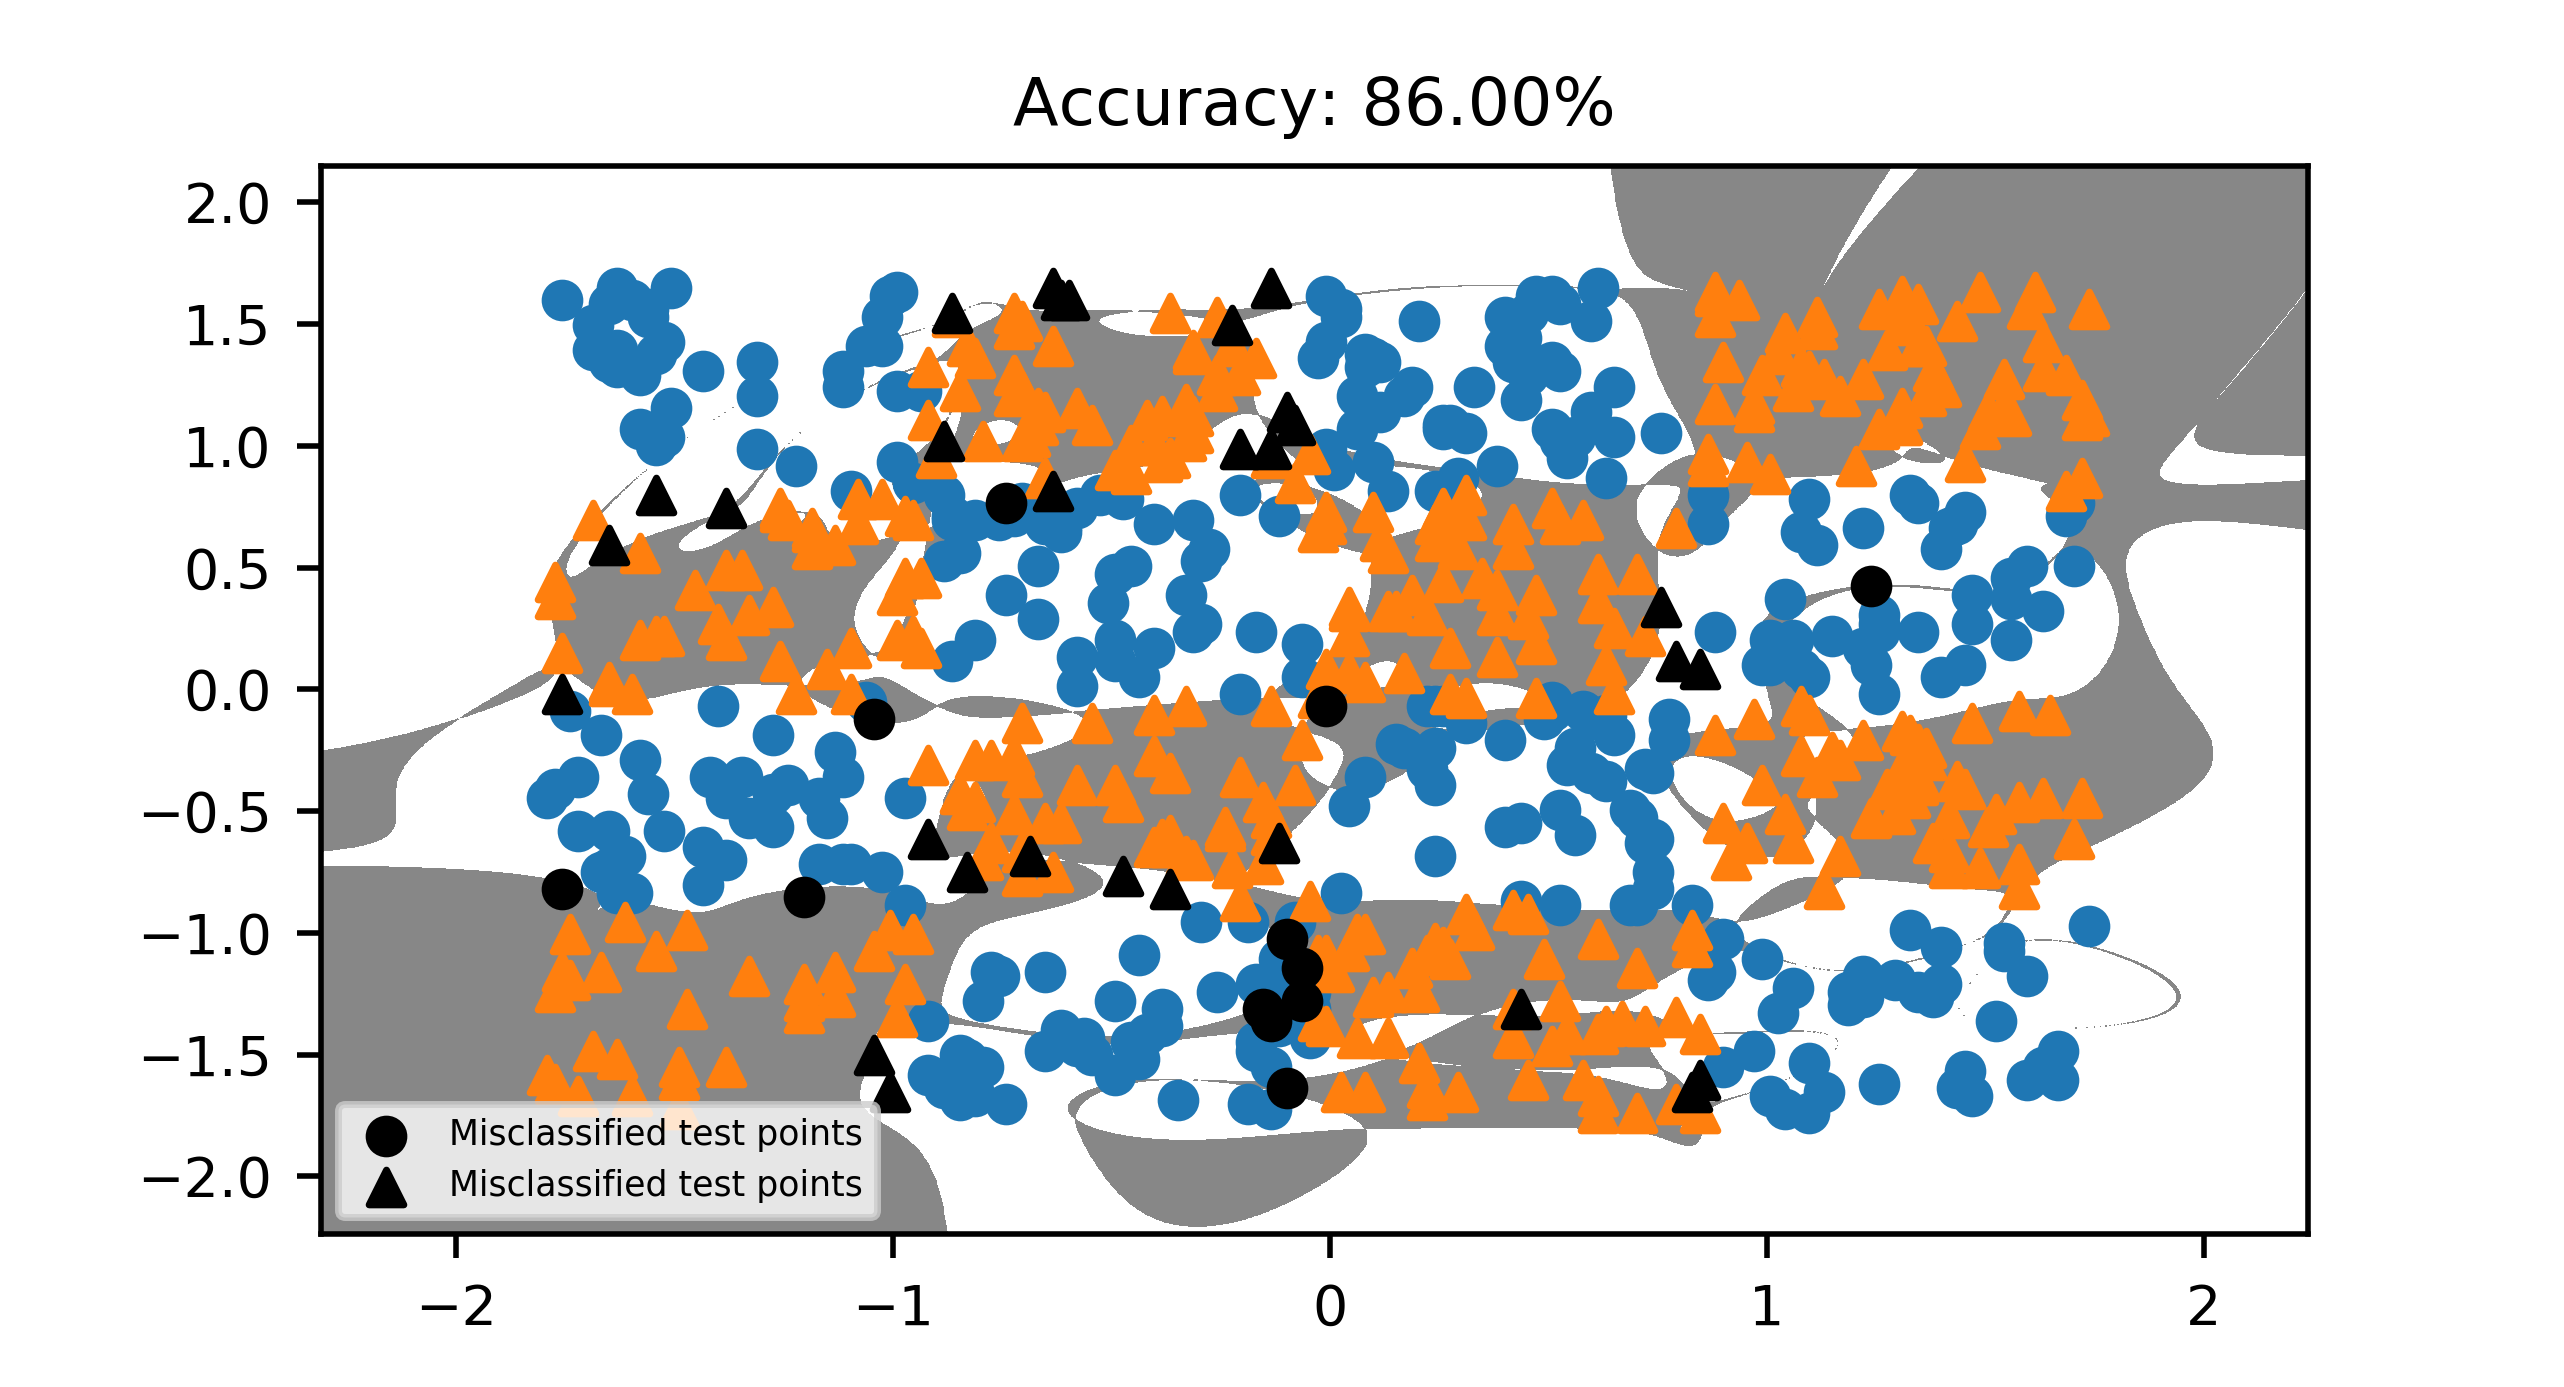
\includegraphics[width=0.5\textwidth]{KNN-LSTSVM-check}}
	\caption{عملکرد و ناحیه تصمیم روش  \lr{LS-TSVM} و  \lr{KNN-LSTSVM} را برای روی داده  \lr{Checkerboard}}
	\label{fig:LSTSVM-vs-KNN-LSTSVM-C}
\end{figure}

\newpage

\subsection{نتایج ارزیابی بر روی مجموعه داده \lr{UCI}}\label{sec:5:2:3}
در این زیر بخش، عملکرد روش \lr{KNN-LSTSVM} روی 14 مجموعه داده از مخرن  \lr{UCI}\LTRfootnote{\lr{https://archive.ics.uci.edu/ml/index.php}} ارزیابی و بررسی می‌شود. مشخصات این مجموعه داده‌ها در جدول \ref{tab:1} ذکر شده است.

\begin{table}[!t]
	\centering
	\caption{مشخصات مجموعه داده‌ها برای ارزیابی روش \lr{KNN-LSTSVM}}
	%\tabcolsep=0.11cm
	\begin{tabular}{l c c c c}
		\hline
		% after \\: \hline or \cline{col1-col2} \cline{col3-col4} ...
		مجموعه داده & تعداد نمونه‌ها & نمونه‌های مثبت & نمونه‌های منفی &تعداد ویژگی‌ها \\
		\hline
	\lr{{Austrailian}} & {690} & {307} & {383} & {14} \\
	\lr{{Bupa-Liver}} & {345} & {145} & {200} & {6} \\
	\lr{{Cleveland}} & {303} & {139} & {164} & {13} \\
	\lr{{Haber-Man}} & {306} & {225} & {81} & {3} \\
	\lr{{Heart-Statlog}} & {270} & {120} & {150} & {13} \\
	\lr{{Hepatits}} & {155} & {32} & {123} & {19} \\
	\lr{{Ionsphere}} & {351} & {225} & {126} & {34} \\
	\lr{{Monk3}} & {554} & {288} & {266} & {6} \\
	\lr{{Pima-Indian}} & {768} & {268} & {500} & {8} \\
	\lr{{Sonar}} & {208} & {97} & {111} & {60} \\
	\lr{{Titanic}} & {891} & {342} & {549} & {7} \\
	\lr{{Votes}} & {435} & {267} & {168} & {16} \\
	\lr{{Wdbc}} & {569} & {212} & {357} & {30} \\
	\lr{{Wpbc}} & {198} & {47} & {151} & {33} \\
		\hline
	\end{tabular}
	
	\label{tab:1}
\end{table}

دقت دسته‌بندی هر کدام از روش‌ها توسط معیار ارزیابی اعتبارسنج ضربدری  ۱۰تایی سنجیده می‌شود. بطوریکه نمونه‌های آموزشی به صورت تصادفی به 10 بخش تقیسم می‌شوند. یکی از این بخش‌ها به عنوان نمونه‌های تست در نظر گرفته می‌شود و سایر بخش‌ها برای آموزش دسته‌بند استفاده می‌گردد. این فرآیند 10 بار تکرار می‌شود تا زمانی که تمام بخش‌ها به عنوان نمونه تست استفاده شود \cite{bishop2006}.

جدول ‏5 2 میانگین و انحراف معیار دقت (به درصد) را برای دسته‌بندهای \lr{TSVM}، \lr{WLTSVM}، \lr{LSTSVM} و \lr{KNN-LSTSVM }نشان می‌دهد. همچنین زمان آموزش دسته‌بندها (به ثانیه) و مقادیر بهینه ‍پارامترها نیز در جدول ‏\ref{tab:3} درج شده است. لازم به ذکر است که محاسبه گراف نزدیک‌ترین همسایه در زمان آموزش دسته‌بندهای \lr{WLTSVM} و \lr{KNN-LSTSVM} لحاظ شده است. 

\begin{table*}[!t]
	\small
	\centering
	\caption{مقایسه دقت و زمان آموزش دسته‌بندهای \lr{TSVM}، \lr{WLTSVM}،  \lr{LSTSVM} و \lr{KNN-LSTSVM}}
	\ra{1.3} % Space between rows
	\tabcolsep=0.13cm % Adjusts column width
	\resizebox{\textwidth}{!}{\begin{tabular}{p{1.95cm} p{1.95cm} p{1.1cm} c p{1.95cm} p{1.1cm} c p{1.95cm} p{1.1cm} c p{1.95cm} p{1.1cm}}
		\toprule
		
		% after \\: \hline or \cline{col1-col2} \cline{col3-col4} ...
		مجموعه داده & \multicolumn{2}{c}{\lr{TSVM}} && \multicolumn{2}{c}{\lr{WLTSVM}} && \multicolumn{2}{c}{\lr{LSTSVM}} && \multicolumn{2}{c}{\lr{KNN-LSTSVM}} \\
		\cmidrule{2-3} \cmidrule{5-6} \cmidrule{8-9} \cmidrule{11-12}
		($m\times n$) & دقت (\%) & زمان اجرا && دقت (\%) & زمان اجرا && دقت (\%) & زمان اجرا &&  دقت (\%) & زمان اجرا \\
		& $(C_1, C_2, \gamma)$  &  && $(C_, \gamma, k)$ &  && $(C_1, C_2, \gamma)$  &  && $(C, \gamma, k)$  &  \\
		\midrule
		\lr{Australian} & \textbf{$87.97\pm2.75$} & $0.070$ && $87.25\pm3.65$ & $0.264$ && $87.68\pm3.79$ & $0.058$ &&  $87.39\pm3.31$ & $0.230$ \\
		($690\times 14$) & ($2^{-4}, 2^{-4}, 2^{-6}$) &  && ($2^{-1}, 2^{-14}, 6$) &  && ($2^{-7}, 2^{-5}, 2^{-6}$) &  && ($2^{3}, 2^{-13}, 7$) &  \\
		\lr{Bupa-Liver} & $73.62\pm4.77$ & $0.082$ && $74.82\pm3.84$ & $0.193$ && $74.51\pm6.89$ & $0.007$ &&  \textbf{$75.96\pm5.40$} & $0.041$ \\
		($345\times 6$) & ($2^{-3}, 2^{-3}, 2^{-6}$) &  && ($2^{2}, 2^{-7}, 4$) &  && ($2^{5}, 2^{4}, 2^{-6}$) &  && ($2^{10}, 2^{-6}, 7$) &  \\
		\lr{Cleveland} & $84.86\pm3.76$ & $0.037$ && $84.48\pm6.29$ & $0.082$ && $85.49\pm4.92$ & $0.005$ &&  \textbf{$85.51\pm6.41$} & $0.026$ \\
		($303\times 13$) & ($2^{0}, 2^{-1}, 2^{-11}$) &  && ($2^{3}, 2^{-9}, 7$) &  && ($2^{2}, 2^{1}, 2^{-11}$) &  && ($2^{-2}, 2^{-15}, 5$) &  \\
		\lr{Haber-Man} & $76.14\pm3.60$ & $0.082$ && $75.80\pm5.22$ & $0.138$ && $76.73\pm7.83$ & $0.005$ &&  \textbf{$76.81\pm5.82$} & $0.031$ \\
		($306\times 3$) & ($2^{1}, 2^{-1}, 2^{-9}$) &  && ($2^{3}, 2^{-4}, 2$) &  && ($2^{9}, 2^{9}, 2^{-7}$) &  && ($2^{-10}, 2^{-9}, 9$) &  \\
		\lr{Heart-Statlog} & \textbf{$85.56\pm5.84$} & $0.041$ && $85.19\pm5.49$ & $0.032$ && $85.19\pm6.20$ & $0.004$ &&  $85.19\pm5.74$ & $0.022$ \\
		($270\times 13$) & ($2^{1}, 2^{0}, 2^{-11}$) &  && ($2^{1}, 2^{-13}, 6$) &  && ($2^{0}, 2^{-1}, 2^{-12}$) &  && ($2^{-1}, 2^{-14}, 7$) &  \\
		\lr{Hepatits} & $85.79\pm8.65$ & $0.003$ && $86.50\pm8.79$ & $0.040$ && \textbf{$87.79\pm6.57$} & $0.001$ &&  $87.13\pm7.59$ & $0.006$ \\
		($155\times 19$) & ($2^{-4}, 2^{-2}, 2^{-8}$) &  && ($2^{8}, 2^{-3}, 3$) &  && ($2^{3}, 2^{5}, 2^{-11}$) &  && ($2^{-1}, 2^{-5}, 7$) &  \\
		\lr{Ionsphere} & \textbf{$92.59\pm3.19$} & $0.028$ && $92.04\pm5.50$ & $0.126$ && $91.74\pm4.32$ & $0.006$ &&  \textbf{$92.59\pm4.47$} & $0.040$ \\
		($351\times 34$) & ($2^{-1}, 2^{-3}, 2^{-5}$) &  && ($2^{1}, 2^{1}, 3$) &  && ($2^{6}, 2^{1}, 2^{-5}$) &  && ($2^{1}, 2^{-5}, 5$) &  \\
		\lr{Monk3} & $98.37\pm1.26$ & $0.150$ && $98.38\pm1.69$ & $0.494$ && $98.55\pm1.36$ & $0.032$ &&  \textbf{$98.56\pm1.34$} & $0.126$ \\
		($554\times 6$) & ($2^{-4}, 2^{2}, 2^{-3}$) &  && ($2^{3}, 2^{-6}, 2$) &  && ($2^{-6}, 2^{-3}, 2^{-3}$) &  && ($2^{0}, 2^{-3}, 5$) &  \\
		\lr{Pima-Indian} & $77.87\pm4.73$ & $0.147$ && $77.86\pm3.49$ & $0.566$ && $77.61\pm5.89$ & $0.073$ &&  \textbf{$78.01\pm3.64$} & $0.339$ \\
		($768\times 8$) & ($2^{1}, 2^{1}, 2^{-3}$) &  && ($2^{4}, 2^{-5}, 2$) &  && ($2^{-1}, 2^{-1}, 2^{-4}$) &  && ($2^{-1}, 2^{-4}, 10$) &  \\
		\lr{Sonar} & $86.14\pm8.35$ & $0.012$ && \textbf{$87.50\pm3.17$} & $0.033$ && $85.55\pm8.31$ & $0.002$ &&  $87.48\pm6.65$ & $0.011$ \\
		($208\times 60$) & ($2^{-5}, 2^{-1}, 2^{-3}$) &  && ($2^{5}, 2^{-4}, 7$) &  && ($2^{-10}, 2^{3}, 2^{-3}$) &  && ($2^{-4}, 2^{-6}, 4$) &  \\
		\lr{Titanic} & $81.94\pm3.23$ & $0.225$ && $81.49\pm4.70$ & $0.692$ && \textbf{$82.38\pm4.63$} & $0.108$ &&  $82.27\pm3.80$ & $0.486$ \\
		($891\times 7$) & ($2^{-4}, 2^{-5}, 2^{-3}$) &  && ($2^{0}, 2^{-6}, 7$) &  && ($2^{1}, 2^{1}, 2^{-5}$) &  && ($2^{8}, 2^{-5}, 10$) &  \\
		\lr{Votes} & $96.78\pm2.11$ & $0.145$ && $97.01\pm1.79$ & $0.098$ && \textbf{$97.02\pm2.89$} & $0.012$ &&  $97.01\pm3.11$ & $0.064$ \\
		($435\times 16$) & ($2^{-6}, 2^{-3}, 2^{-6}$) &  && ($2^{7}, 2^{-13}, 7$) &  && ($2^{-6}, 2^{-3}, 2^{-9}$) &  && ($2^{6}, 2^{-9}, 3$) &  \\
		\lr{Wdbc} & \textbf{$98.42\pm1.23$} & $0.003$ && $97.54\pm2.51$ & $0.206$ && $98.07\pm2.54$ & $0.034$ &&  $97.72\pm1.12$ & $0.154$ \\
		($569\times 30$) & ($2^{-3}, 2^{-1}, 2^{-8}$) &  && ($2^{-2}, 2^{-5}, 6$) &  && ($2^{-4}, 2^{-2}, 2^{-8}$) &  && ($2^{-5}, 2^{-7}, 5$) &  \\
		\lr{Wpbc} & $82.39\pm9.20$ & $0.006$ && $80.84\pm8.94$ & $0.019$ && $81.32\pm9.01$ & $0.002$ &&  \textbf{$82.76\pm5.48$} & $0.010$ \\
		($198\times 33$) & ($2^{-4}, 2^{-5}, 2^{-6}$) &  && ($2^{1}, 2^{-10}, 2$) &  && ($2^{-2}, 2^{-4}, 2^{-7}$) &  && ($2^{-2}, 2^{-7}, 6$) &  \\
		\midrule
		میانگین دقت  & \multicolumn{2}{c}{$86.31$} && \multicolumn{2}{c}{$86.19$} && \multicolumn{2}{c}{$86.40$} && \multicolumn{2}{c}{\textbf{$86.74$}} \\
		\bottomrule
	\end{tabular}}
	
	\label{tab:3}
\end{table*}

نتایج بدست آمده به این صورت تحلیل و بررسی می‌شود:
\begin{enumerate}
	\item از نظر دقت دسته‌بندی، روش پیشنهادی (\lr{KNN-LSTSVM}) از سه روش دیگر بهتر عمل کرده است. زیرا روش \lr{KNN-LSTSVM} با استفاده از گراف نزدیک‌ترین همسایه، اطلاعات شباهت نمونه‌ها را در تابع هدف لحاظ می‌کند. از این رو ابرصفحه غیر موازی در روش پیشنهادی به نمونه‌های پرتراکم نزدیک‌تر و از نمونه‌های حاشیه‌ای حداکثر فاصله را می‌گیرد. در حالی که روش‌های \lr{TSVM} و \lr{LSTSVM}  نمونه‌های حاشیه‌ای را در نظر نمی‌گیرد.
	\item از نظر زمان آموزش و پیچیدگی محاسباتی، روش \lr{LSTSVM} از سایر روشها سریع‌تر است. زیرا در این روش فقط دو دستگاه معادلات خطی حل می‌گردد. با این حال روش پیشنهادی (\lr{KNN-LSTSVM}) از روش \lr{WLTSVM} و \lr{TSVM} به طور قابل توجه‌ای سریع‌تر است. زیرا روش پیشنهادی دو دستگاه معادلات خطی حل می‌کند، در حالی‌که روش \lr{WLTSVM} و \lr{TSVM} دو مسئله دوگان درجه دو را حل می‌کنند.
	\item به منظور بررسی اثر پارامتر  $k$ روی دقت روش \lr{KNN-LSTSVM}، آزمایش روی مجموعه داده‌های \lr{Australian} و \lr{Hepatitis} صورت گرفته است. مقادیر پارامتر  $k$ بین 2 تا 30 با گام 2 تعیین شده است. شکل ‏ \ref{fig:KNN-LSTSVM-Aust-Hepa} اهمیت انتخاب پارامتر   را نشان می‌دهد. بیشترین دقت برای مجموعه داده \lr{Australian} با پارامتر  $k=12$ بدست آمده است. به عبارت دیگر،  پارامتر بهینه برای مجموعه داده \lr{Australian} می‌باشد. از طرف دیگر، افزایش مقدار  $k$ برای مجموعه داده \lr{Hepatitis} باعث بهبود دقت روش \lr{KNN-LSTSVM} می‌شود. به طور کلی، انتخاب بهینه پارامتر  $k$ روی عملکرد روش پیشنهادی تاثیر زیادی دارد.
\end{enumerate}

\begin{figure}[!t]
	\centering
	\subfloat[مجموعه داده \lr{Australian}]{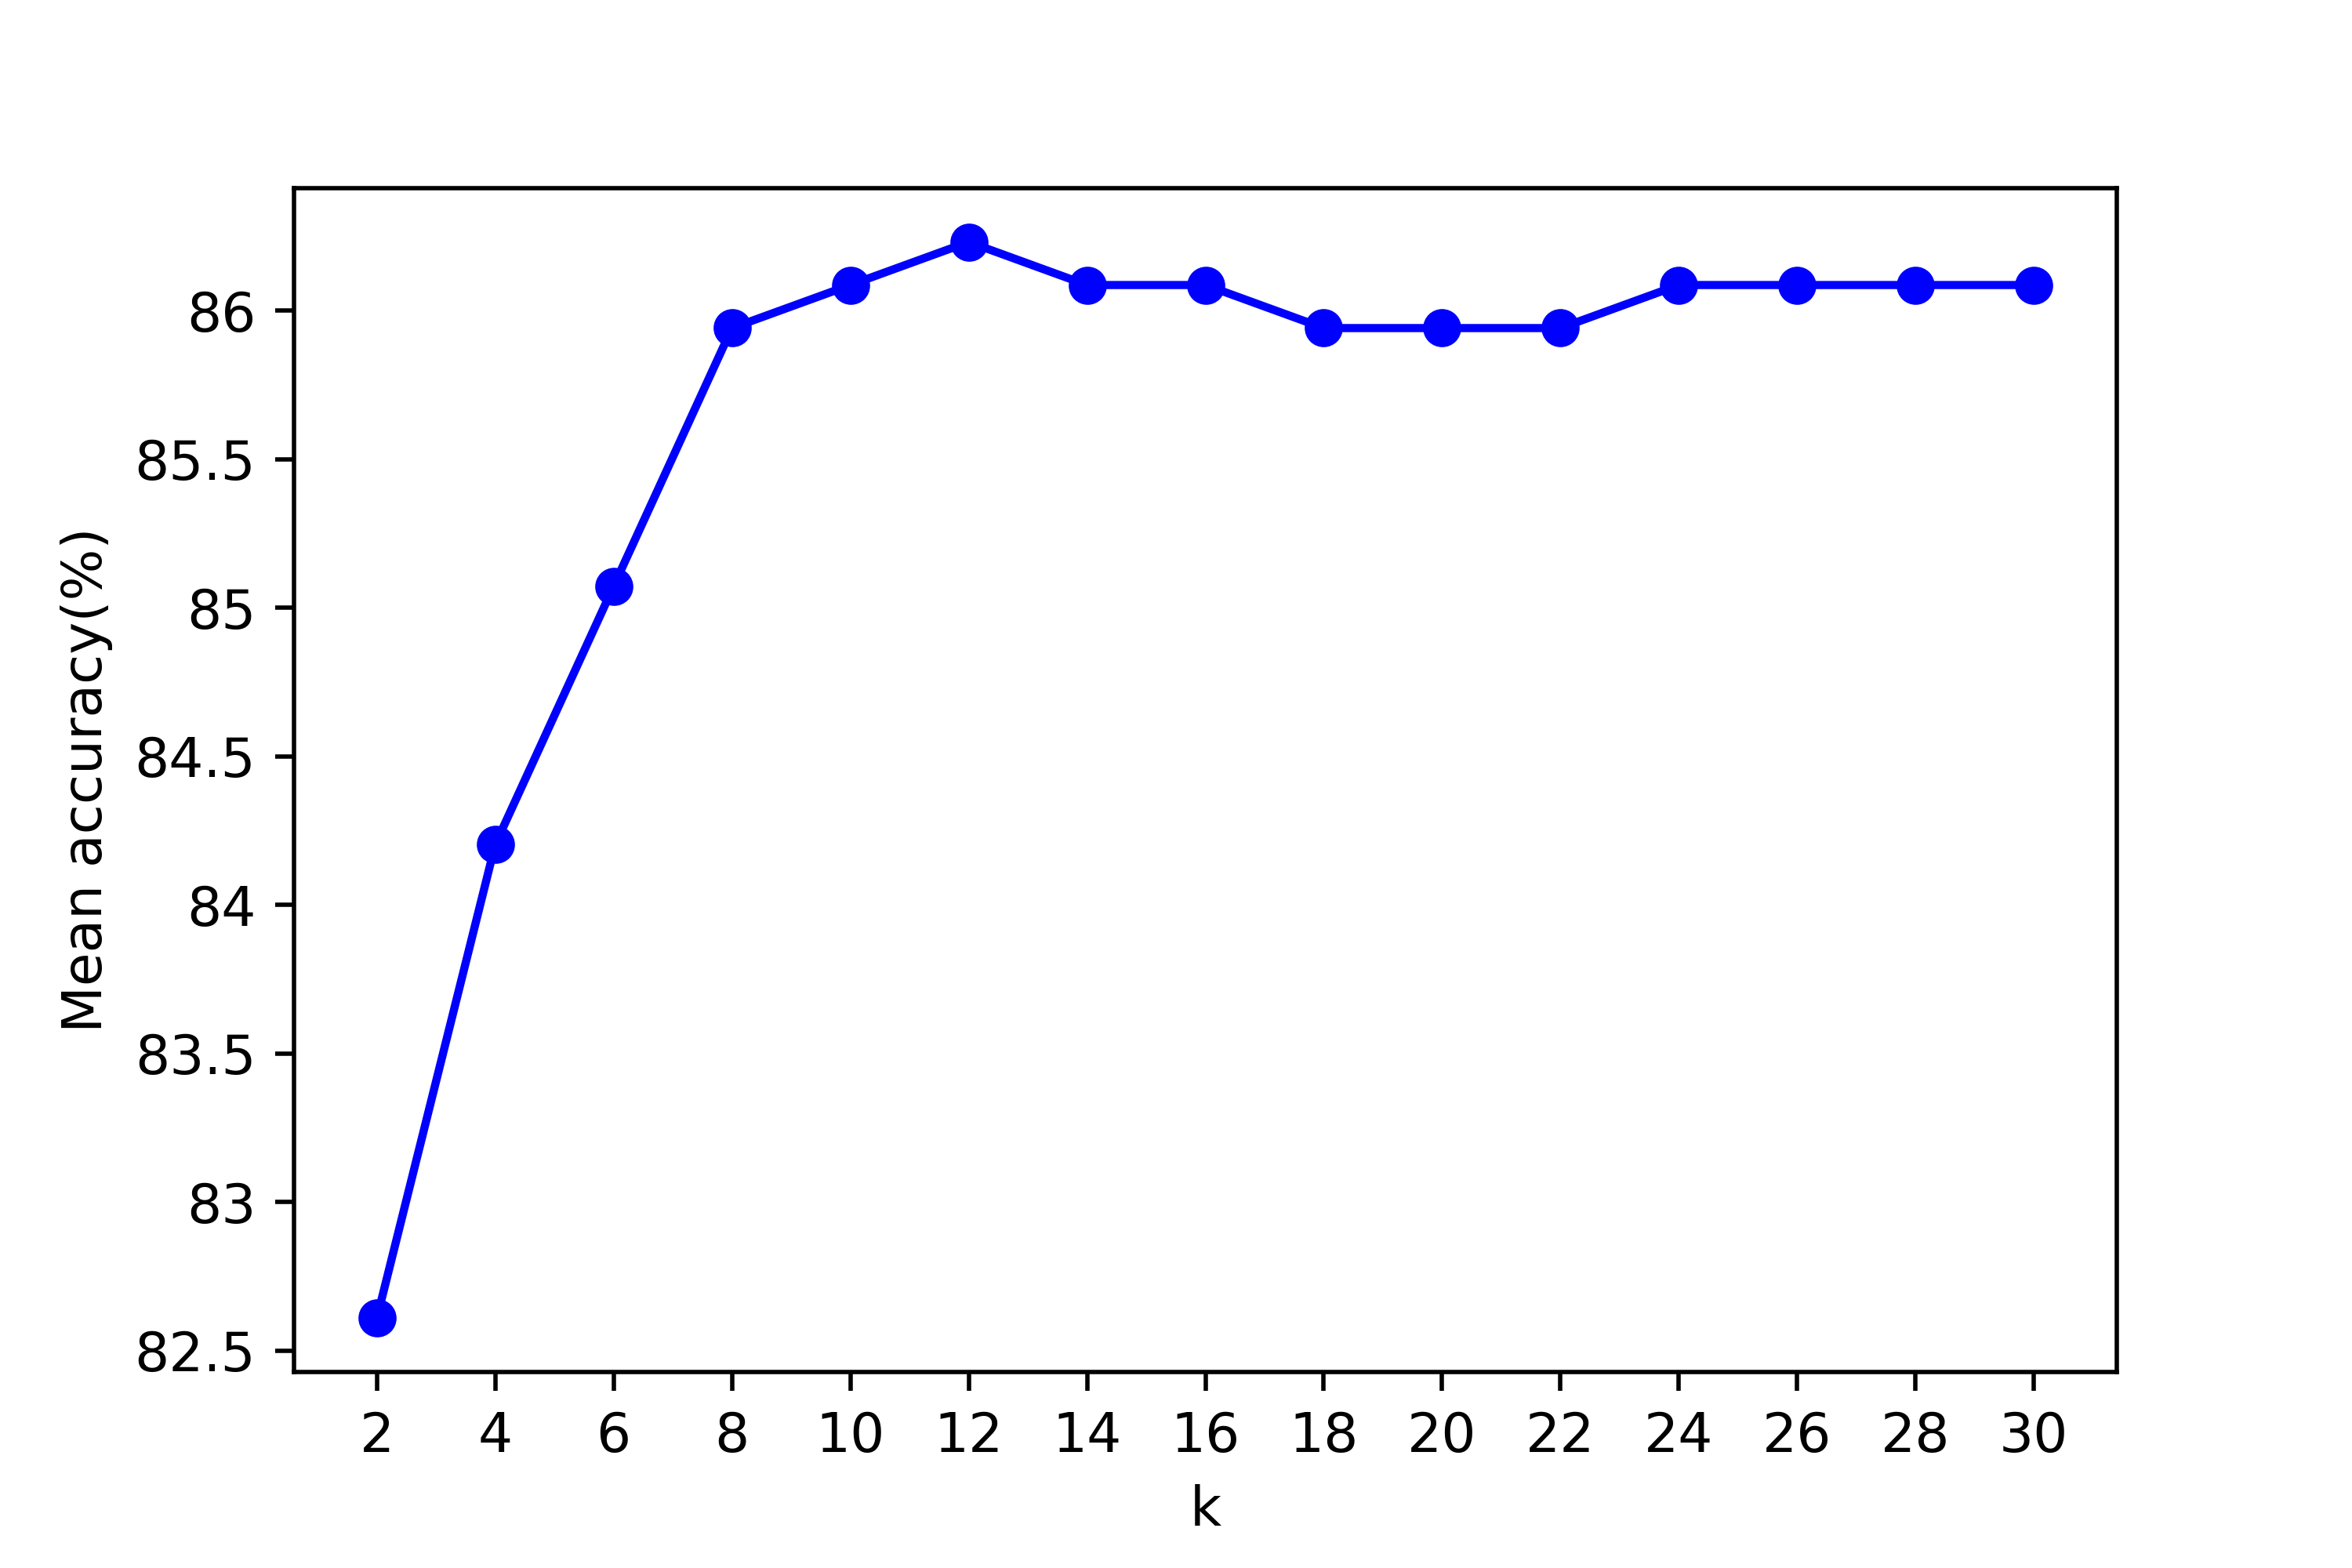
\includegraphics[width=0.5\textwidth]{KNN-LSTSVM-Aust}}
	\subfloat[مجموعه داده \lr{Hepatitis}]{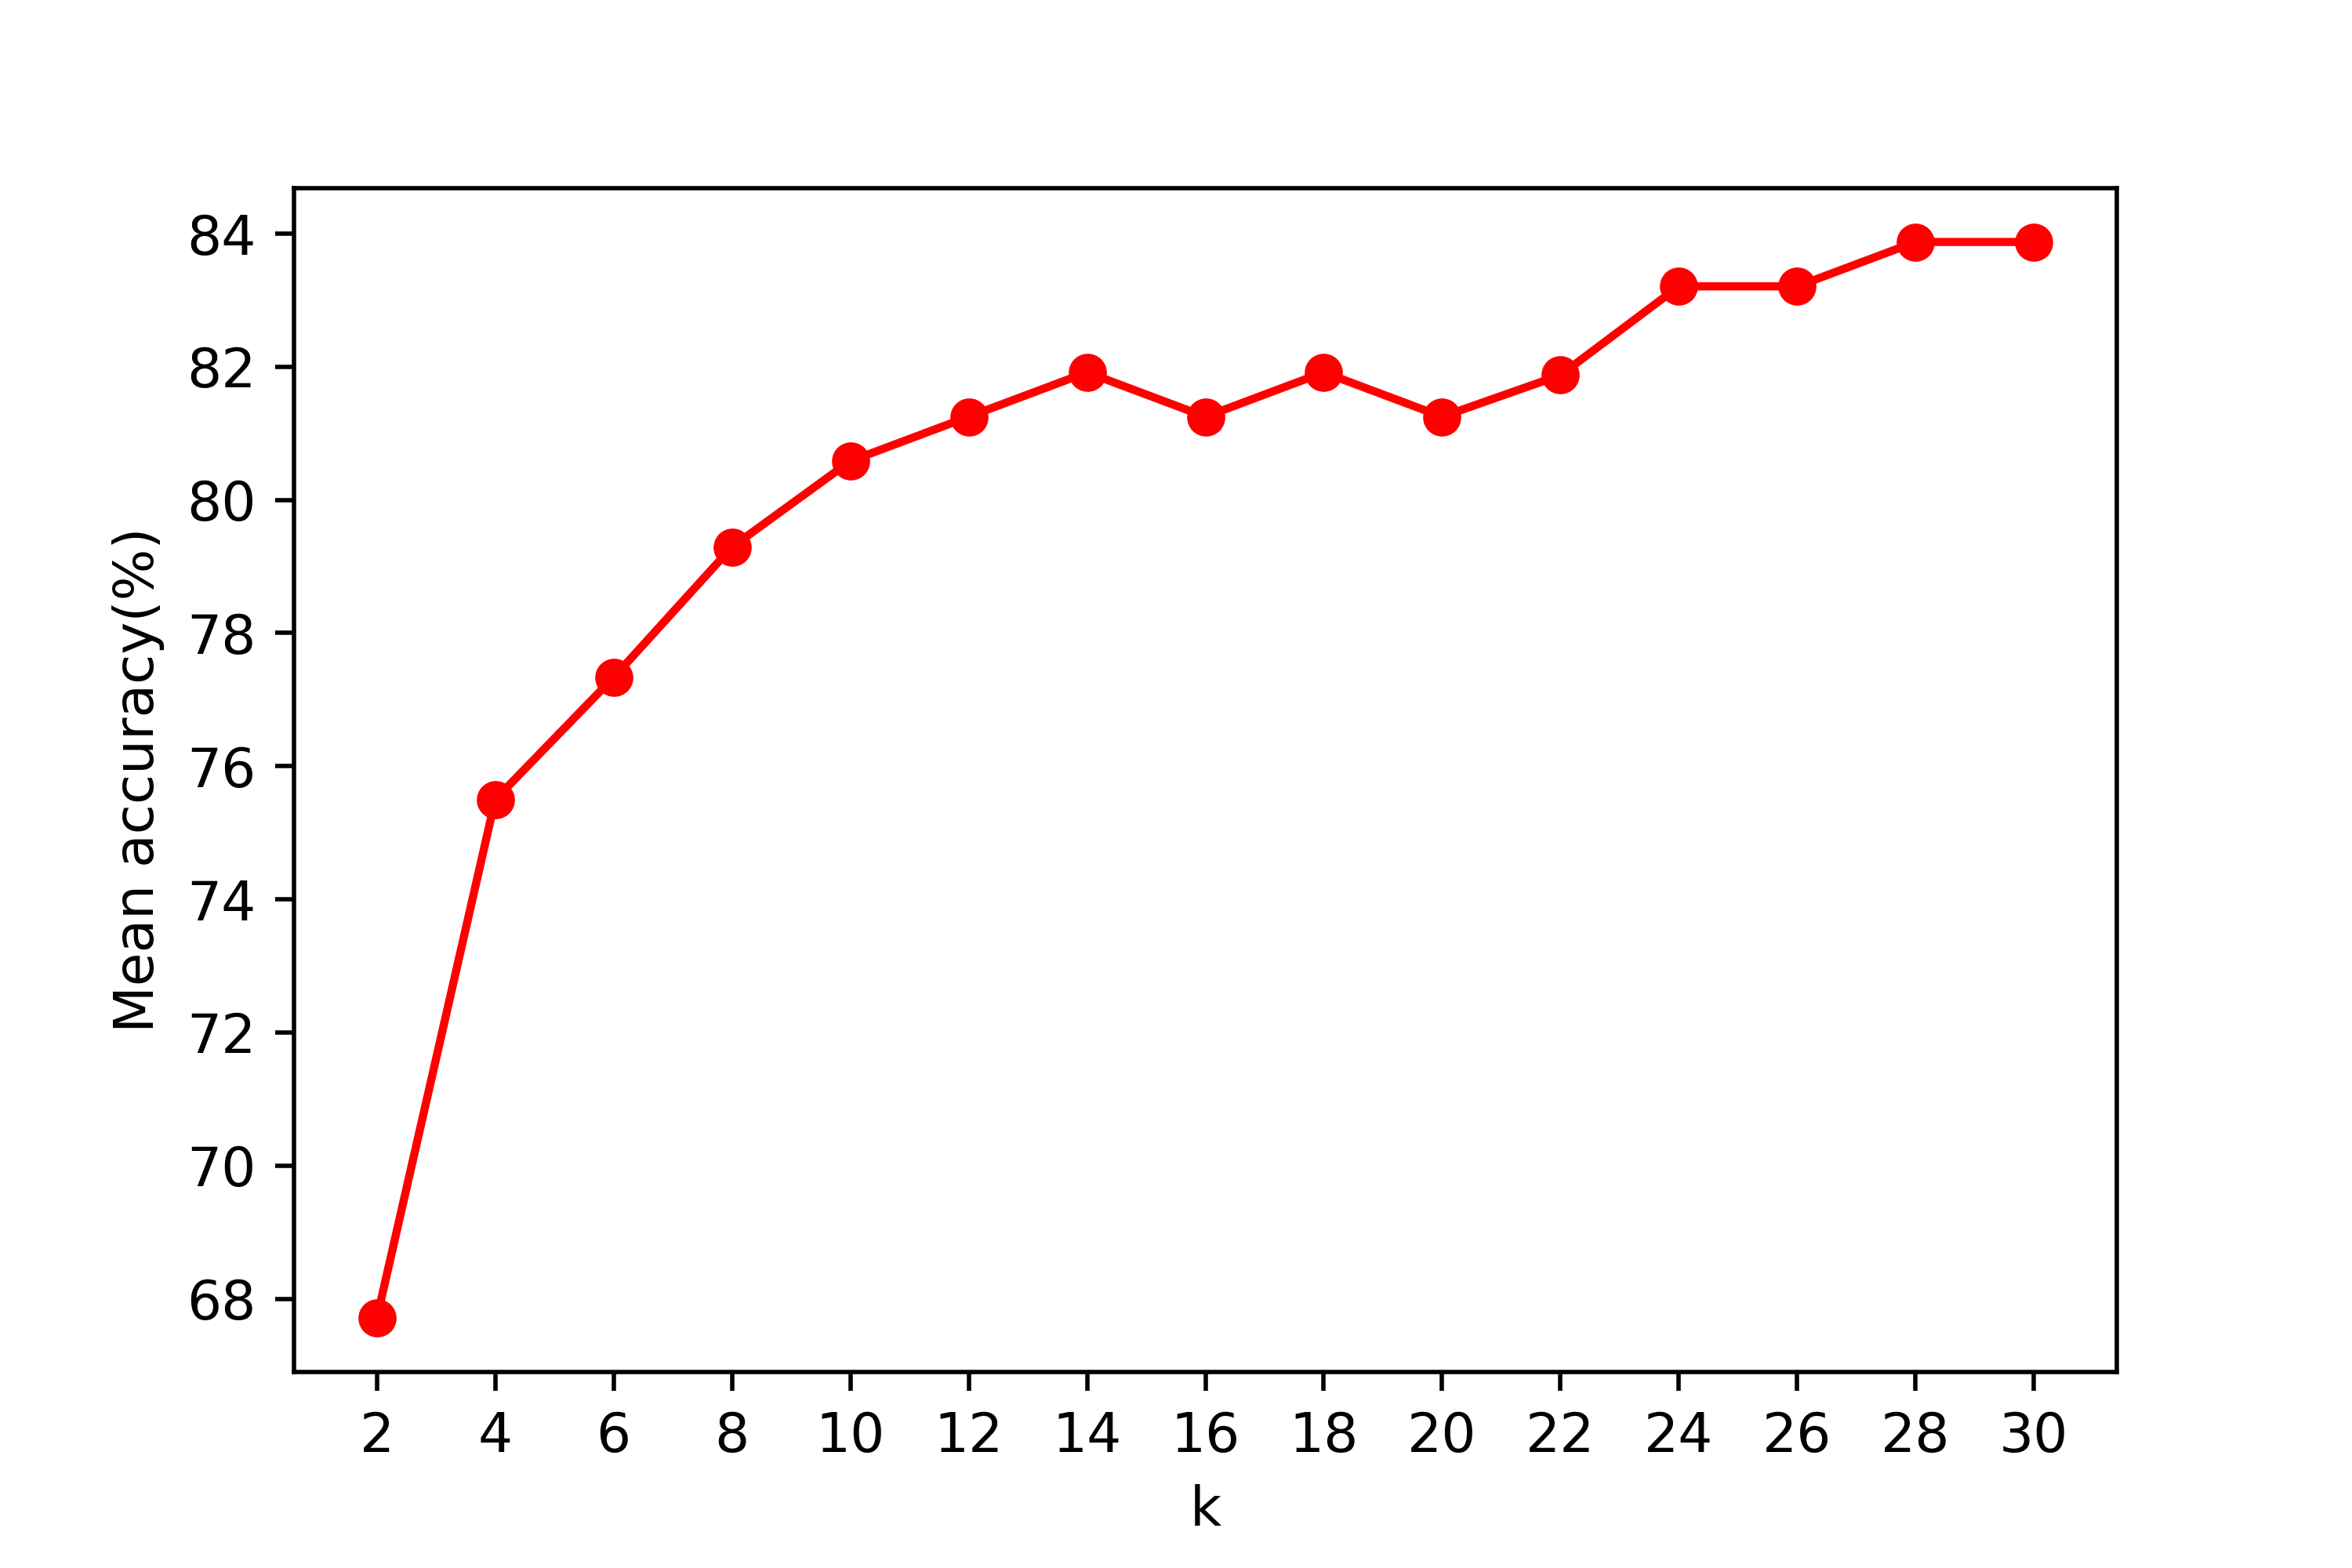
\includegraphics[width=0.5\textwidth]{KNN-LSTSVM-Hepa}}
	\caption{اثر افزایش پارامتر $k$ روی دقت دسته‌بند \lr{KNN-LSTSVM}}
	\label{fig:KNN-LSTSVM-Aust-Hepa}
\end{figure}

\subsubsection{بررسی آماری}\label{sec:5:2:3:1}
به منظور تحلیل بیشتر عملکرد چهار روش روی 14 مجموعه داده (\ref{tab:3})، آزمون‌های آماری طبق پیشنهاد دمسار\LTRfootnote{\lr{Demsar}} \cite{demsar2006} استفاده می‌شود. بدین منظور آزمون آماری ساده و ناپارامتریک فریدمن\LTRfootnote{\lr{Friedman}}  مورد استفاده قرار گرفته است. به منظور انجام آزمون آماری، میانگین رتبه چهار روش بر اساس دقت محاسبه شده و در جدول ‏\ref{tab:4} نشان داده شده است. ابتدا بر اساس فرض صفر، تمام روش‌ها را یکسان در نظر می‌گیریم. سپس آزمون فریدمن با رابطه زیر محاسبه می‌شود.
\begin{equation}\label{eq:5:1}
\chi^2_F = \frac{12N}{k(k + 1)}\bigg[\sum_{j} R^2_j - \frac{k(k + 1)^2}{4} \bigg],
\end{equation}

در رابطه \ref{eq:5:1}،  $R_j=\frac{1}{N}\sum_{i}r^j_i$ و $r_{i}^{j}$  نشان‌دهنده رتبه $j$مین روش بر روی $i$مین مجموعه داده از  $N$ است. 

\begin{table}[!t]
	\centering
	\caption{میانگین رتبه براساس دقت (ارزیابی \lr{KNN-LSTSVM})}
	\ra{1.3} % Space between rows
	\tabcolsep=0.10cm
	\begin{tabular}{c c c c c c c c c c c c}
		\toprule
		% after \\: \hline or \cline{col1-col2} \cline{col3-col4} ...
		مجموعه داده & \lr{TSVM} & \lr{WLTSVM} & \lr{LSTSVM} & \lr{KNN-LSTSVM} \\
		\midrule
	\lr{Austrailian} & 1 & 4 & 2 & 3\\
	\lr{Bupa-Liver} & 4 & 2 & 3 & 1\\
	\lr{Cleveland} & 3 & 4 & 2 & 1\\
	\lr{Haber-Man} & 3 & 4 & 2 & 1\\
	\lr{Heart-Statlog} & 1 & 3 & 3 & 3\\
	\lr{Hepatits} & 4 & 3 & 1 & 2\\
	\lr{Ionsphere} & $1.5$ & 3 & 4 & $1.5$\\
	\lr{Monk3} & 4 & 3 & 2 & 1\\
	\lr{Pima-Indian} & 2 & 3 & 4 & 1\\
	\lr{Sonar} & 3 & 1 & 4 & 2\\
	\lr{Titanic} & 3 & 4 & 1 & 2\\
	\lr{Votes} & 4 & $2.5$ & 1 & $2.5$\\
	\lr{Wdbc} & 1 & 4 & 2 & 3\\
	\lr{Wpbc} & 2 & 4 & 3 & 1\\
	میانگین رتبه & $2.61$ & $3.18$ & $2.43$ & \textbf{$1.79$} \\
		\bottomrule
	\end{tabular}
	
	\label{tab:4}
\end{table}

سپس مقدار $F_F$  براساس  $\chi^2_F$ به صورت زیر محاسبه می‌شود. بطوریکه $F_F$ از توزیع $F$ با $(k-1)$ و $(k-1)(N-1)$ درجه آزادی پیروی می‌کند.
\begin{equation}\label{eq:5:2}
F_F = \frac{(N - 1)\chi^2_F}{N(k - 1) - \chi^2_F}
\end{equation}

بر اساس روابط \ref{eq:5:1} و \ref{eq:5:2}، مقادیر $\chi^2_F = 8.293$ و  $F_F = 3.198$ بدست آمده است. در اینجا $F_F$ از توزیع $F$  با (39، 3) درجه آزادی پیروی می‌کند. مقادیر ویژه $F(3, 39)$ برای سطوح معناداری 25/0، 1/0 و 05/0 به ترتیب برابر  42/1، 23/2 و 84/2 است. مقدار  $F_F$ به طور قابل توجه‌ای بیشتر از مقدار ویژه است. بنابراین از آزمون آماری استنتاج می‌شود که تفاوت قابل توجه‌ای بین 4 روش وجود دارد. همچنین جدول ‏\ref{tab:6} نشان می‌دهد که روش پیشنهادی (\lr{KNN-LSTSVM}) در مجموع عملکرد بهتری نسبت به سایر روش‌ها دارد. زیرا میانگین رتبه روش پیشنهادی در میان سایر روش‌ها کمترین است.

\subsection{مجموعه داده \lr{NDC}}\label{sec:5:2:4}
به منظور بررسی سرعت آموزش روش پیشنهادی (\lr{RKNN-TSVM}) و مقایسه آن با سایر روش‌ها، آزمایش بر روی مجموعه داده‌های بزرگ صورت گرفته است. مجموعه داده \lr{NDC} \cite{musicant1998} برای این منظور انتخاب شده است. جدول ‏\ref{tab:5} مشخصات این مجموعه داده را نشان می‌دهد.

\begin{table}[!t]
	\centering
	\caption{مشخصات مجموعه داده \lr{NDC}}
	\begin{tabular}{l c c c}
		\toprule
		% after \\: \hline or \cline{col1-col2} \cline{col3-col4} ...
		مجموعه داده & تعداد نمونه‌های آموزش & تعداد نمونه‌های تست & تعداد ویژگی‌ها\\
		\midrule
\lr{{NDC-500}} & {500} & {50} & {32} \\
\lr{{NDC-700}} & {700} & {70} & {32} \\
\lr{{NDC-900}} & {900} & {90} & {32} \\
\lr{{NDC-1K}} & {1000} & {100} & {32} \\
\lr{{NDC-2K}} & {2000} & {200} & {32} \\
\lr{{NDC-3K}} & {3000} & {300} & {32} \\
\lr{{NDC-4K}} & {4000} & {400} & {32} \\
\lr{{NDC-5K}} & {5000} & {500} & {32} \\
\lr{{NDC-10K}} & {10000} & {1000} & {32} \\
\lr{{NDC-25K}} & {25000} & {2500} & {32} \\
\lr{{NDC-50K}} & {50000} & {5000} & {32} \\
		\bottomrule
	\end{tabular}
	
	\label{tab:5}
\end{table}

جهت آزمایش با مجموعه داده \lr{NDC}، پارامتر $C$ برای تمام روش برابر با یک است. در نسخه غیر خطی از تابع \lr{RBF} با پارامتر $\gamma=2^{-15}$ استفاده شده است. همچنین پارامتر  $k$ برای روش‌های \lr{WLTSVM} و \lr{KNN-LSTSVM} برابر با 5 است. جدول \ref{tab:6} زمان آموزش چهار روش بر روی مجموعه داده \lr{NDC} با تابع هسته خطی و \lr{RBF} را نشان می‌دهد.

\begin{sidewaystable*}
%\begin{table*}[!t]
	\centering
	\caption{مقایسه زمان آموزش روش \lr{KNN-LSTSVM} و سایر روش‌ها بر روی مجموعه داده \lr{NDC}}
	\ra{1.3} % Space between rows
	\begin{threeparttable}
		\begin{tabular}{c c c c c c c c c c c c c}
			\toprule
			% after \\: \hline or \cline{col1-col2} \cline{col3-col4} ...
			&& \multicolumn{2}{c}{\lr{TSVM}} && \multicolumn{2}{c}{\lr{WLTSVM}} && \multicolumn{2}{c}{\lr{LSTSVM}} && \multicolumn{2}{c}{\lr{KNN-LSTSVM}} \\
			مجموعه داده && \multicolumn{2}{c}{زمان اجرا} && \multicolumn{2}{c}{زمان اجرا} && \multicolumn{2}{c}{زمان اجرا} && \multicolumn{2}{c}{زمان اجرا} \\
			\cmidrule{3-4} \cmidrule{6-7} \cmidrule{9-10} \cmidrule{12-13}
		&تابع هسته	& خطی & \lr{RBF} && خطی & \lr{RBF} && خطی & \lr{RBF} && خطی & \lr{RBF} \\
			\midrule
			\lr{NDC-500} && $0.222$ & $0.324$ && $0.583$ & $0.838$ && $0.004$ & $0.034$ && $0.031$ & $0.399$ \\
			\lr{NDC-700} && $0.45$ & $0.744$ && $1.115$ & $1.741$ && $0.004$ & $0.064$ && $0.053$ & $0.757$ \\
			\lr{NDC-900} && $0.83$ & $1.111$ && $1.884$ & $2.761$ && $0.004$ & $0.223$ && $0.084$ & $1.362$ \\
			\lr{NDC-1K} && $0.976$ & $1.599$ && $2.315$ & $3.499$ && $0.004$ & $0.266$ && $0.1$ & $1.657$ \\
			\lr{NDC-2K} && $6.606$ & $12.746$ && $16.297$ & $22.474$ && $0.004$ & $1.055$ && $0.387$ & $6.21$ \\
			\lr{NDC-3K} && $25.387$ & $41.908$ && $73.451$ & $70.213$ && $0.004$ & $2.588$ && $0.904$ & $14.041$ \\
			\lr{NDC-4K} && $72.19$ & $129.932$ && $163.249$ & $176.899$ && $0.005$ & $5.314$ && $1.647$ & $25.812$ \\
			\lr{NDC-5K}\lr{\textsuperscript{b}} && $137.909$ & $277.463$ && $319.574$ & $339.347$ && $0.005$ & $10.024$ && $2.618$ & $39.788$ \\
			\lr{NDC-10K}\lr{\textsuperscript{b}} && $696.562$ & \lr{\tnote{a}} && \lr{\tnote{a}} & \lr{\tnote{a}} && $0.007$ & $67.475$ && $11.249$ & $164.655$ \\
			\lr{NDC-25K}\lr{\textsuperscript{b}} && \lr{\tnote{a}} & \lr{\tnote{a}} && \lr{\tnote{a}} & \lr{\tnote{a}} && $0.011$ & $967.458$ && $75.707$ & \lr{\tnote{a}} \\
			\lr{NDC-50K}\lr{\textsuperscript{b}} && \lr{\tnote{a}} & \lr{\tnote{a}} && \lr{\tnote{a}} & \lr{\tnote{a}} && $0.02$ & \lr{\tnote{a}} && $383.829$ & \lr{\tnote{a}} \\
			
			\bottomrule
		\end{tabular}
		\begin{tablenotes}
			\item[\lr{a}] اجرای روش به دلیل زیاد بودن زمان آزمایش خاتمه یافته است.
			\item[\lr{b}] از تابع هسته مستطیلی با اندازه 10 درصد نمونه‌های آموزشی استفاده شده است.
		\end{tablenotes}
	\end{threeparttable}
	\label{tab:6}
%\end{table*}
\end{sidewaystable*}

روش پیشنهادی (\lr{KNN-LSTSVM}) چندین برابر سریع‌تر از روش \lr{WLTSVM} روی تمام مجموعه داده‌های \lr{NDC} ظاهر شده است. زیرا روش پیشنهادی نیازی به الگوریتم‌های حل مسائل بهینه‌سازی ندارد، در حالی‌که روش \lr{WLTSVM} با استفاده از الگوریتم \lr{clipDCD} پیاده‌سازی شده است. همانطور که در جدول \ref{tab:6} مشخص است، روش \lr{KNN-LSTSVM} سریع‌تر از روش \lr{LSTSVM} نمی‌باشد. چون در روش پیشنهادی علاوه بر حل کردن دو دستگاه معادلات خطی، گراف نزدیک‌ترین همسایه نیز برای تمام نمونه‌ها محاسبه می‌شود. 

رویکرد تابع هسته مستطیلی با 10 درصد از نمونه‌ها در نسخه غیر خطی استفاده شده است. نتایج نسخه غیر خطی نشان می‌دهد که روش \lr{KNN-LSTSVM} و \lr{LSTSVM} از روش \lr{WLTSVM} و \lr{TSVM} بسیار سریع‌تر هستند. زیرا حتی با تابع هسته تقلیل یافته  $(m \times \bar{m})$، در روش \lr{WLTSVM} و \lr{TSVM} دو مسئله دوگان حل می‌شود.

به منظور نشان دادن تاثیر پارامتر $k$  بر روی زمان آموزش روش \lr{KNN-LSTSVM}، یک آزمایش بر روی مجموعه داده بزرگ \lr{NDC-10K} انجام گرفته است. همانطور که در شکل \ref{fig:KNN-LSTSVM-k} نشان داده شده است، افزایش پارامتر  $k$ روی زمان آموزش روش پیشنهادی تاثیر بسیار اندکی دارد. به طور خلاصه، نتایج روی مجموعه داده \lr{NDC} نشان می‌دهد که روش \lr{KNN-LSTSVM} نسبت به \lr{TSVM} و \lr{WLTSVM} برای مجموعه داده‌های بزرگ مناسب‌تر است. 

\begin{figure}[!t]
	\centering
	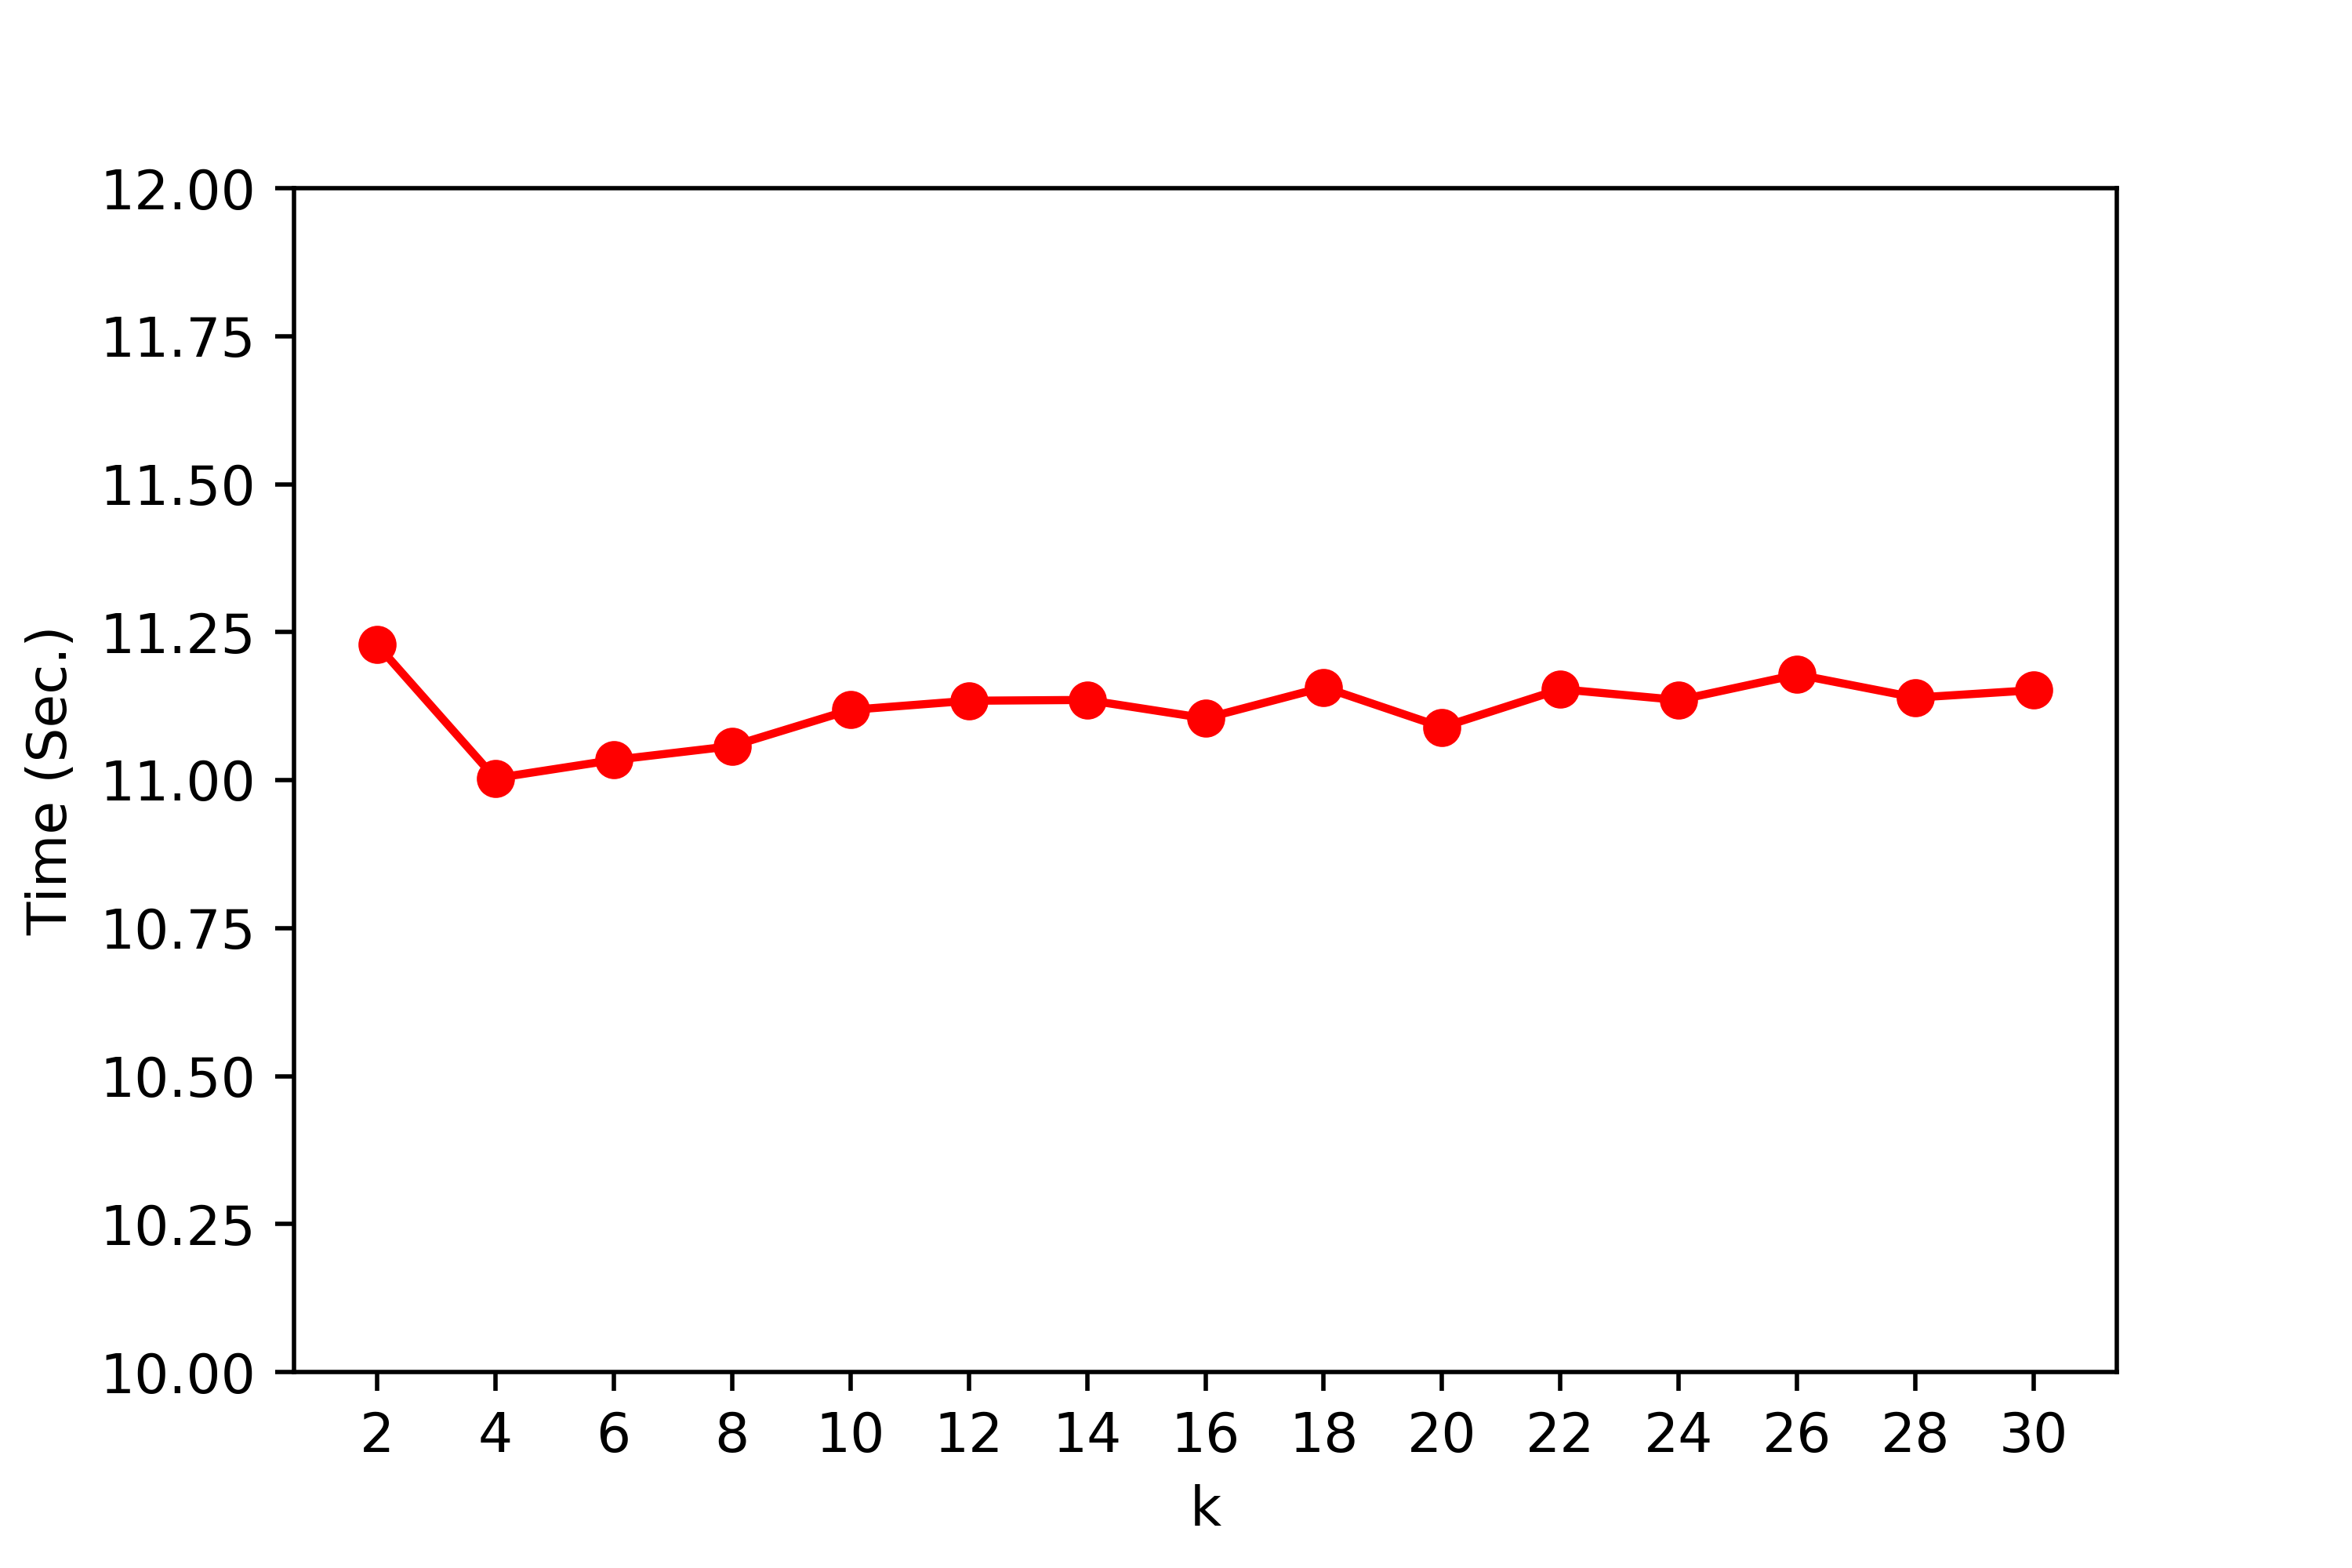
\includegraphics[scale=0.5]{KNN-LSTSVM-k}
	\caption{تاثیر پارامتر \lr{k} روی زمان آموزش روش \lr{KNN-LSTSVM}}
	\label{fig:KNN-LSTSVM-k}
\end{figure}

\newpage

\section{ارزیابی روش \lr{RKNN-TSVM}}\label{sec:5:3}
در این زیر بخش، ابتدا نحوه پیاده‌سازی و اجرای الگوریتم‌ها شرح داده شده است. سپس نحوه انتخاب پارامترهای بهینه توضیح داده شده است. در زیر بخش ، روش \lr{RKNN-TSVM} روی مجموعه داده‌های مصنوعی و واقعی به طور جامع بررسی می‌شود.

\subsection{نحوه پیاده‌سازی و اجرای الگوریتم‌ها}\label{sec:5:3:1}
نرم افزار  \lr{LightTwinSVM} برای اجرای روش \lr{TSVM} در بخش ‏\ref{sec:5:3} مورد استفاده قرار گرفته است. این نرم افزار شامل پیاده‌سازی ساده و سریع روش \lr{TSVM} می‌باشد که به عنوان بخشی از این پژوهش به طور رایگان در اختیار عموم قرار گرفته است\LTRfootnote{https://github.com/mir-am/LightTwinSVM}. روش \lr{RKNN-TSVM} و سایر روش‌ها در زبان برنامه‌نویسی پایتون نسخه \lr{3.5} پیاده‌سازی شده و همچنین الگوریتم \lr{clipDCD} و \lr{LDMDBA} در زبان برنامه‌نویسی \lr{C++} پیاده‌سازی شده است. تمامی آزمایش‌ها روی یک کامپیوتر شخصی با پردازنده \lr{Core i7 6700K}، سیستم عامل \lr{Ubuntu 16.04 LTS} و 32 گیگابایت حافظه انجام شده است. کتابخانه و نرم افزار‌های استفاده شده برای آزمایش روش \lr{RKNN-TSVM} را نشان می‌دهد. جدول \ref{tab:7} کتابخانه و نرم افزارهای استفاده شده برای آزمایش روش \lr{RKNN-TSVM} را نشان می‌دهد.


\begin{table}[!h]
	\small
	\centering
	\caption{کتابخانه و نرم افزارهای استفاده شده برای ارزیابی روش \lr{RKNN-TSVM}}
	\begin{tabular}{l c c c}
		\toprule
		% after \\: \hline or \cline{col1-col2} \cline{col3-col4} ...
		کتابخانه/نرم افزار & توضیح \\
		\midrule
		\lr{NumPy} \cite{walt2011} & اعمال جبر خطی در پایتون مانند ضرب و معکوس ماتریس \\
		\lr{SciPy} \cite{jones2014} & محاسبه فاصله و توابع آماری  \\
		\lr{Scikit-learn} \cite{pedregosa2011} & یادگیری ماشین و ارزیابی دسته‌بندها  \\
		\lr{GCC}\footnote{\lr{GNU Compiler Collection}} & کامپایلر برای زبان برنامه‌نویسی \lr{C++}   \\
		\lr{Pybind11}\footnote{\lr{https://pybind11.readthedocs.io/en/master/index.html}} & اجرای کد \lr{C++} در پایتون  \\
	
		\bottomrule
	\end{tabular}
	\label{tab:7}
\end{table}

\subsection{نحوه انتخاب پارامترها}\label{sec:5:3:2}
 همانطور که در زیر بخش \ref{sec:5:2:1} ذکر شد، عملکرد روش \lr{TSVM} و گسترش‌هایش بسیار وابسته به پارامترهای بهینه است. روش جستجوی شبکه‌ای برای انتخاب پارامترهای بهینه در آزمایش‌های بخش ‏\ref{sec:5:3} استفاده شده است. تابع \lr{RBF} به عنوان تابع هسته   $k(x_i, x_j)=\exp({-\left\|x_i - x_j\right\|^2}/\sigma^2)$ در نسخه غیر خطی بکار گرفته شده است. پارامتر تابع هسته  $\sigma$ از مجموعه  $\{2^{i} \mid i=-10,-9,\dots,2 \}$ انتخاب شده است. مقادیر بهینه پارامترهای  $c_{1}$،  $c_{2}$ و   $c_{3}$ از مجموعه   $\{2^{i} \mid i=-8,-7,\dots,2 \}$ تعیین شده است. به منظور کاهش بار محاسباتی انتخاب پارامترها،  $c_{1}=c_{2}$ و  $c_{3}=c_{4}$ در روش \lr{TBSVM}  و  $c_{2}=c_{3}$ در روش \lr{RKNN-TSVM} مساوی قرار داده شده است. همچنین مقدار بهینه پارامتر  $k$ از مجموعه   $\{2,3,\dots,15\}$ مشخص شده است.
 
\subsection{نتایج ارزیابی و بحث}\label{sec:5:3:3}
 در این زیر بخش، روش پیشنهادی (\lr{RKNN-TSVM}) روی مجموعه داده‌های مختلف مصنوعی و واقعی از نظر دقت و سرعت یادگیری بررسی می‌شود.
 
\subsubsection{مجموعه داده مصنوعی}\label{sec:5:3:3:1}
 به منظور نشان دادن برتری روش پیشنهادی نسبت به روش \lr{WLTSVM} به صورت هندسی، آزمایش روی دو مجموعه داده مصنوعی صورت گرفته است. 70 درصد نمونه‌های این مجموعه داده‌ها برای آموزش دسته‌بند به صورت تصادفی انتخاب شده است.
 
 در مثال اول، مجموعه داده مصنوعی \lr{Ripley} با 250 نمونه استفاده شده است. شکل ‏\ref{fig:WLTSVM-vs-RKNN-TSVM-R} ناحیه تصمیم روش \lr{WLTSVM} و \lr{RKNN-TSVM} را روی مجموعه داده \lr{Ripley} با تابع هسته خطی را نشان می‌دهد. همانطور که در شکل \ref{fig:WLTSVM-vs-RKNN-TSVM-R} مشخص است، روش پیشنهادی دقت بیشتری نسبت به روش \lr{WLTSVM} دارد. زیرا روش پیشنهادی به نمونه‌ها براساس فاصله نزدیک‌ترین همسایه‌هایش وزن می‌دهد. همچنین ابرصفحه‌ها در روش \lr{RKNN-TSVM} به نمونه‌های پرتراکم نزدیک‌تر دارد. 
 
 \begin{figure}[!t]
 	\centering
 	\subfloat[نسخه خطی \lr{WLTSVM} ($c=2^{3}, k=2$)]{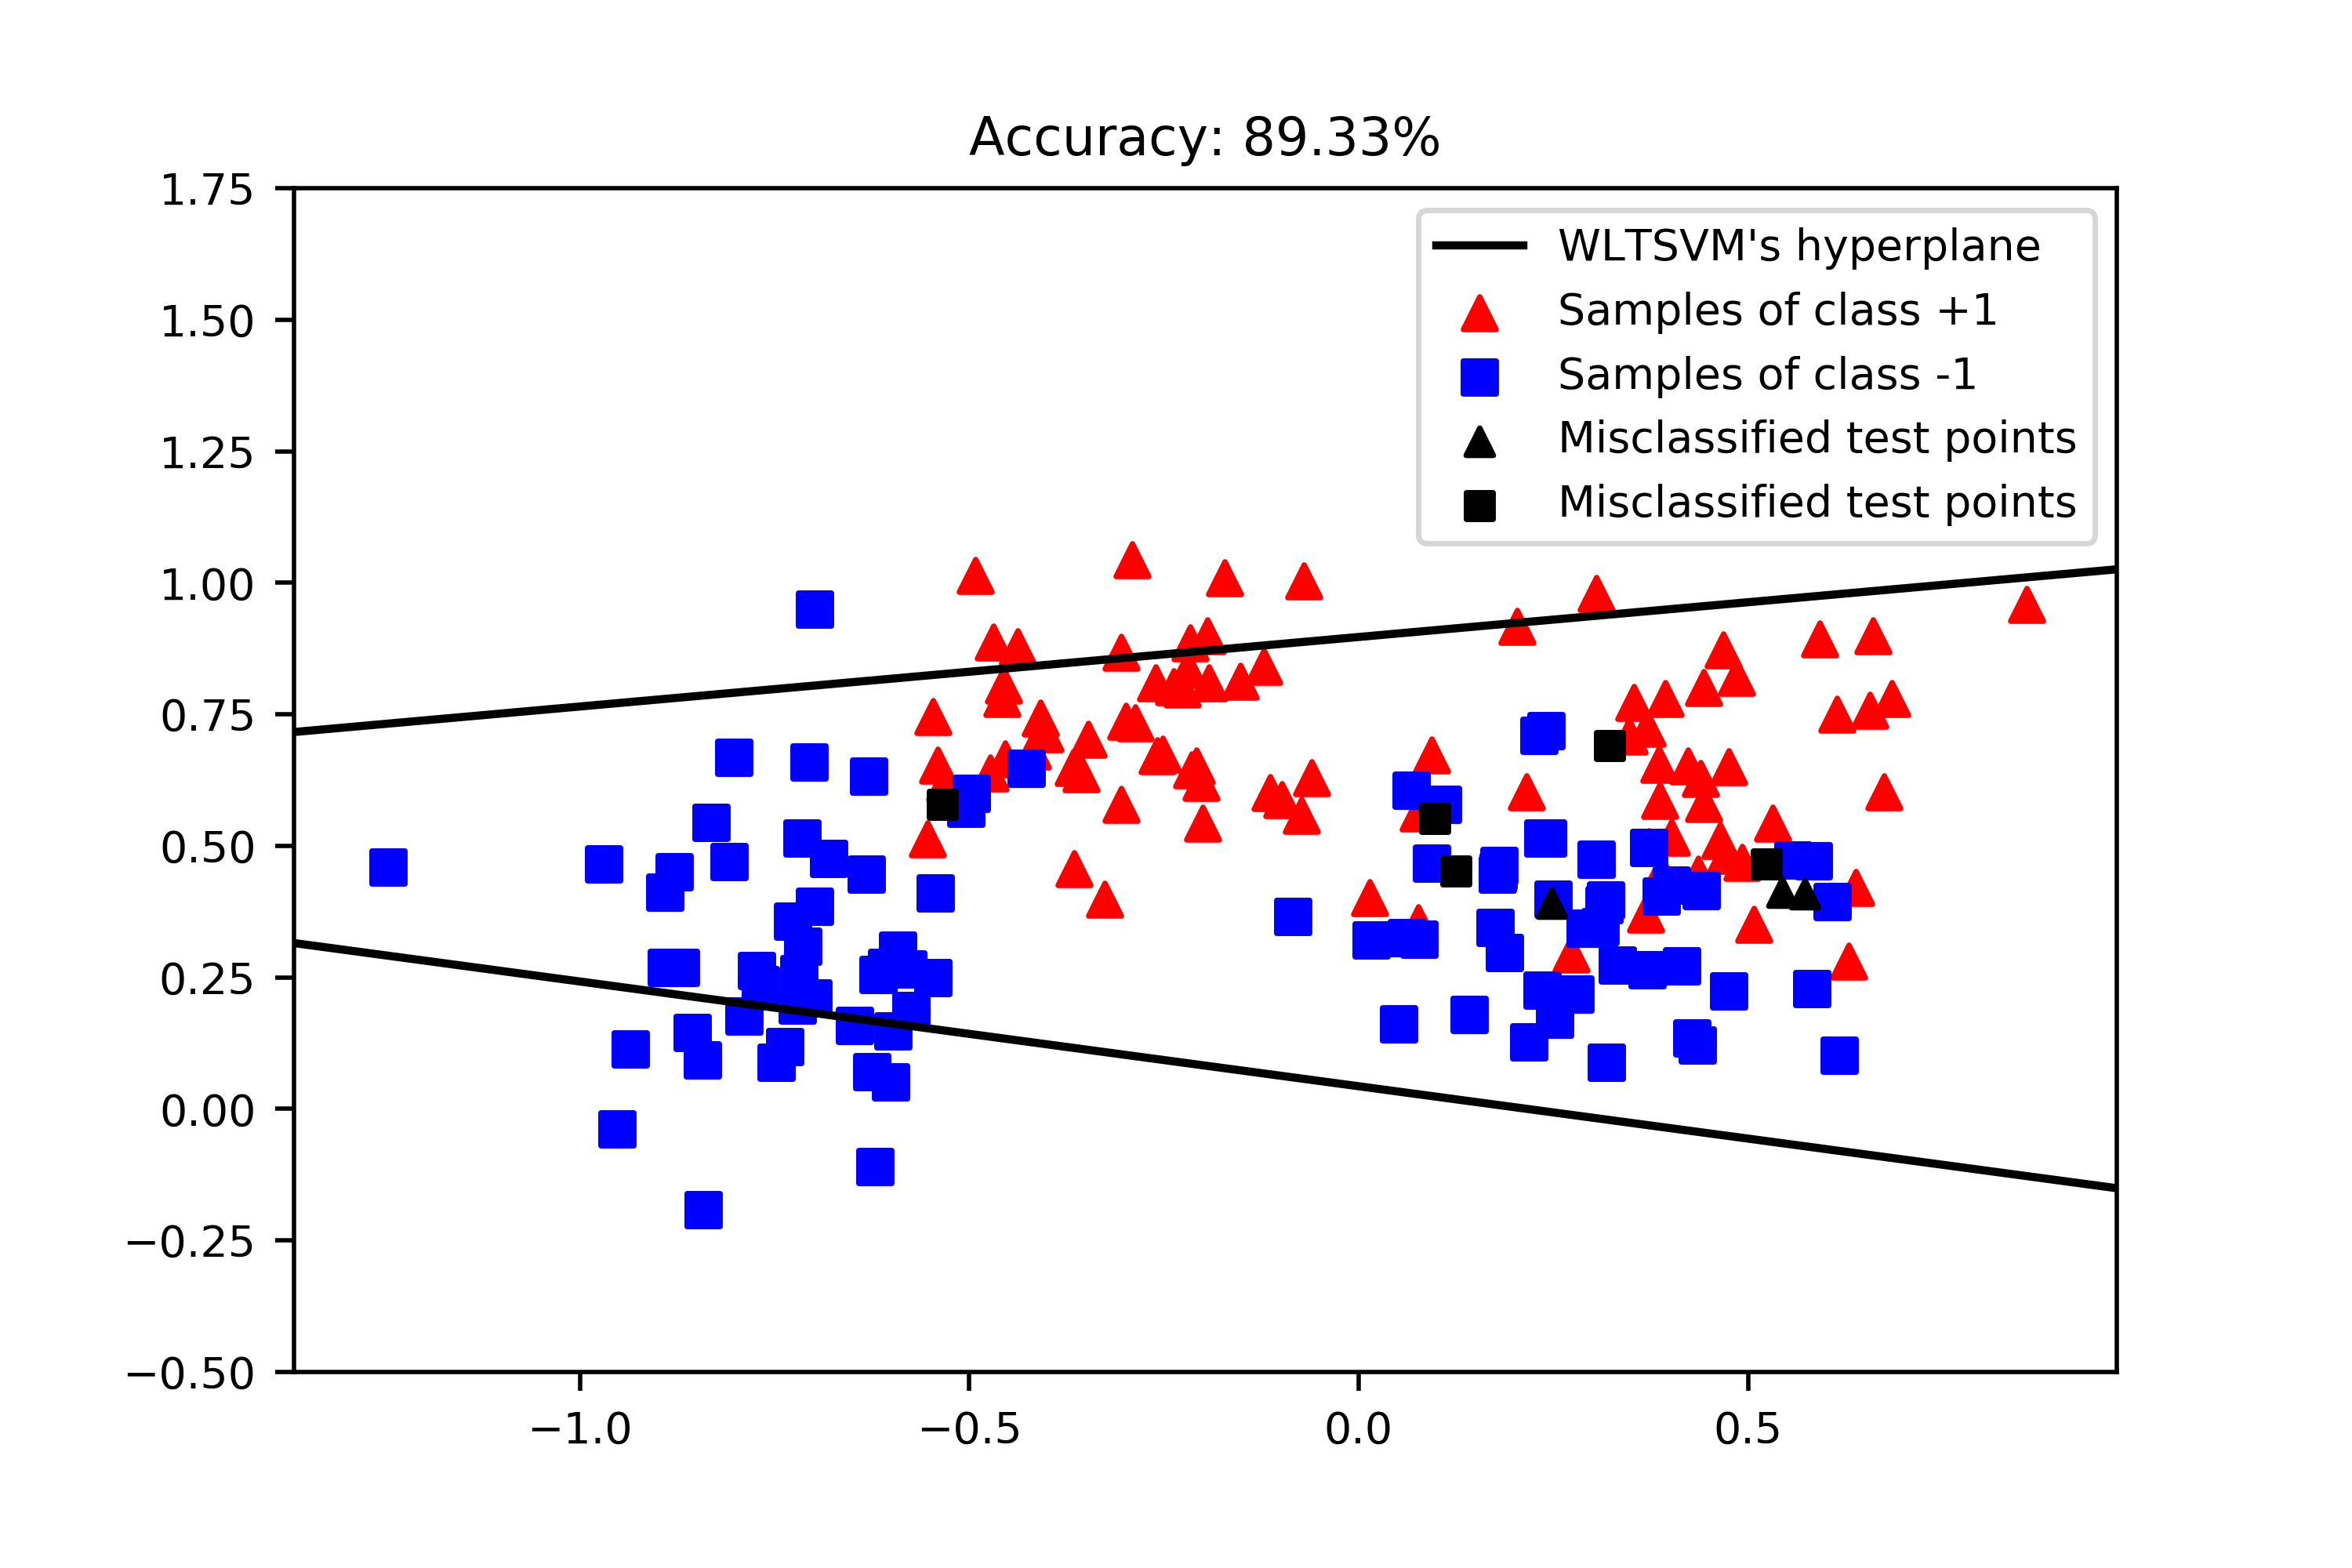
\includegraphics[width=0.5\textwidth]{WLTSVM-Ripley}}
 	\subfloat[نسخه خطی \lr{RKNN-TSVM} ($c_{1}=2^{2}, c_{2}=2^{-7}, c_{3}=2^{-2}, k=6$)]{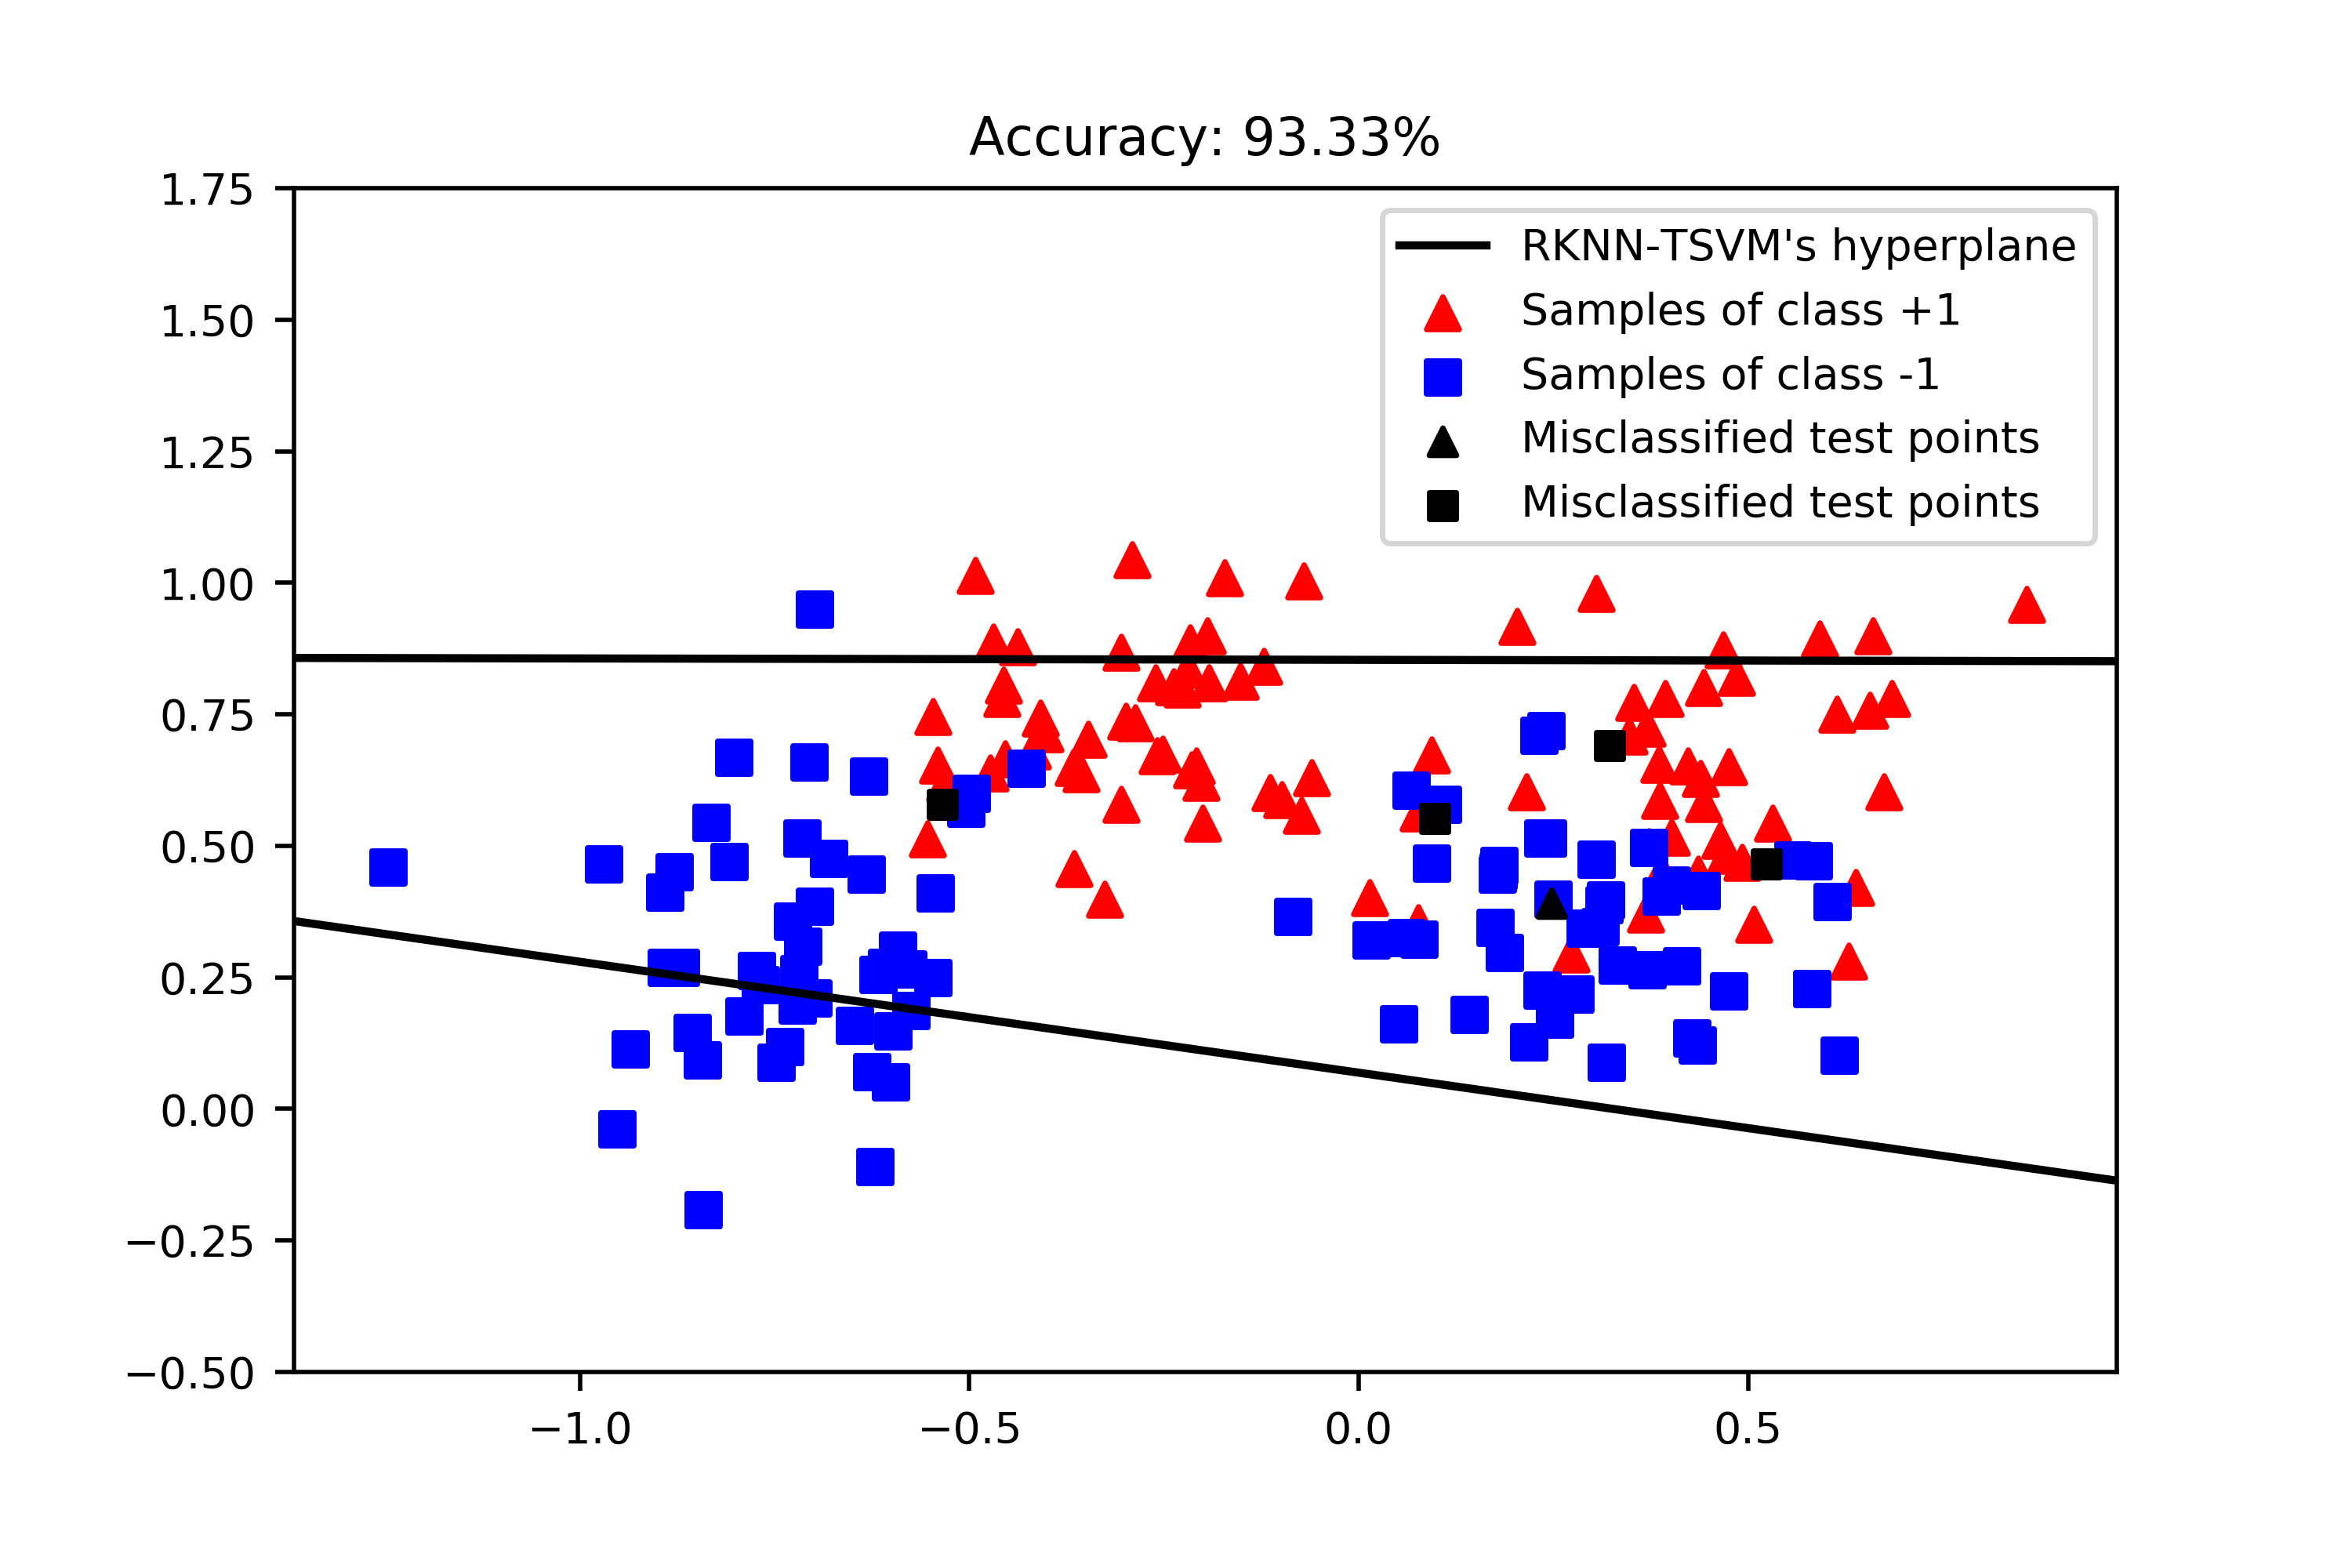
\includegraphics[width=0.5\textwidth]{RKNN-TSVM-Ripley}}
 	\caption{ناحیه تصمیم روش \lr{WLTSVM} و \lr{RKNN-TSVM} روی مجموعه داده \lr{Ripley} با تابع هسته خطی}
 	\label{fig:WLTSVM-vs-RKNN-TSVM-R}
 \end{figure}
\begin{figure}[!t]
	\centering
	\subfloat[نسخه غیر خطی \lr{WLTSVM} ($c=2^{-3}, k=8, \sigma=2^{0}$)]{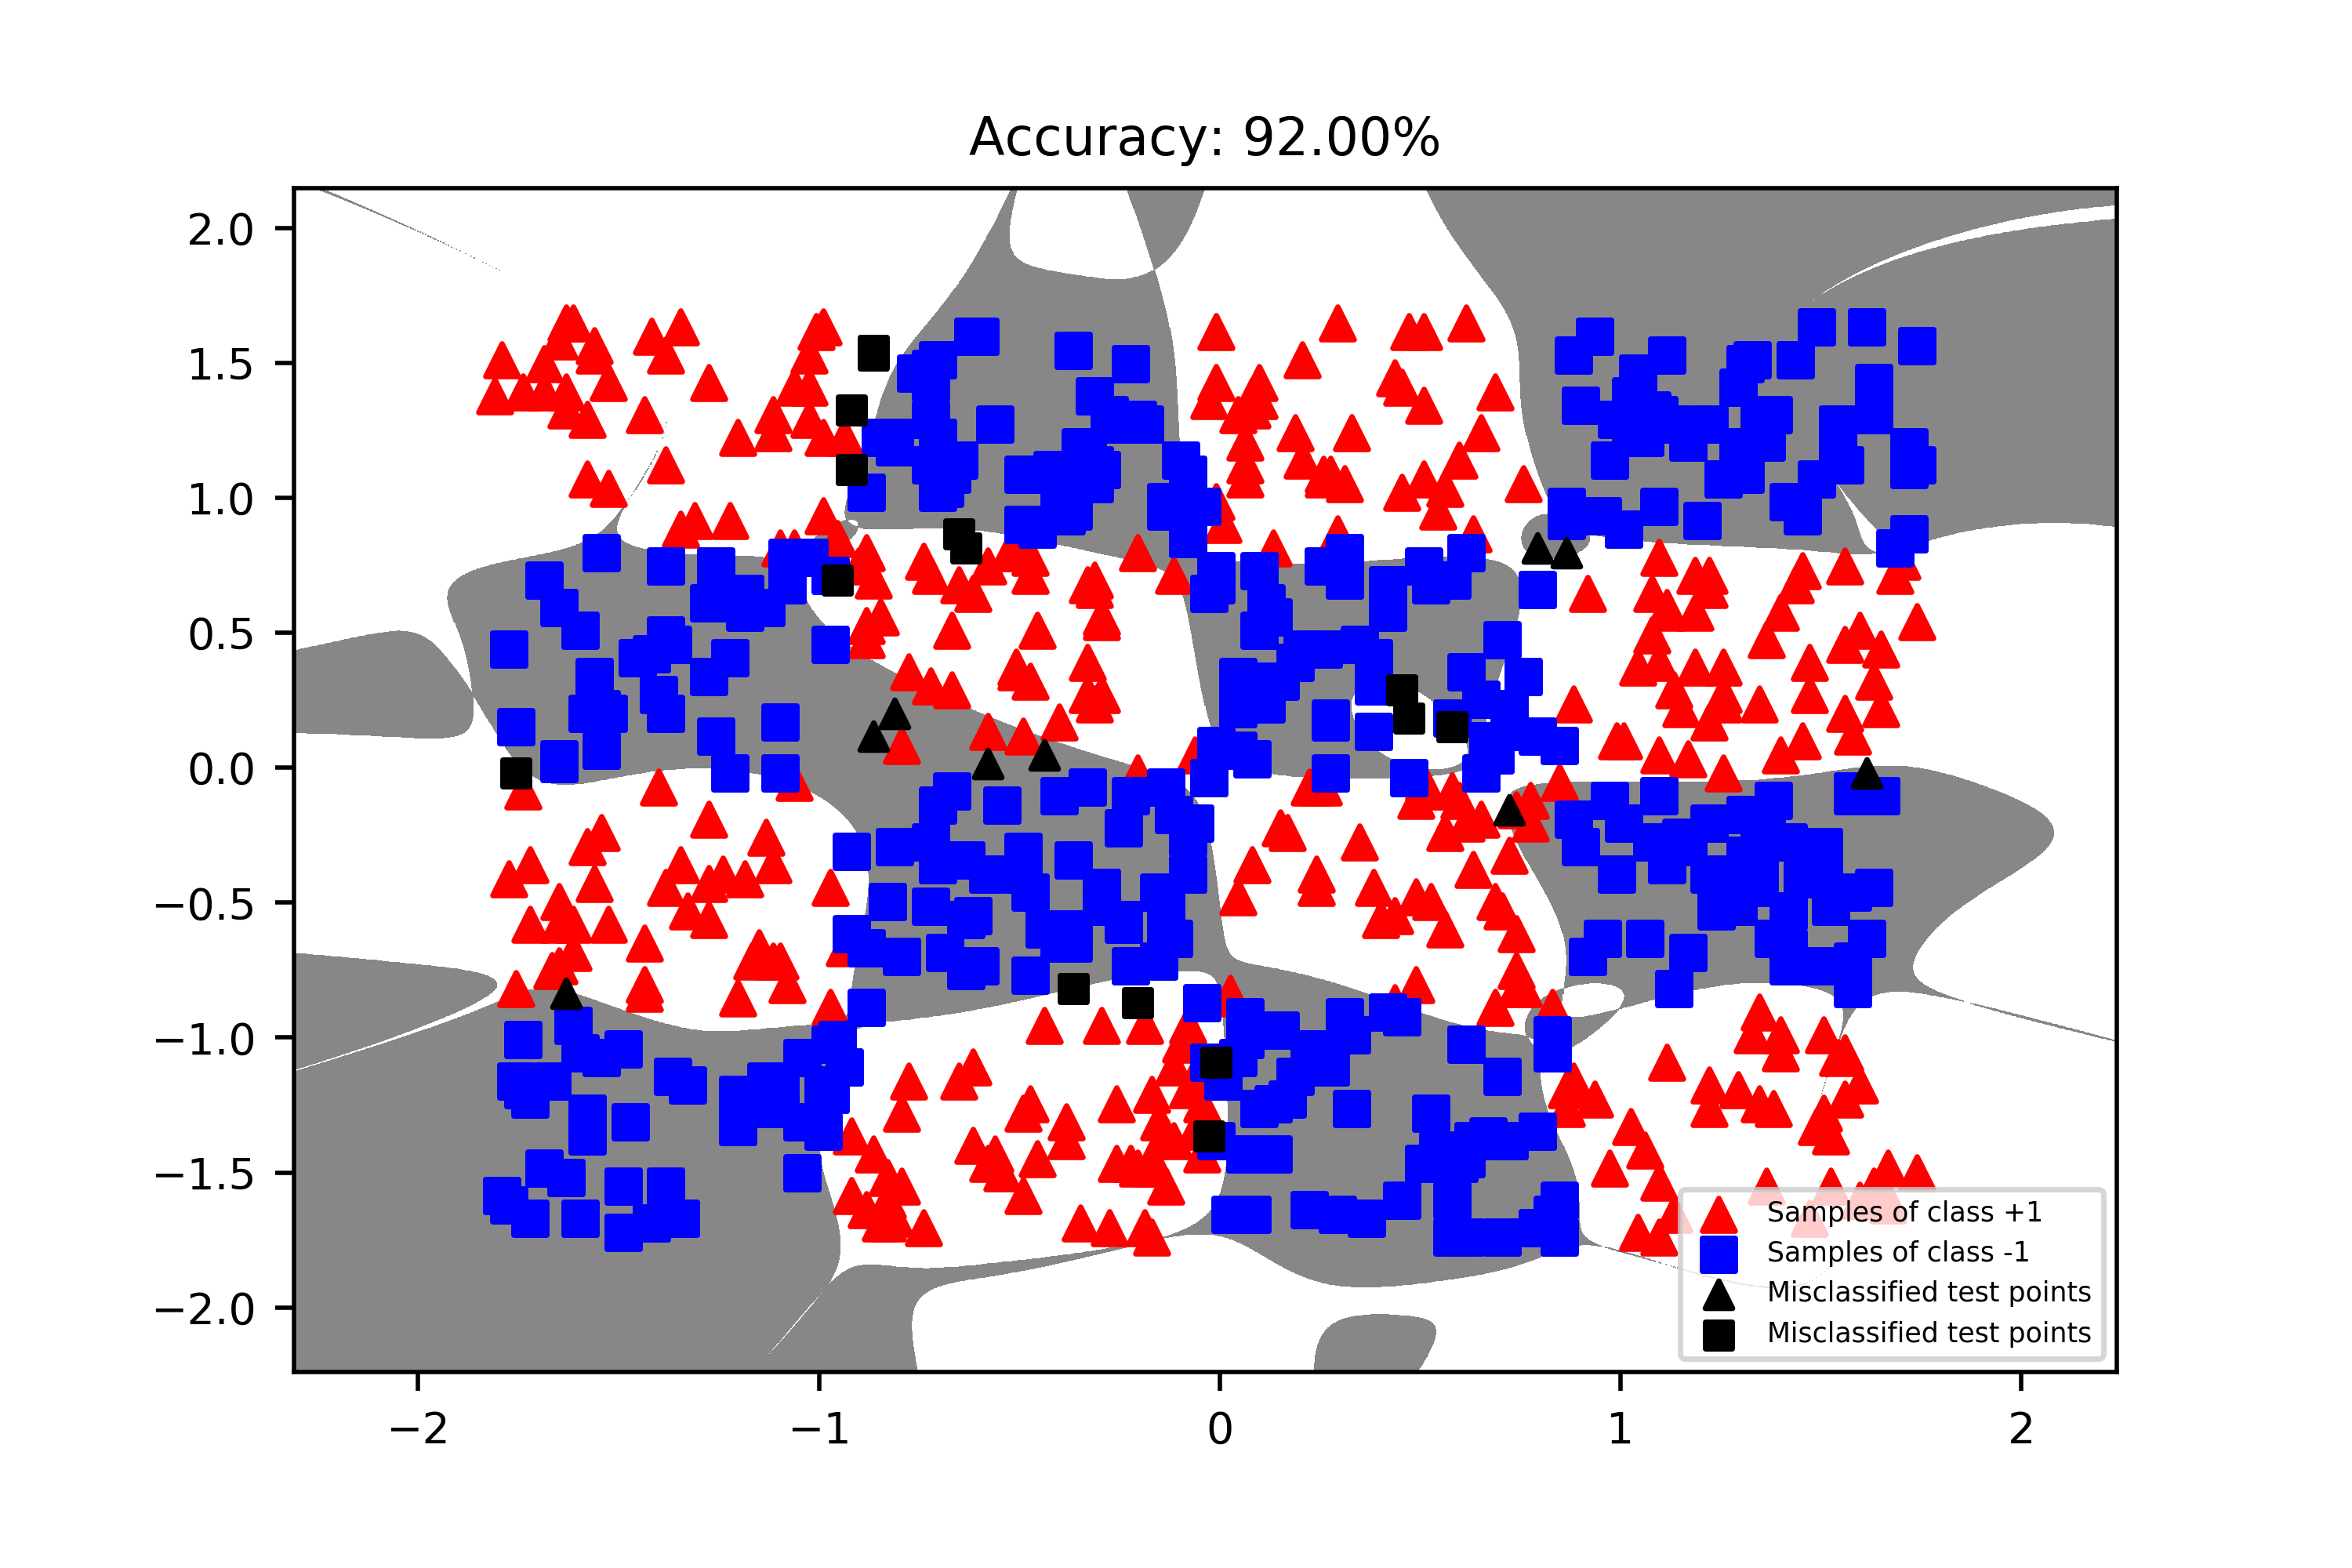
\includegraphics[width=0.5\textwidth]{WLTSVM-Check}}
	\subfloat[نسخه غیر خطی \lr{RKNN-TSVM} ($c_{1}=2^{-7}, c_{2}=2^{-6}, c_{3}=2^{-6}, k=10, \sigma=2^{1}$)]{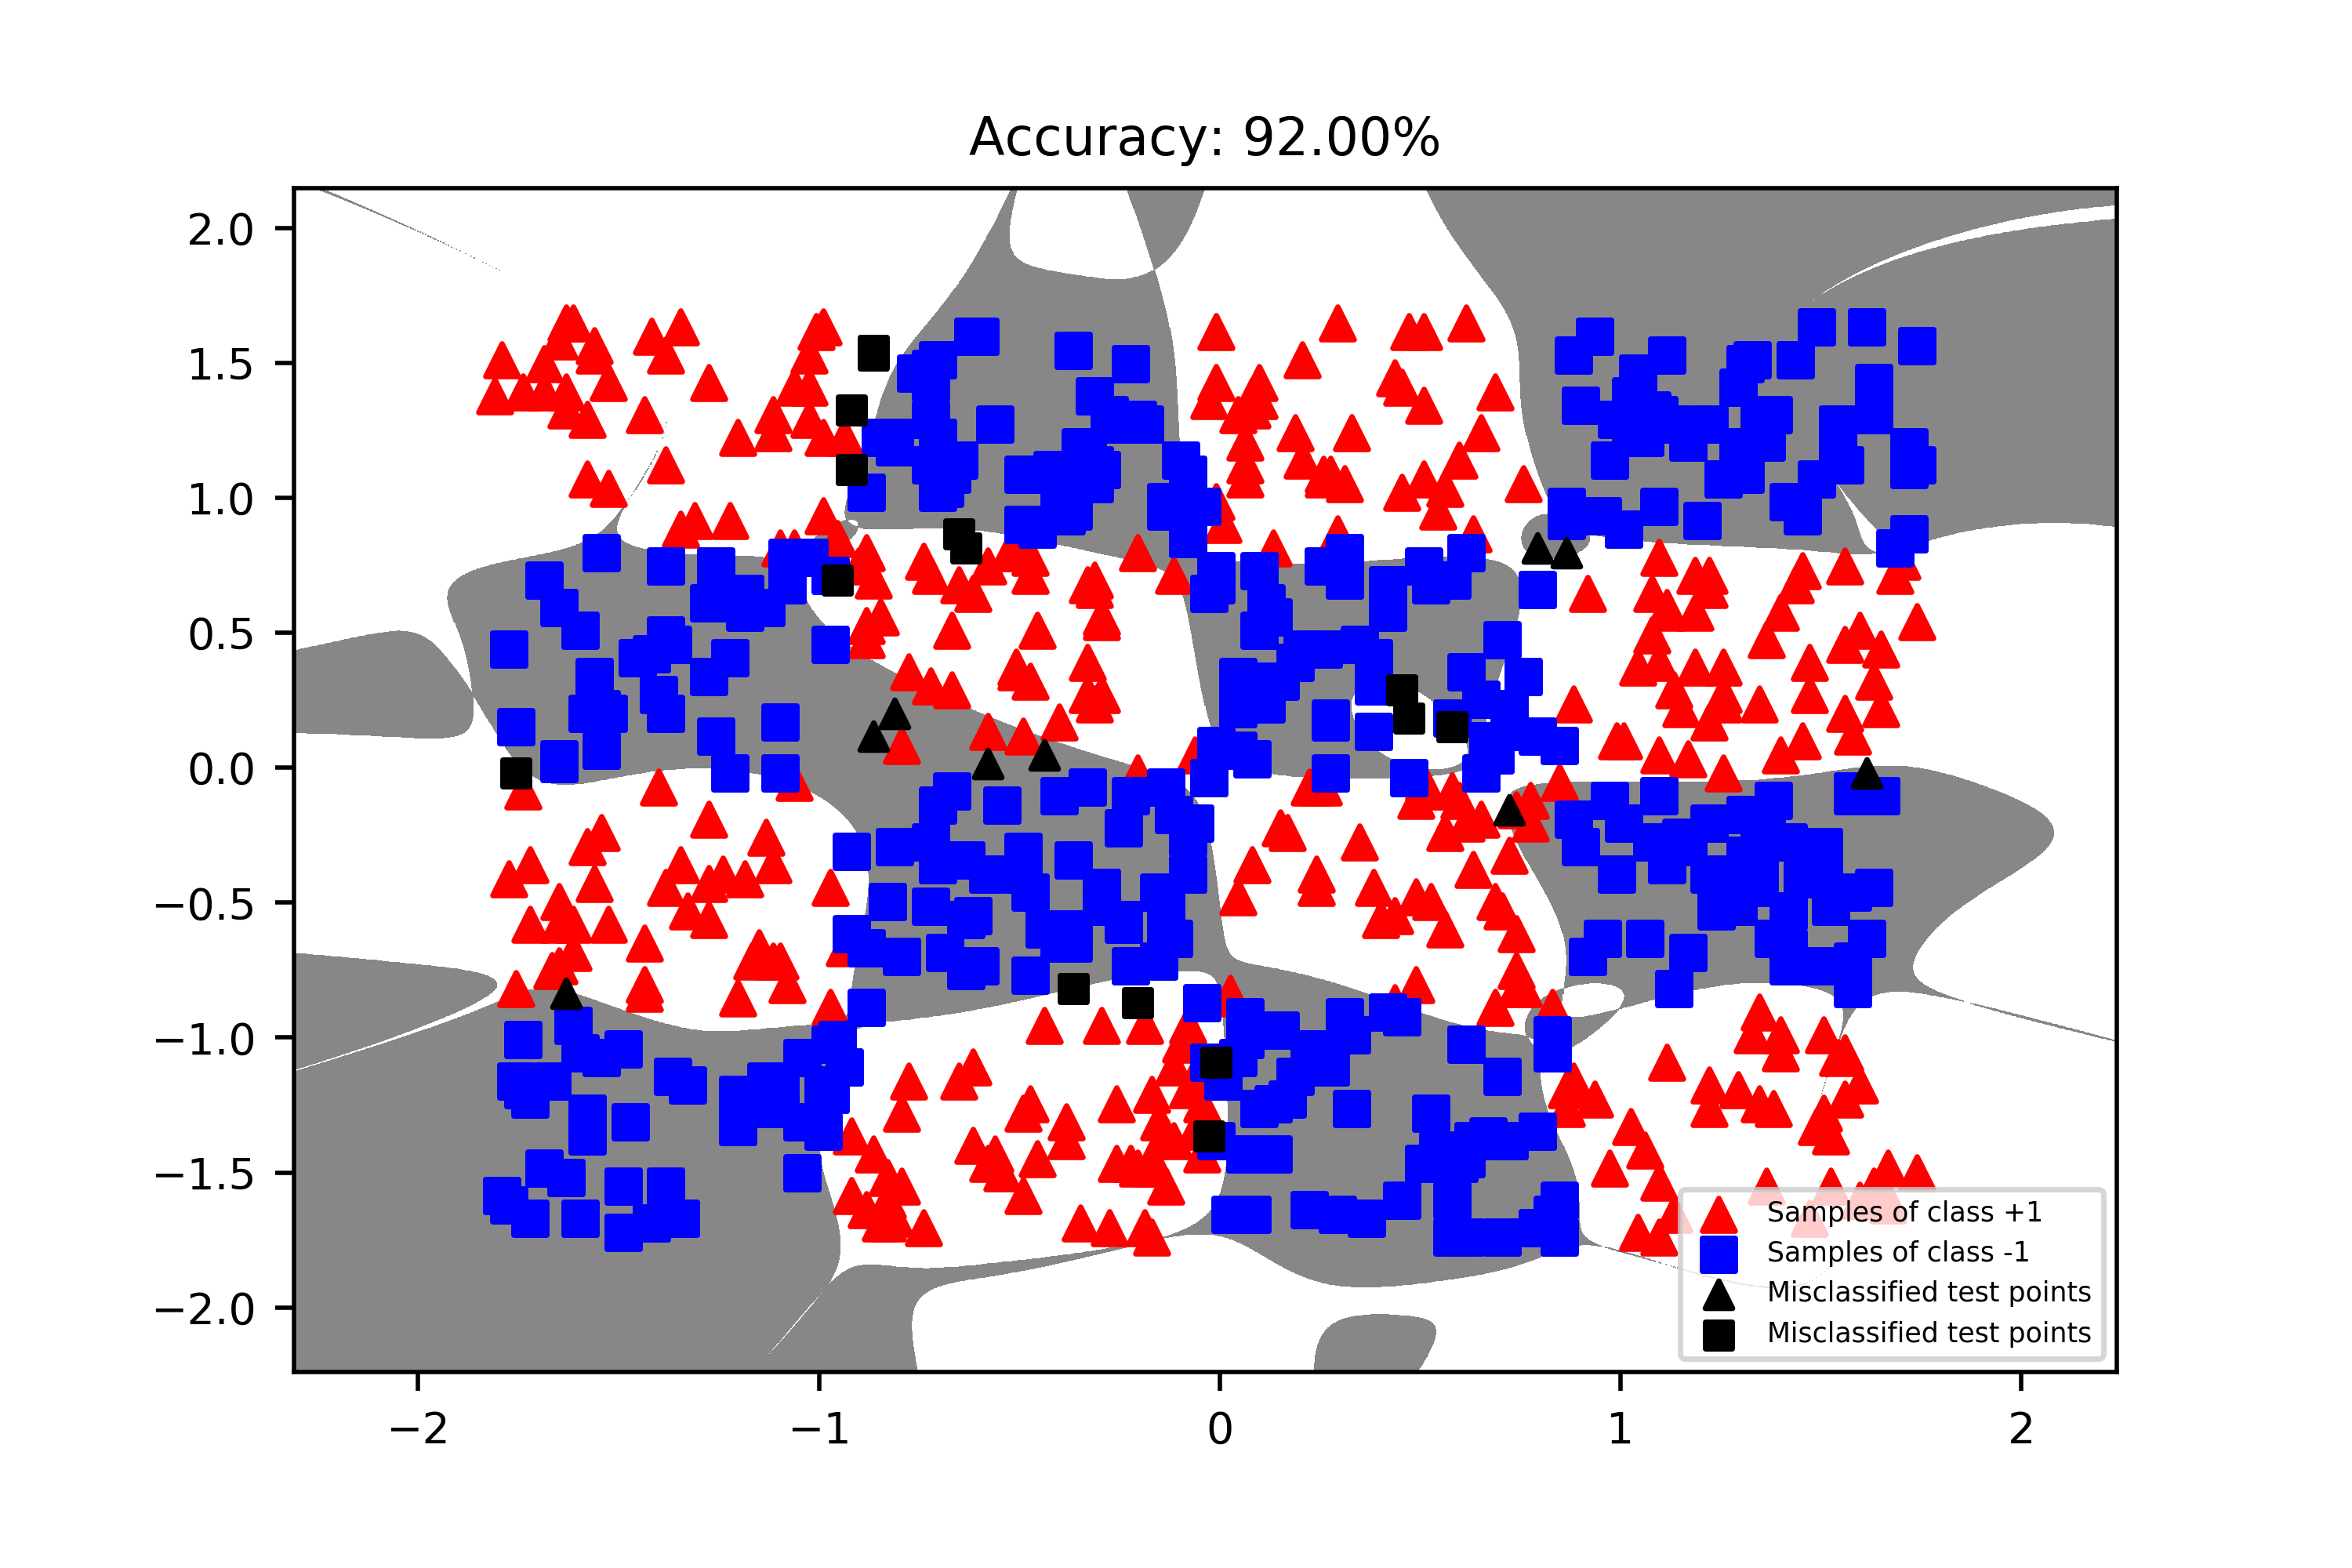
\includegraphics[width=0.5\textwidth]{RKNN-TSVM-Check}}
	\caption{ناحیه تصمیم روش  \lr{WLTSVM} و \lr{RKNN-TSVM} روی مجموعه داده \lr{Checkerboard} با تابع هسته \lr{RBF}}
	\label{fig:WLTSVM-vs-RKNN-TSVM-C}
\end{figure}

در مثال دوم، مجموعه داده مصنوعی \lr{Checkerboard} با 1000 نمونه استفاده شده است. شکل \ref{fig:WLTSVM-vs-RKNN-TSVM-C} ناحیه تصمیم روش \lr{WLTSVM} و \lr{RKNN-TSVM} را روی مجموعه داده \lr{Checkerboard} با تابع هسته \lr{RBF} را نشان می‌دهد. دقت نسخه غیر خطی روش پیشنهادی از نسخه غیر خطی روش \lr{WLTSVM} روی این مجموعه داده بیشتر است. زیرا روش پیشنهادی ریسک ساختاری را کمینه می‌کند و همچنین وزن‌دهی به نمونه‌ها براساس فاصله‌شان از نزدیک همسایه‌ها می‌باشد.

\subsubsection{مجموعه داده \lr{UCI}}\label{sec:5:3:3:2}
به منظور بررسی بیشتر عملکرد روش پییشنهادی (\lr{RKNN-TSVM})، مقایسه‌ای با روش‌های \lr{TSVM}، \lr{TBSVM} و \lr{WLTSVM} روی مجموعه داده‌های \lr{UCI} صورت گرفته است. لازم به ذکر است که تمامی مجموعه داده‌ها نرمال شده است. بطوریکه مقادیر ویژگی‌ها در بازه‌ی   $\left[0,1\right]$ قرار دارد. جدول \ref{tab:8} مشخصات این مجموعه داده‌ها را نشان می‌دهد.

\begin{table}[!t]
	\small
	\centering
	\caption{مشخصات مجموعه داده‌ها برای ارزیابی روش \lr{RKNN-TSVM}}
	\tabcolsep=0.11cm
	\begin{tabular}{l c c c c}
		\hline
		مجموعه داده & تعداد نمونه‌ها & نمونه‌های مثبت & نمونه‌های منفی & تعداد ویژگی‌ها \\
		\hline
\lr{{Australian}} & {690} & {307} & {383} & {14} \\
\lr{{Heart-Statlog}} & {270} & {120} & {150} & {13} \\
\lr{{Bupa-Liver}} & {345} & {145} & {200} & {6} \\
\lr{{WPBC}} & {198} & {47} & {151} & {33} \\
\lr{{WDBC}} & {569} & {212} & {357} & {30} \\
\lr{{Hepatitis}} & {155} & {32} & {123} & {19} \\
\lr{{Ionosphere}} & {351} & {225} & {126} & {34} \\
\lr{{Haberman}} & {306} & {225} & {81} & {3} \\
\lr{{Pima-Indian}} & {768} & {268} & {500} & {8} \\
\lr{{Fertility}} & {100} & {88} & {12} & {9} \\
\lr{{Votes}} & {435} & {267} & {168} & {16} \\
		
		\hline
	\end{tabular}
	\label{tab:8}
\end{table}

ارزیابی عملکرد روش‌ها و تنظیم کردن پارامترها با اعتبارسنج ضربدری 5 تایی انجام شده است. از این رو مجموعه داده به 5 بخش به صورت تصادفی تقسیم می‌شود و یکی از این زیربخش‌ها به عنوان نمونه‌های تست استفاده می‌گردد. فرآیند تقسیم‌بندی داده‌ها 5 بار تکرار می‌شود و میانگین این 5 بار به عنوان دقت دسته‌بند بشمار می‌رود.

دقت دسته‌بندی و زمان اجرای روش‌های \lr{TSVM}، \lr{TBSVM}، \lr{WLTSVM} و \lr{RKNN-TSVM} در جدول ذکر شده است. در اینجا دقت نشان دهنده میانگین نتایج روی داده‌های تست (به درصد) می‌باشد. زمان اجرا نیز به ثانیه است.

\begin{sidewaystable*}
	%\begin{table*}[!t]
	
	\small
	\centering
	\caption{مقایسه روش‌های \lr{TSVM}، \lr{TBSVM}، \lr{WLTSVM} و \lr{RKNN-TSVM} روی مجموعه داده‌های \lr{UCI} با تابع هسته \lr{RBF} }
	\ra{1.3} % Space between rows
	\tabcolsep=0.13cm % Adjusts column width
	%\begin{sideways}
	\begin{tabular}{p{2.70cm} \acol \tcol c \acol \tcol c \acol \tcol c \acol \tcol c \acol \tcol}
		\toprule
		
		% after \\: \hline or \cline{col1-col2} \cline{col3-col4} ...
		مجموعه داده  & \multicolumn{2}{c}{\lr{TSVM}} && \multicolumn{2}{c}{\lr{TBSVM}} && \multicolumn{2}{c}{\lr{WLTSVM}} && \multicolumn{2}{c}{\lr{RKNN-TSVM(FSA)}} && \multicolumn{2}{c}{\lr{RKNN-TSVM(LDMDBA)}} \\
		\cmidrule{2-3} \cmidrule{5-6} \cmidrule{8-9} \cmidrule{11-12} \cmidrule{14-15}
		($n\times d$) & دقت (\%) & زمان اجرا && دقت (\%) & زمان اجرا && دقت (\%) & زمان اجرا && دقت (\%) & زمان اجرا && دقت (\%) & زمان اجرا \\
		& $(c_{1}, c_{2}, \sigma)$  &  && $(c_{1}, c_{3}, \sigma)$  & && $(c, \sigma, k)$ &  && $(c_{1}, c_{2}, \sigma, k)$  &  && $(c_{1}, c_{2}, \sigma, k)$  &  \\
		\midrule
		\lr{Australian} & $87.10\pm3.09$ & $0.066$ && $87.39\pm3.39$ & $0.062$ && $86.52\pm3.53$ & $0.144$ && $87.54\pm3.65$ & $0.147$ && \textbf{$87.97\pm3.85$} & $0.226$ \\
		($690\times 14$) & ($2^{-4}, 2^{-5}, 2^{-7}$) &  && ($2^{-5}, 2^{2}, 2^{-6}$) &  && ($2^{2}, 2^{-8}, 14$) &  && ($2^{1}, 2^{-3}, 2^{-9}, 2$) &  && ($2^{-4}, 2^{-3}, 2^{-6}, 5$) & \\ 
		\lr{Heart-Statlog} & $84.81\pm2.72$ & $0.010$ && \textbf{$85.93\pm2.51$} & $0.013$ && $83.70\pm1.39$ & $0.023$ && \textbf{$85.93\pm3.01$} & $0.023$ && $85.56\pm2.16$ & $0.028$ \\
		($270\times 13$) & ($2^{0}, 2^{-1}, 2^{-10}$) &  && ($2^{0}, 2^{-3}, 2^{-10}$) &  && ($2^{0}, 2^{-7}, 12$) &  && ($2^{2}, 2^{-1}, 2^{-10}, 4$) &  && ($2^{1}, 2^{-5}, 2^{-10}, 5$) & \\ 
		\lr{Bupa-Liver} & \textbf{$74.78\pm2.35$} & $0.016$ && $73.62\pm2.13$ & $0.029$ && $73.91\pm2.05$ & $0.049$ && $73.91\pm4.30$ & $0.036$ && $73.91\pm4.58$ & $0.066$ \\
		($345\times 6$) & ($2^{1}, 2^{1}, 2^{-7}$) &  && ($2^{-2}, 2^{-7}, 2^{-5}$) &  && ($2^{0}, 2^{-6}, 10$) &  && ($2^{2}, 2^{-2}, 2^{-5}, 10$) &  && ($2^{2}, 2^{-3}, 2^{-5}, 7$) & \\ 
		\lr{WPBC} & $79.27\pm5.48$ & $0.017$ && $78.81\pm7.47$ & $0.012$ && $78.82\pm8.05$ & $0.016$ && $80.29\pm3.78$ & $0.013$ && \textbf{$80.32\pm3.98$} & $0.028$ \\
		($198\times 33$) & ($2^{-2}, 2^{-5}, 2^{-6}$) &  && ($2^{0}, 2^{-5}, 2^{-9}$) &  && ($2^{-3}, 2^{-7}, 7$) &  && ($2^{-1}, 2^{-2}, 2^{-5}, 11$) &  && ($2^{-2}, 2^{-5}, 2^{-6}, 10$) & \\ 
		\lr{WDBC} & $98.24\pm1.36$ & $0.072$ && $98.24\pm0.78$ & $0.055$ && $97.54\pm1.02$ & $0.090$ && \textbf{$98.59\pm0.70$} & $0.123$ && \textbf{$98.59\pm0.70$} & $0.157$ \\
		($569\times 30$) & ($2^{-4}, 2^{-2}, 2^{-9}$) &  && ($2^{-5}, 2^{-7}, 2^{-8}$) &  && ($2^{1}, 2^{-7}, 8$) &  && ($2^{-3}, 2^{-4}, 2^{-6}, 6$) &  && ($2^{0}, 2^{-3}, 2^{-7}, 8$) & \\ 
		\lr{Hepatitis} & $85.81\pm7.80$ & $0.004$ && $87.10\pm5.77$ & $0.004$ && $85.16\pm5.98$ & $0.012$ && $87.74\pm7.18$ & $0.017$ && \textbf{$88.39\pm6.95$} & $0.015$ \\
		($155\times 19$) & ($2^{-4}, 2^{-5}, 2^{-9}$) &  && ($2^{-5}, 2^{0}, 2^{-5}$) &  && ($2^{-5}, 2^{-7}, 11$) &  && ($2^{-4}, 2^{-3}, 2^{-6}, 7$) &  && ($2^{-4}, 2^{-3}, 2^{-6}, 3$) & \\ 
		\lr{Ionosphere} & $90.89\pm4.07$ & $0.031$ && $92.02\pm4.91$ & $0.015$ && $92.60\pm3.97$ & $0.057$ && \textbf{$93.73\pm3.45$} & $0.047$ && $93.17\pm3.87$ & $0.066$ \\
		($351\times 34$) & ($2^{-2}, 2^{-4}, 2^{-5}$) &  && ($2^{-8}, 2^{-5}, 2^{0}$) &  && ($2^{-5}, 2^{1}, 10$) &  && ($2^{-3}, 2^{1}, 2^{0}, 5$) &  && ($2^{-5}, 2^{2}, 2^{0}, 12$) & \\ 
		\lr{Haberman} & $75.46\pm5.06$ & $0.015$ && $75.82\pm3.17$ & $0.012$ && $76.11\pm7.36$ & $0.027$ && $76.77\pm5.30$ & $0.031$ && \textbf{$76.79\pm3.97$} & $0.049$ \\
		($306\times 3$) & ($2^{-2}, 2^{0}, 2^{-3}$) &  && ($2^{-3}, 2^{-4}, 2^{-3}$) &  && ($2^{0}, 2^{-6}, 11$) &  && ($2^{0}, 2^{-2}, 2^{-3}, 3$) &  && ($2^{0}, 2^{2}, 2^{-2}, 3$) & \\ 
		\lr{Pima-Indian} & $78.65\pm4.11$ & $0.089$ && $78.26\pm3.52$ & $0.059$ && $77.22\pm3.90$ & $0.193$ && $78.78\pm3.36$ & $0.191$ && \textbf{$78.91\pm2.45$} & $0.248$ \\
		($768\times 8$) & ($2^{-2}, 2^{-2}, 2^{-2}$) &  && ($2^{-1}, 2^{-6}, 2^{-2}$) &  && ($2^{2}, 2^{-3}, 10$) &  && ($2^{1}, 2^{-3}, 2^{-1}, 4$) &  && ($2^{2}, 2^{-2}, 2^{-1}, 7$) & \\ 
		\lr{Fertility} & $88.00\pm8.12$ & $0.003$ && $89.00\pm10.68$ & $0.002$ && $88.00\pm6.78$ & $0.005$ && $90.00\pm7.07$ & $0.005$ && \textbf{$91.00\pm3.74$} & $0.017$ \\
		($100\times 9$) & ($2^{-8}, 2^{-3}, 2^{-2}$) &  && ($2^{-8}, 2^{2}, 2^{1}$) &  && ($2^{-5}, 2^{1}, 2$) &  && ($2^{-3}, 2^{-1}, 2^{1}, 2$) &  && ($2^{-8}, 2^{-3}, 2^{-1}, 3$) & \\ 
		\lr{Votes} & $96.55\pm2.41$ & $0.047$ && \textbf{$97.01\pm2.00$} & $0.021$ && $96.55\pm2.91$ & $0.042$ && \textbf{$97.01\pm1.38$} & $0.040$ && \textbf{$97.01\pm1.56$} & $0.092$ \\
		($435\times 16$) & ($2^{-5}, 2^{-1}, 2^{-8}$) &  && ($2^{1}, 2^{-2}, 2^{-7}$) &  && ($2^{1}, 2^{-10}, 15$) &  && ($2^{2}, 2^{0}, 2^{-7}, 10$) &  && ($2^{2}, 2^{-5}, 2^{-9}, 11$) & \\
		&  &  && &  && &  &&  &  && & \\ 
		%\textbf{Win/draw/loss} &  &  && &  && &  &&  &  && & \\ 
		%\tiny RKNN-TSVM(LDMDBA) & 10/0/1  &  && 9/1/1 &  && 10/1/0 &  && 6/3/2 &  && & \\
		\midrule
		میانگین دقت & \multicolumn{2}{c}{$85.41$} && \multicolumn{2}{c}{$85.75$} && \multicolumn{2}{c}{$85.10$} && \multicolumn{2}{c}{$86.39$} && \multicolumn{2}{c}{\textbf{$86.51$}} \\
		\bottomrule
	\end{tabular}
	%\end{sideways}
	
	\label{tab:9}
	%\end{table*}
\end{sidewaystable*}

از جنبه دقت دسته‌بندی، روش پیشنهادی (\lr{RKNN-TSVM}) بهتر از سایر روش‌ها مانند \lr{TSVM} و \lr{WLTSVM} روی بیشتر مجموعه داده‌ها عمل کرده است. ويژگی‌های روش پیشنهادی باعث بهبود دقت شده است که در زیر توضیح داده شده است.
\begin{enumerate}
	\item روش پیشنهادی به نمونه‌ها بر اساس فاصله شان از نزدیک‌ترین همسایه‌ها وزن می‌دهد. در حالی‌که در روش  \lr{WLTSVM} صرفا  براساس شماره تعداد همسایه‌های نزدیک به نمونه وزن نسبت داده می‌شود. بطوریکه ماتریس وزن ها در روش \lr{WLTSVM} شامل مقادیر دودویی است.
	\item مشابه روش \lr{TBSVM}، روش پیشنهادی ریسک ساختاری را در مسئله بهینه سازی خود در نظر می‌گیرد. در حالی‌که روش‌های  \lr{TSVM}و  \lr{WLTSVM}ریسک تجربی را کمینه می‌کنند. به عبارت دیگر، مقادیر پارامترهای  $c_{2}$ و  $c_{3}$ دقت دسته بندی روش بهبود داده است. با این حال مقادیر این پارامتر در روش‌های \lr{TSVM} و \lr{WLTSVM} یک عدد ثابت بسیار کوچک است.
\end{enumerate}

با توجه به جدول \ref{tab:9}، نه تنها روش پیشنهادی با الگوریتم \lr{LDMDBA} از سایر روش‌های \lr{TSVM}، \lr{TBSVM} و \lr{WLTSVM} بهتر عمل کرده است، بلکه نسبت به روش پیشنهادی با الگوریتم \lr{FSA} نیز دقت بیشتری دارد. هدف از بکارگیری الگوریتم \lr{LDMDBA} بهبود سرعت آموزش روش ‍پیشنهادی بوده است. با این حال این الگوریتم دقت دسته‌بندی روش ‍پیشنهادی را هم افزایش داده است.

از جنبه زمان اجرا و سرعت آموزش، روش \lr{TSVM} از روش پیشنهادی و \lr{WLTSVM} سریع‌تر است. زیرا روش فقط دو مسئله دوگان را حل می‌کند. در حالی‌که در روش پیشنهادی و \lr{WLTSVM} علاوه بر حل کردن دو مسئله دوگان، نزدیک‌ترین همسایه‌های تمام نمونه‌ها باید محاسبه گردد. به منظور بهبود مرتبه زمانی روش پیشنهادی (\lr{RKNN-TSVM})، الگوریتم \lr{LDMDBA} برای ساخت گراف نزدیک‌ترین همسایه استفاده شده است. در بخش \ref{sec:5:3:3:5}، سرعت آموزش روش پیشنهادی بر روی مجموعه داده‌های بزرگ بررسی شده است.

شکل \ref{fig:RKNN-TSVM-k} تاثیر مقدار پارامتر $k$ روی زمان آموزش روش پیشنهادی با الگوریتم \lr{FSA} و \lr{LDMDBA} روی مجموعه داده \lr{Pima-Indian} را نشان می‌دهد. همانطور که در شکل \ref{fig:RKNN-TSVM-k} مشخص است، زمان آموزش روش پیشنهادی با افزایش مقدار $k$ بیشتر می‌شود. با این حال روش پیشنهادی با الگوریتم \lr{LDMDBA} به طور قابل توجه‌ای از الگوریتم \lr{FSA} برای هر یک از مقادیر $k$ سریع‌تر است.

\begin{figure}[!t]
	\centering
	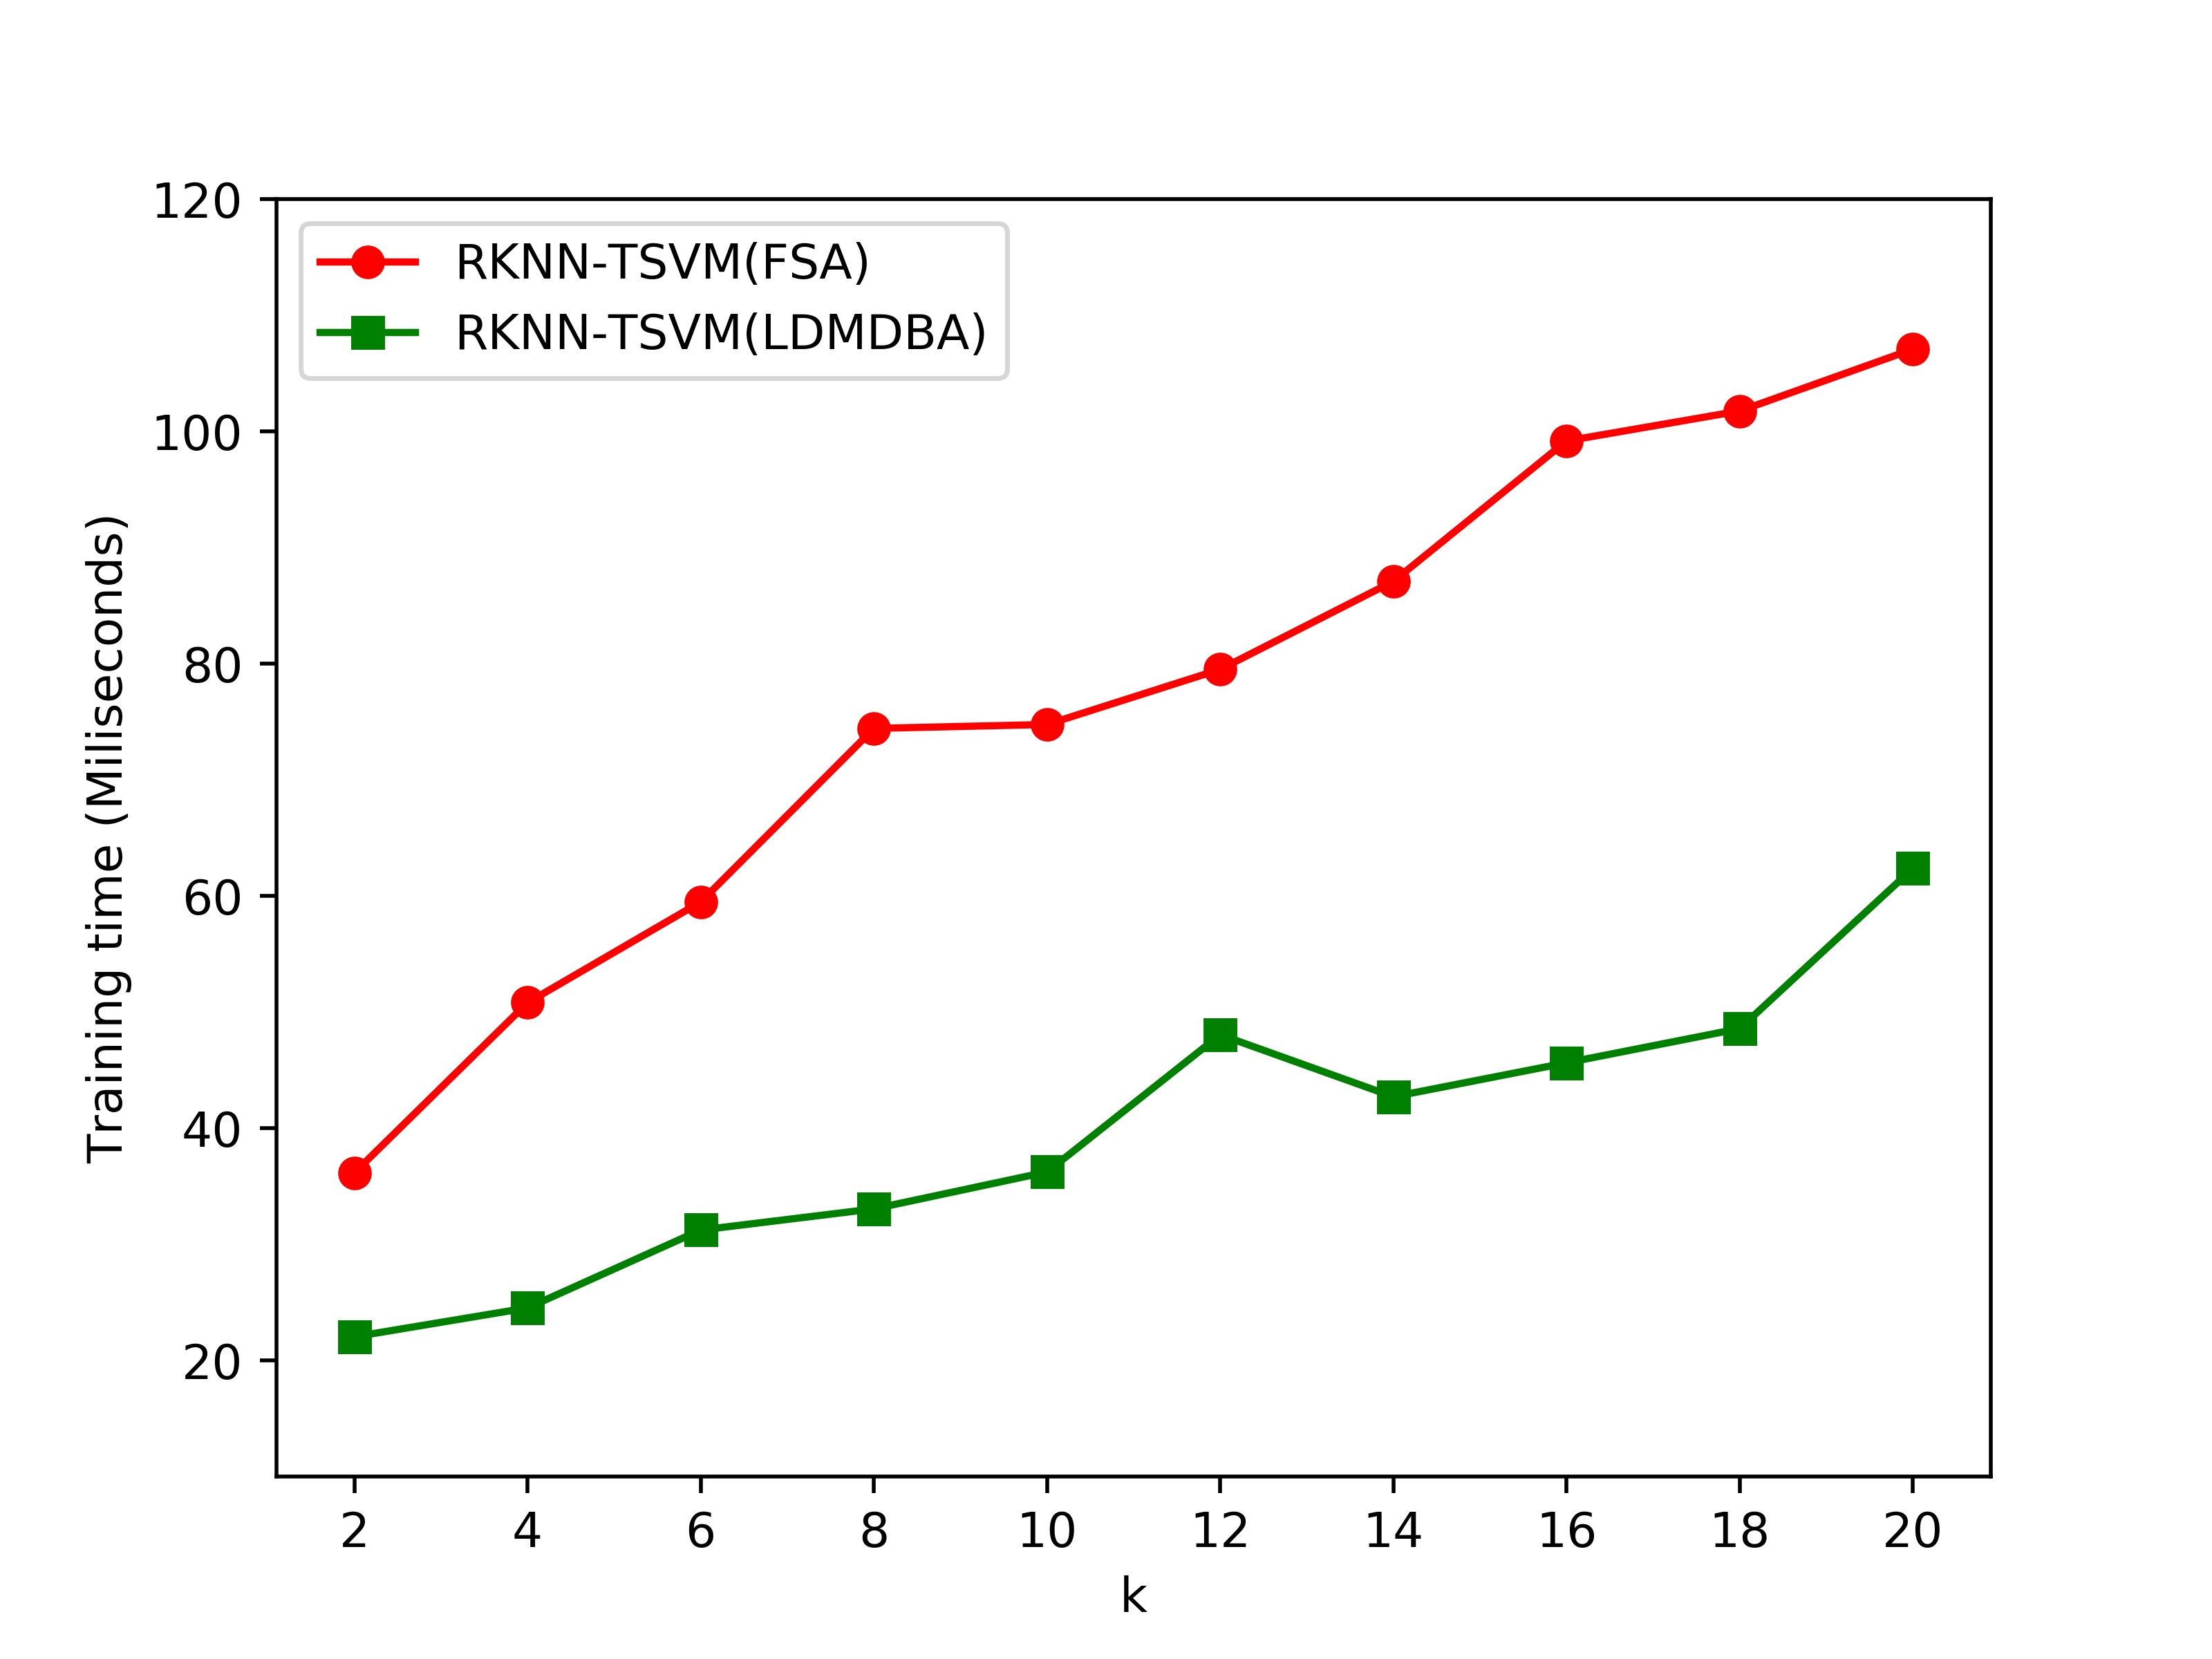
\includegraphics[scale=0.5]{RKNN-TSVM-k}
	\caption{تاثیر پارامتر $k$ روی زمان آموزش روش \lr{RKNN-TSVM} روی مجموعه داده \lr{Pima-Indian} }
	\label{fig:RKNN-TSVM-k}
\end{figure}

\subsubsection{بررسی آماری}\label{sec:5:3:3:3}
به منظور تحلیل آماری عملکرد پنج دسته‌بند روی مجموعه داده‌های \lr{UCI}، آزمون فریدمن بکار گرفته شده است (نحوه محاسبه این آزمون آماری در بخش \ref{sec:5:2:3:1} بیان شده است.). بدین منظور میانگین رتبه پنج روش براساس دقت محاسبه شده و در جدول نمایش داده شده است. ابتدا فرض گرفته می‌شود که بر اساس فرضیه صفر تمام دسته‌بندها یکسان هستند.

\begin{table}[!t]
	\centering
	\caption{میانگین رتبه براساس دقت (ارزیابی \lr{RKNN-TSVM})}
	\ra{1.3} % Space between rows
	\tabcolsep=0.10cm
	\begin{tabular}{c c c c c c c c c c c c c}
		\toprule
		% after \\: \hline or \cline{col1-col2} \cline{col3-col4} ...
		مجموعه داده  & \lr{TSVM }& \lr{TBSVM} & \lr{WLTSVM} & \lr{RKNN-TSVM(FSA)} & \lr{RKNN-TSVM(LDMDBA) }\\
		\midrule
\lr{Australian} & 4 & 3 & 5 & 2 & 1\\ 
\lr{Heart-Statlog} & 4 & $1.5$ & 5 & $1.5$ & 3\\ 
\lr{Bupa-Liver} & 1 & 5 & 3 & 3 & 3\\ 
\lr{WPBC} & 3 & 5 & 4 & 2 & 1\\ 
\lr{WDBC} & $3.5$ & $3.5$ & 5 & $1.5$ & $1.5$\\ 
\lr{Hepatitis} & 4 & 3 & 5 & 2 & 1\\ 
\lr{Ionosphere} & 5 & 4 & 3 & 1 & 2\\ 
\lr{Haberman} & 5 & 4 & 3 & 2 & 1\\ 
\lr{Pima-Indian} & 3 & 4 & 5 & 2 & 1\\ 
\lr{Fertility} & $4.5$ & 3 & $4.5$ & 2 & 1\\ 
\lr{Votes} & $4.5$ & 2 & $4.5$ & 2 & 2\\ 
میانگین رتبه & $3.77$ & $3.45$ & $4.27$ & $1.91$ & \textbf{$1.59$} \\ 
		\bottomrule
	\end{tabular}
	
	\label{tab:10}
\end{table}

بعد از انجام آزمون آماری فریدمن، مقادیر $\chi^2_F = 24.636$ و $F_F = 12.723$ بدست آمده است. با در نظرگرفتن 5 دسته‌بند و 11 مجموعه داده، $F_F$ از توزیع $F$ با (4, 40) درجه آزادی پیروی می‌کند. مقادیر ویژه $F(4,40)$ برای سطوح معناداری $0.25$، $0.1$ و $0.05$ به ترتیب برابر با $1.40$، $2.09$ و $2.61$ است. مقدار $F_F$ به طور قابل توجه‌ای بیشتر از مقدار ويژه است. بنابر با توجه به نتایج آزمون آماری، فرضیه صفر رد می‌شود. در نتیجه تفاوت معنادار و قابل توجه‌ای بین ۵ دسته‌بند وجود دارد. همچنین جدول \ref{tab:10} نشان می‌دهد که روش پیشنهادی (\lr{RKNN-TSVM}) بهتر از سایر روش ها عمل کرده است. زیرا میانگین رتبه روش پیشنهادی در میان سایر روش‌ها کمترین است.

\subsubsection{بررسی حساسیت روش \lr{RKNN-TSVM} به پارامترها}\label{sec:5:3:3:4}
به منظور دست‌یابی به دقت بهتر، انتخاب پارامترهای بهینه برای روش پیشنهادی اهمیت زیادی دارد. آزمایش روی دو مجموعه داده \lr{Australian} و \lr{Hepatitis} صورت گرفته است تا حساسیت روش پیشنهادی به پارامترهای $c_{1}$، $c_{2}$ و $k$ بررسی شود.

\begin{figure}[!t]
	\centering
	\subfloat[مجموعه داده \lr{Australian}]{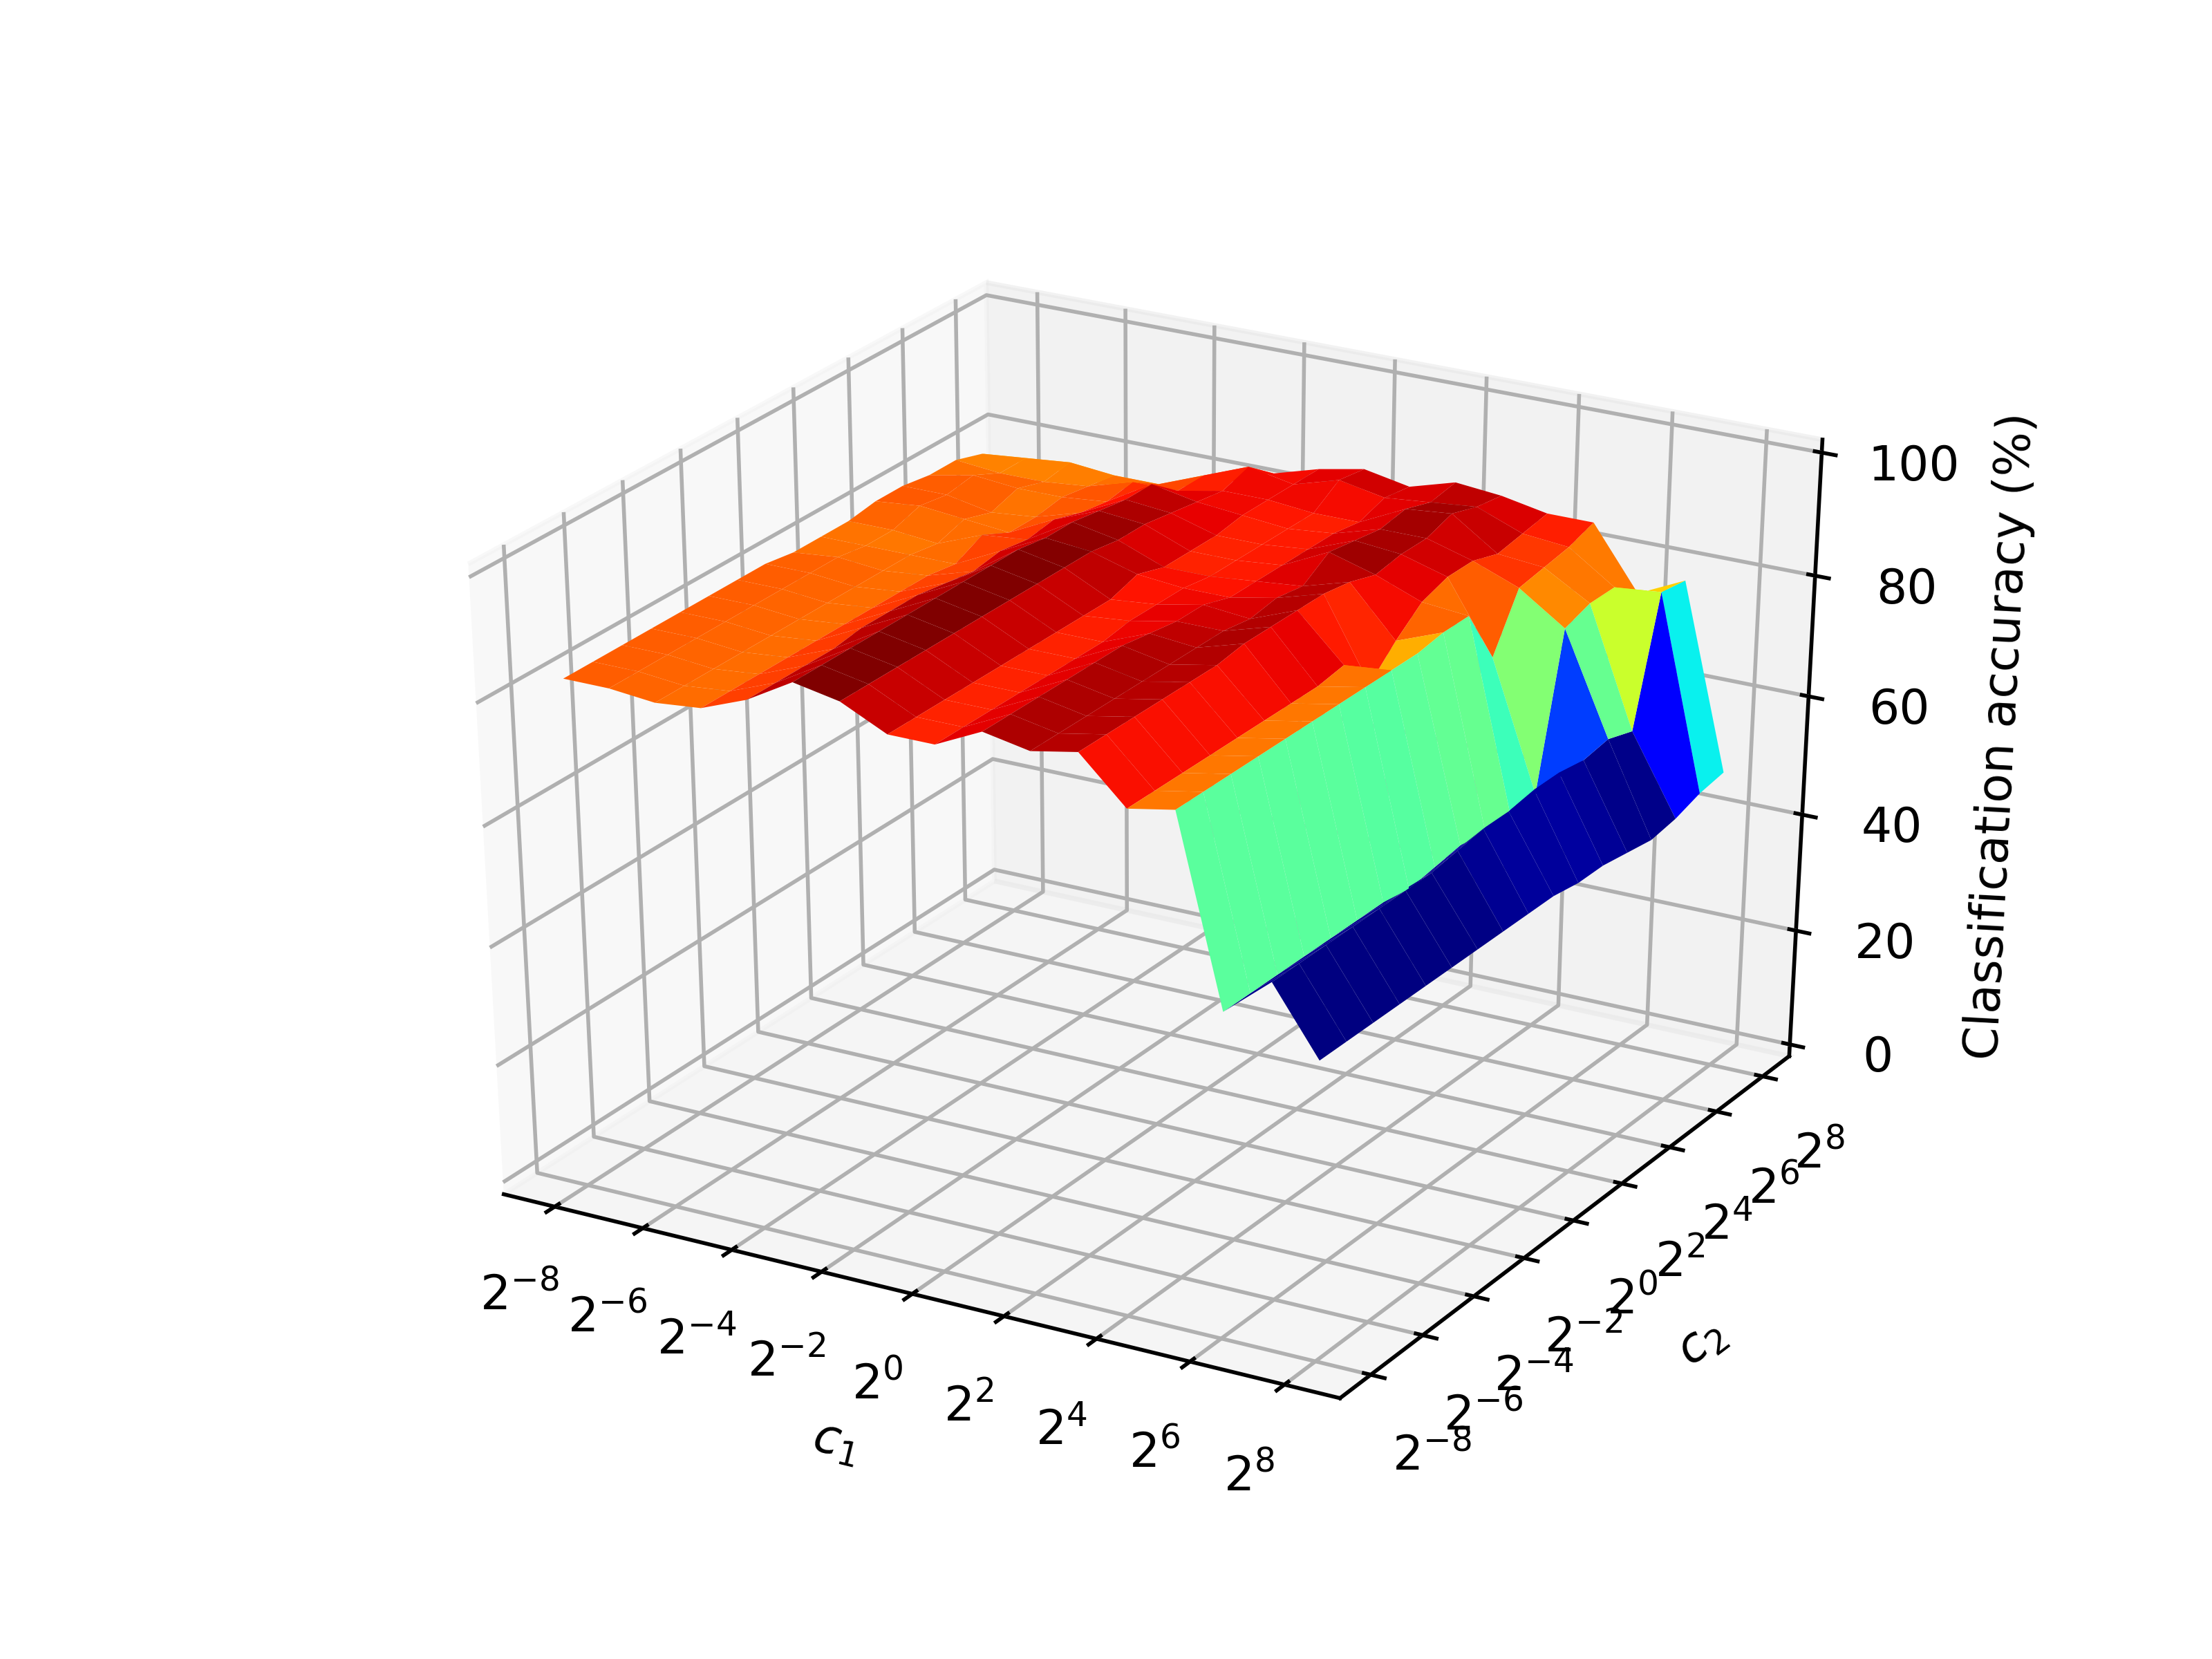
\includegraphics[width=0.5\textwidth]{RKNN-TSVM-Aust-C_1_2}}
	\subfloat[مجموعه داده \lr{Hepatitis}]{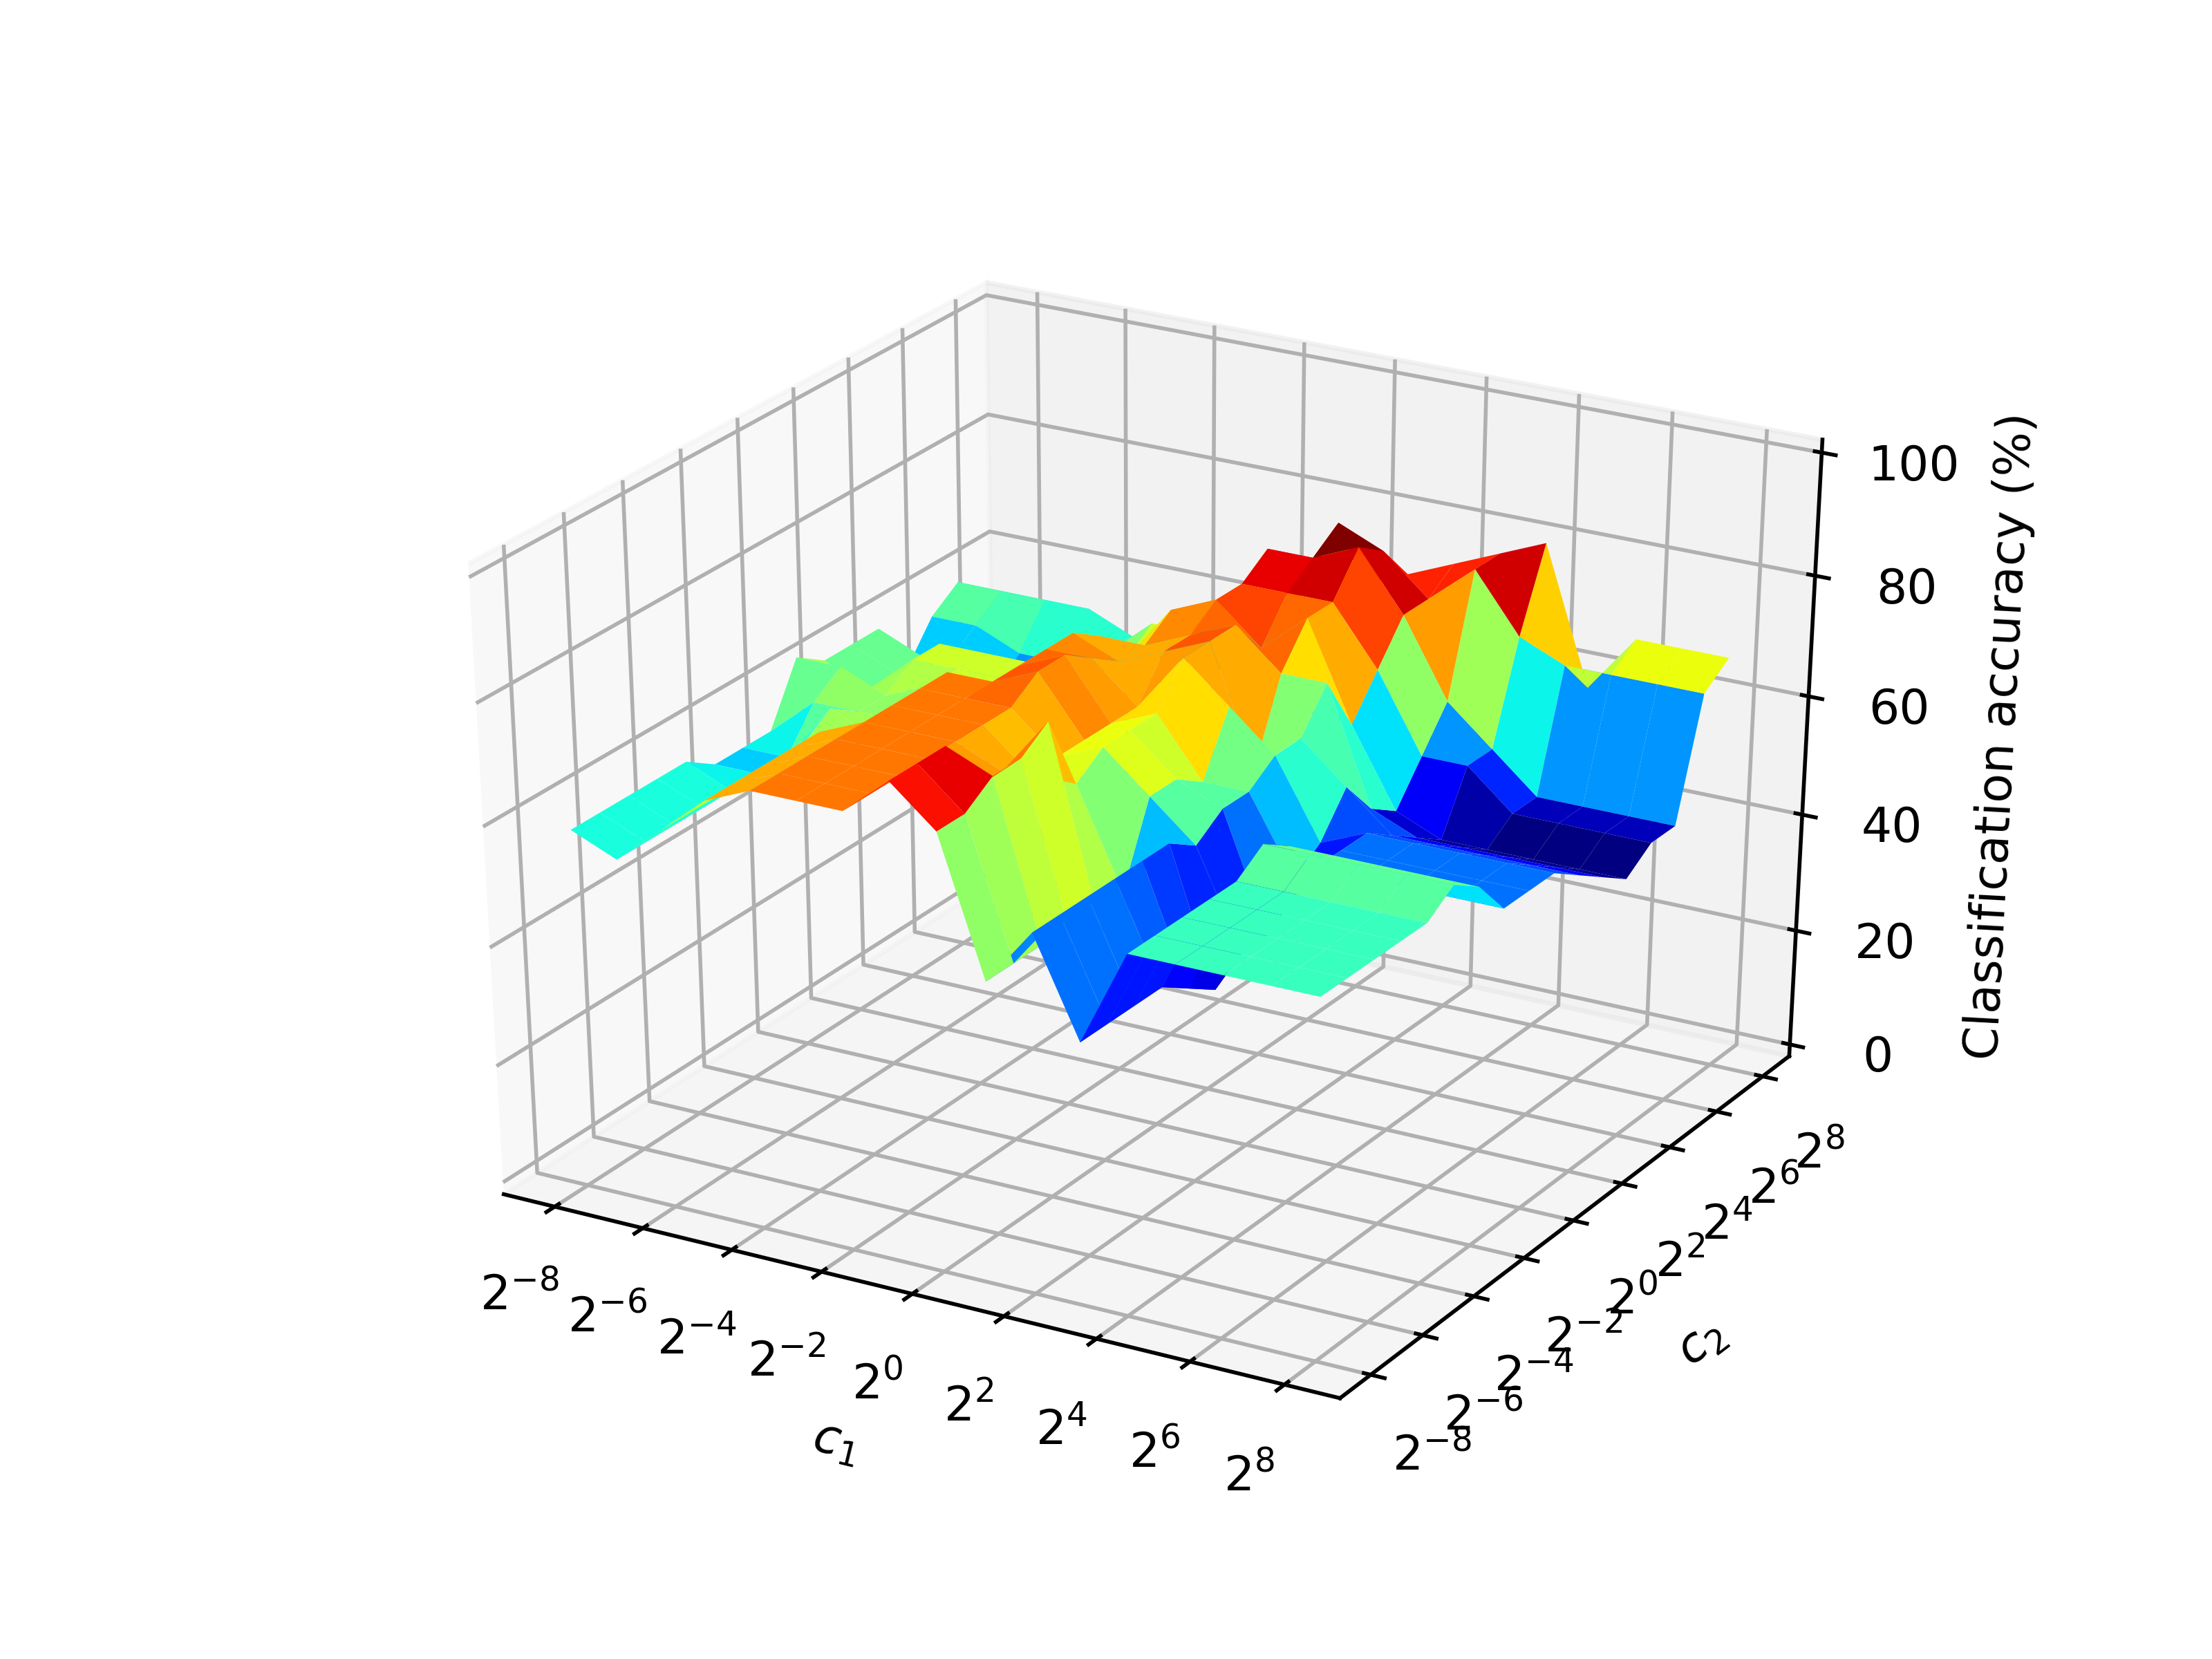
\includegraphics[width=0.5\textwidth]{RKNN-TSVM-Hep-C_1_2}}
	\caption{عملکرد نسخه خطی روش \lr{RKNN-TSVM} روی پارامترهای مختلف $c_{1}$ و $c_{2}$}
	\label{fig:RKNN-TSVM-Aust-Hep-C_1_2}
\end{figure}
\begin{figure}[!t]
	\centering
	\subfloat[مجموعه داده \lr{Australian}]{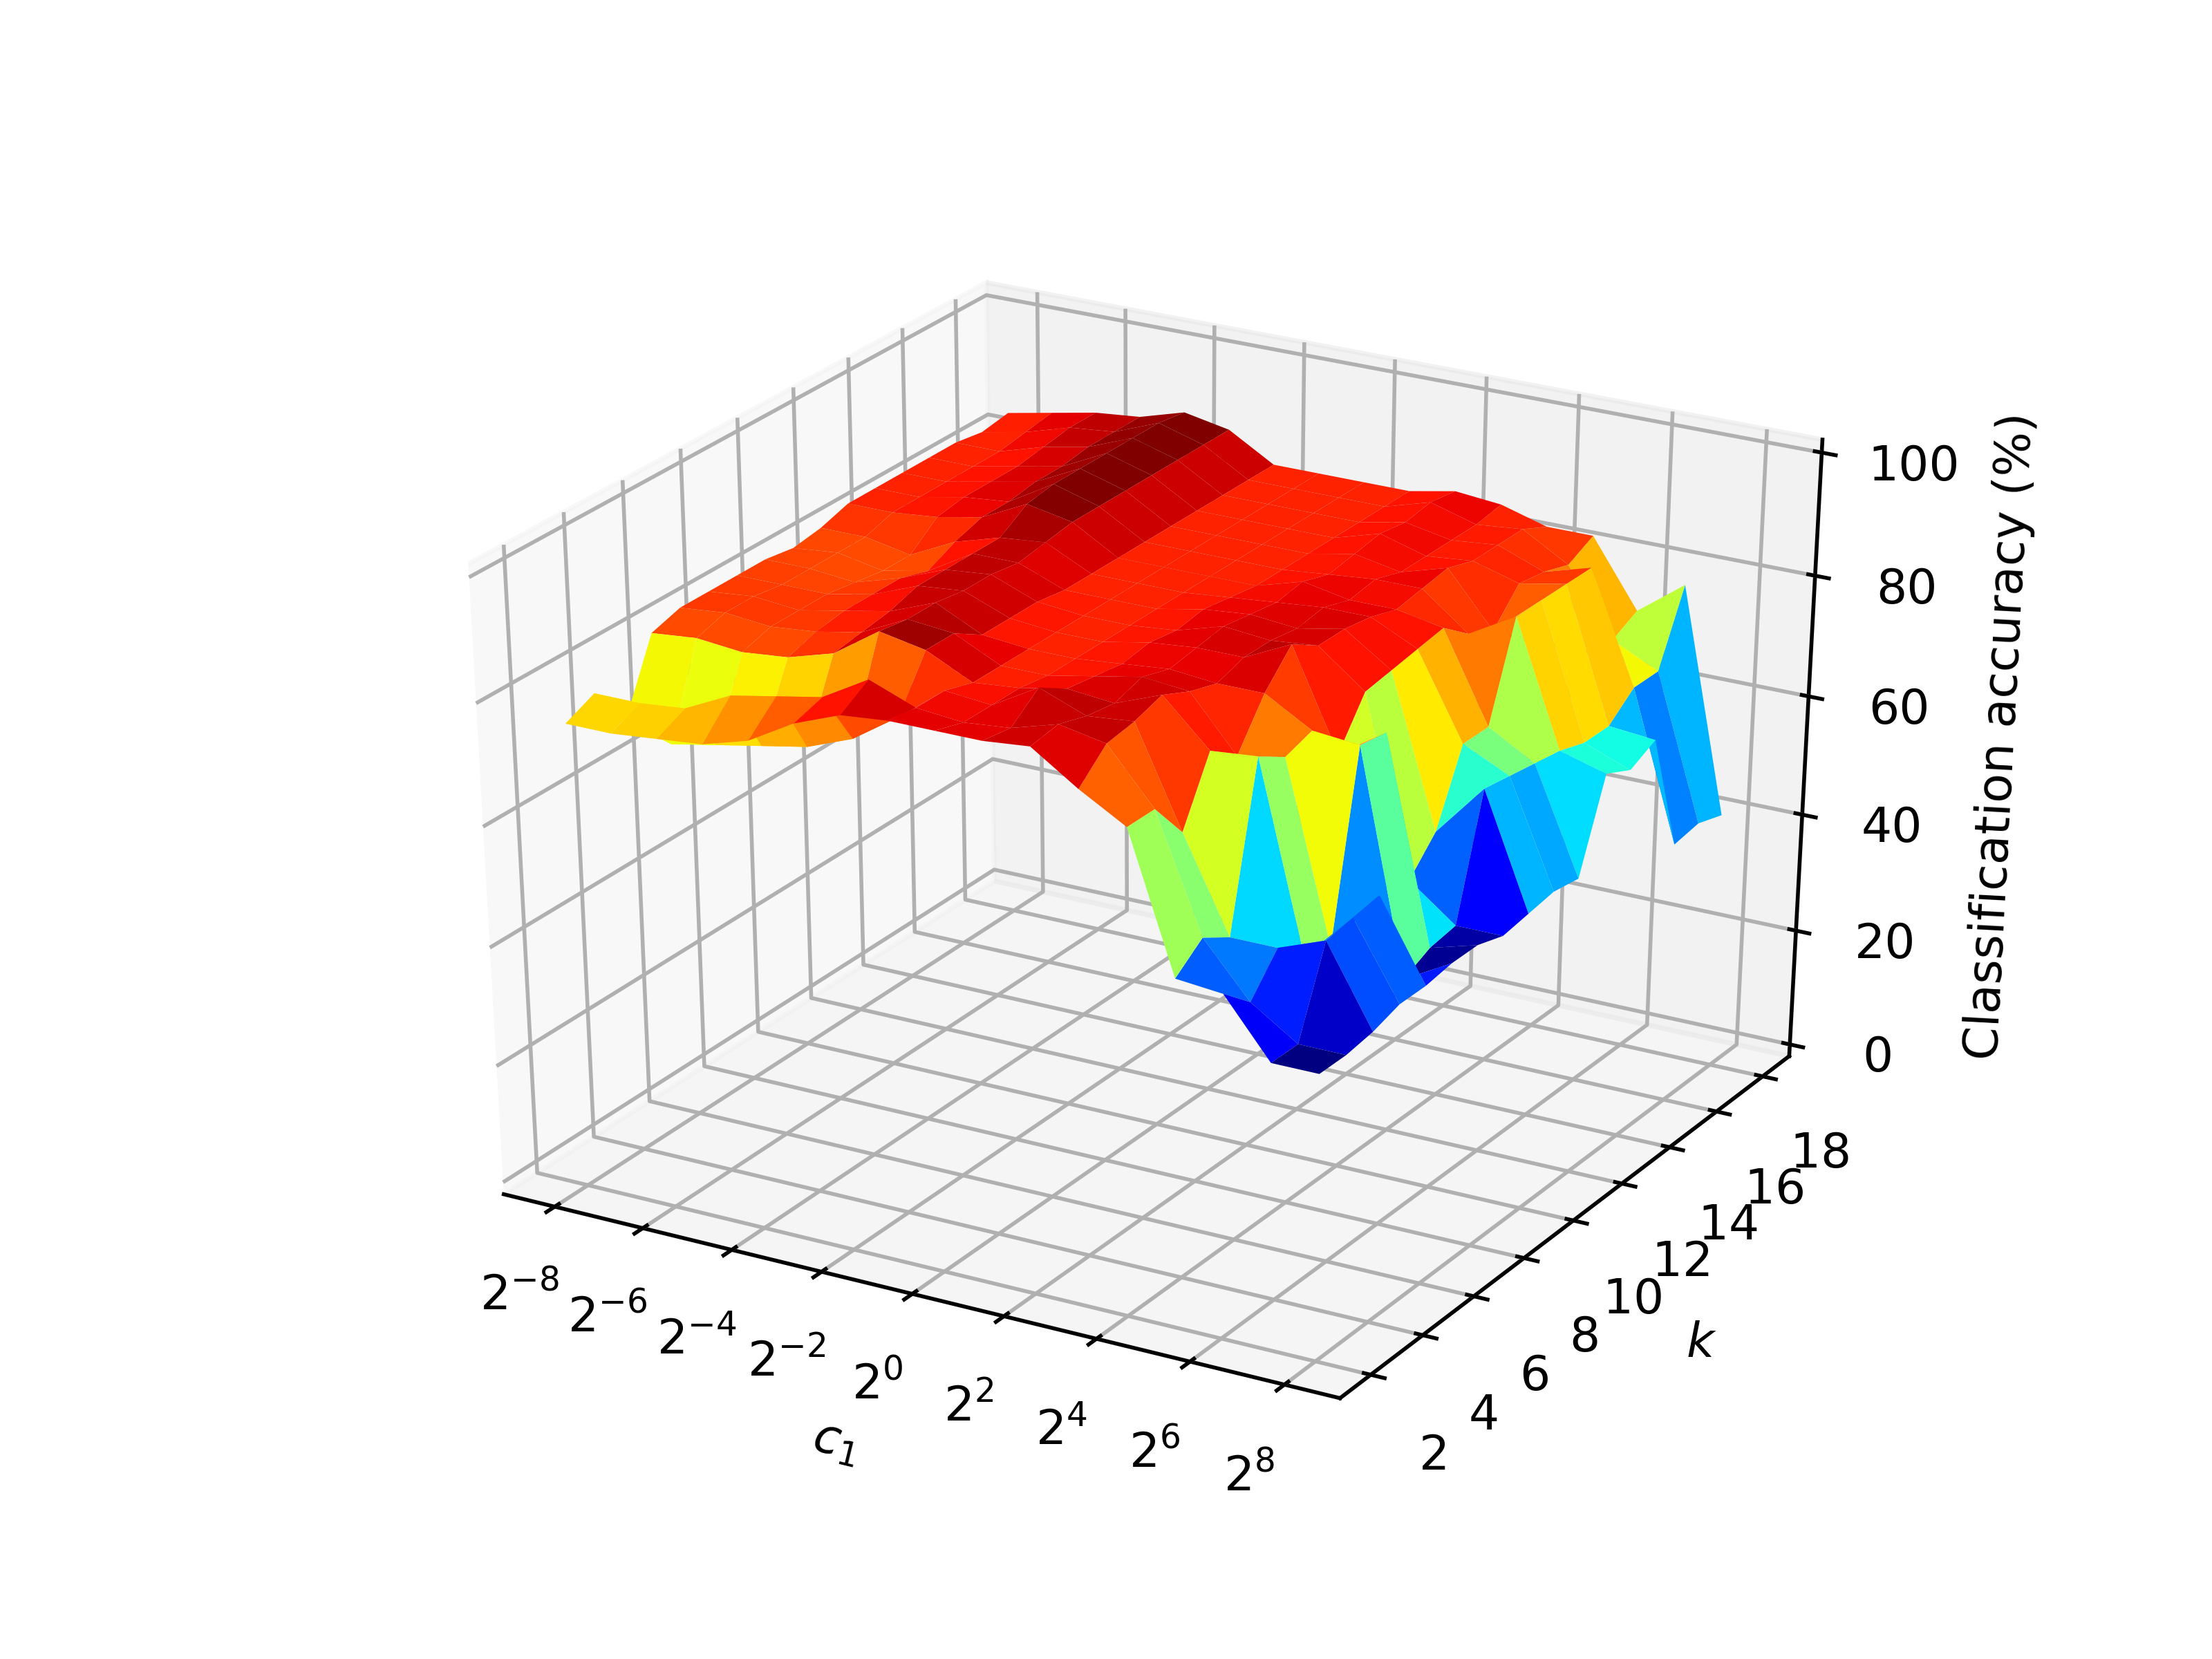
\includegraphics[width=0.5\textwidth]{RKNN-TSVM-Aust-C_1_k}}
	\subfloat[مجموعه داده \lr{Hepatitis}]{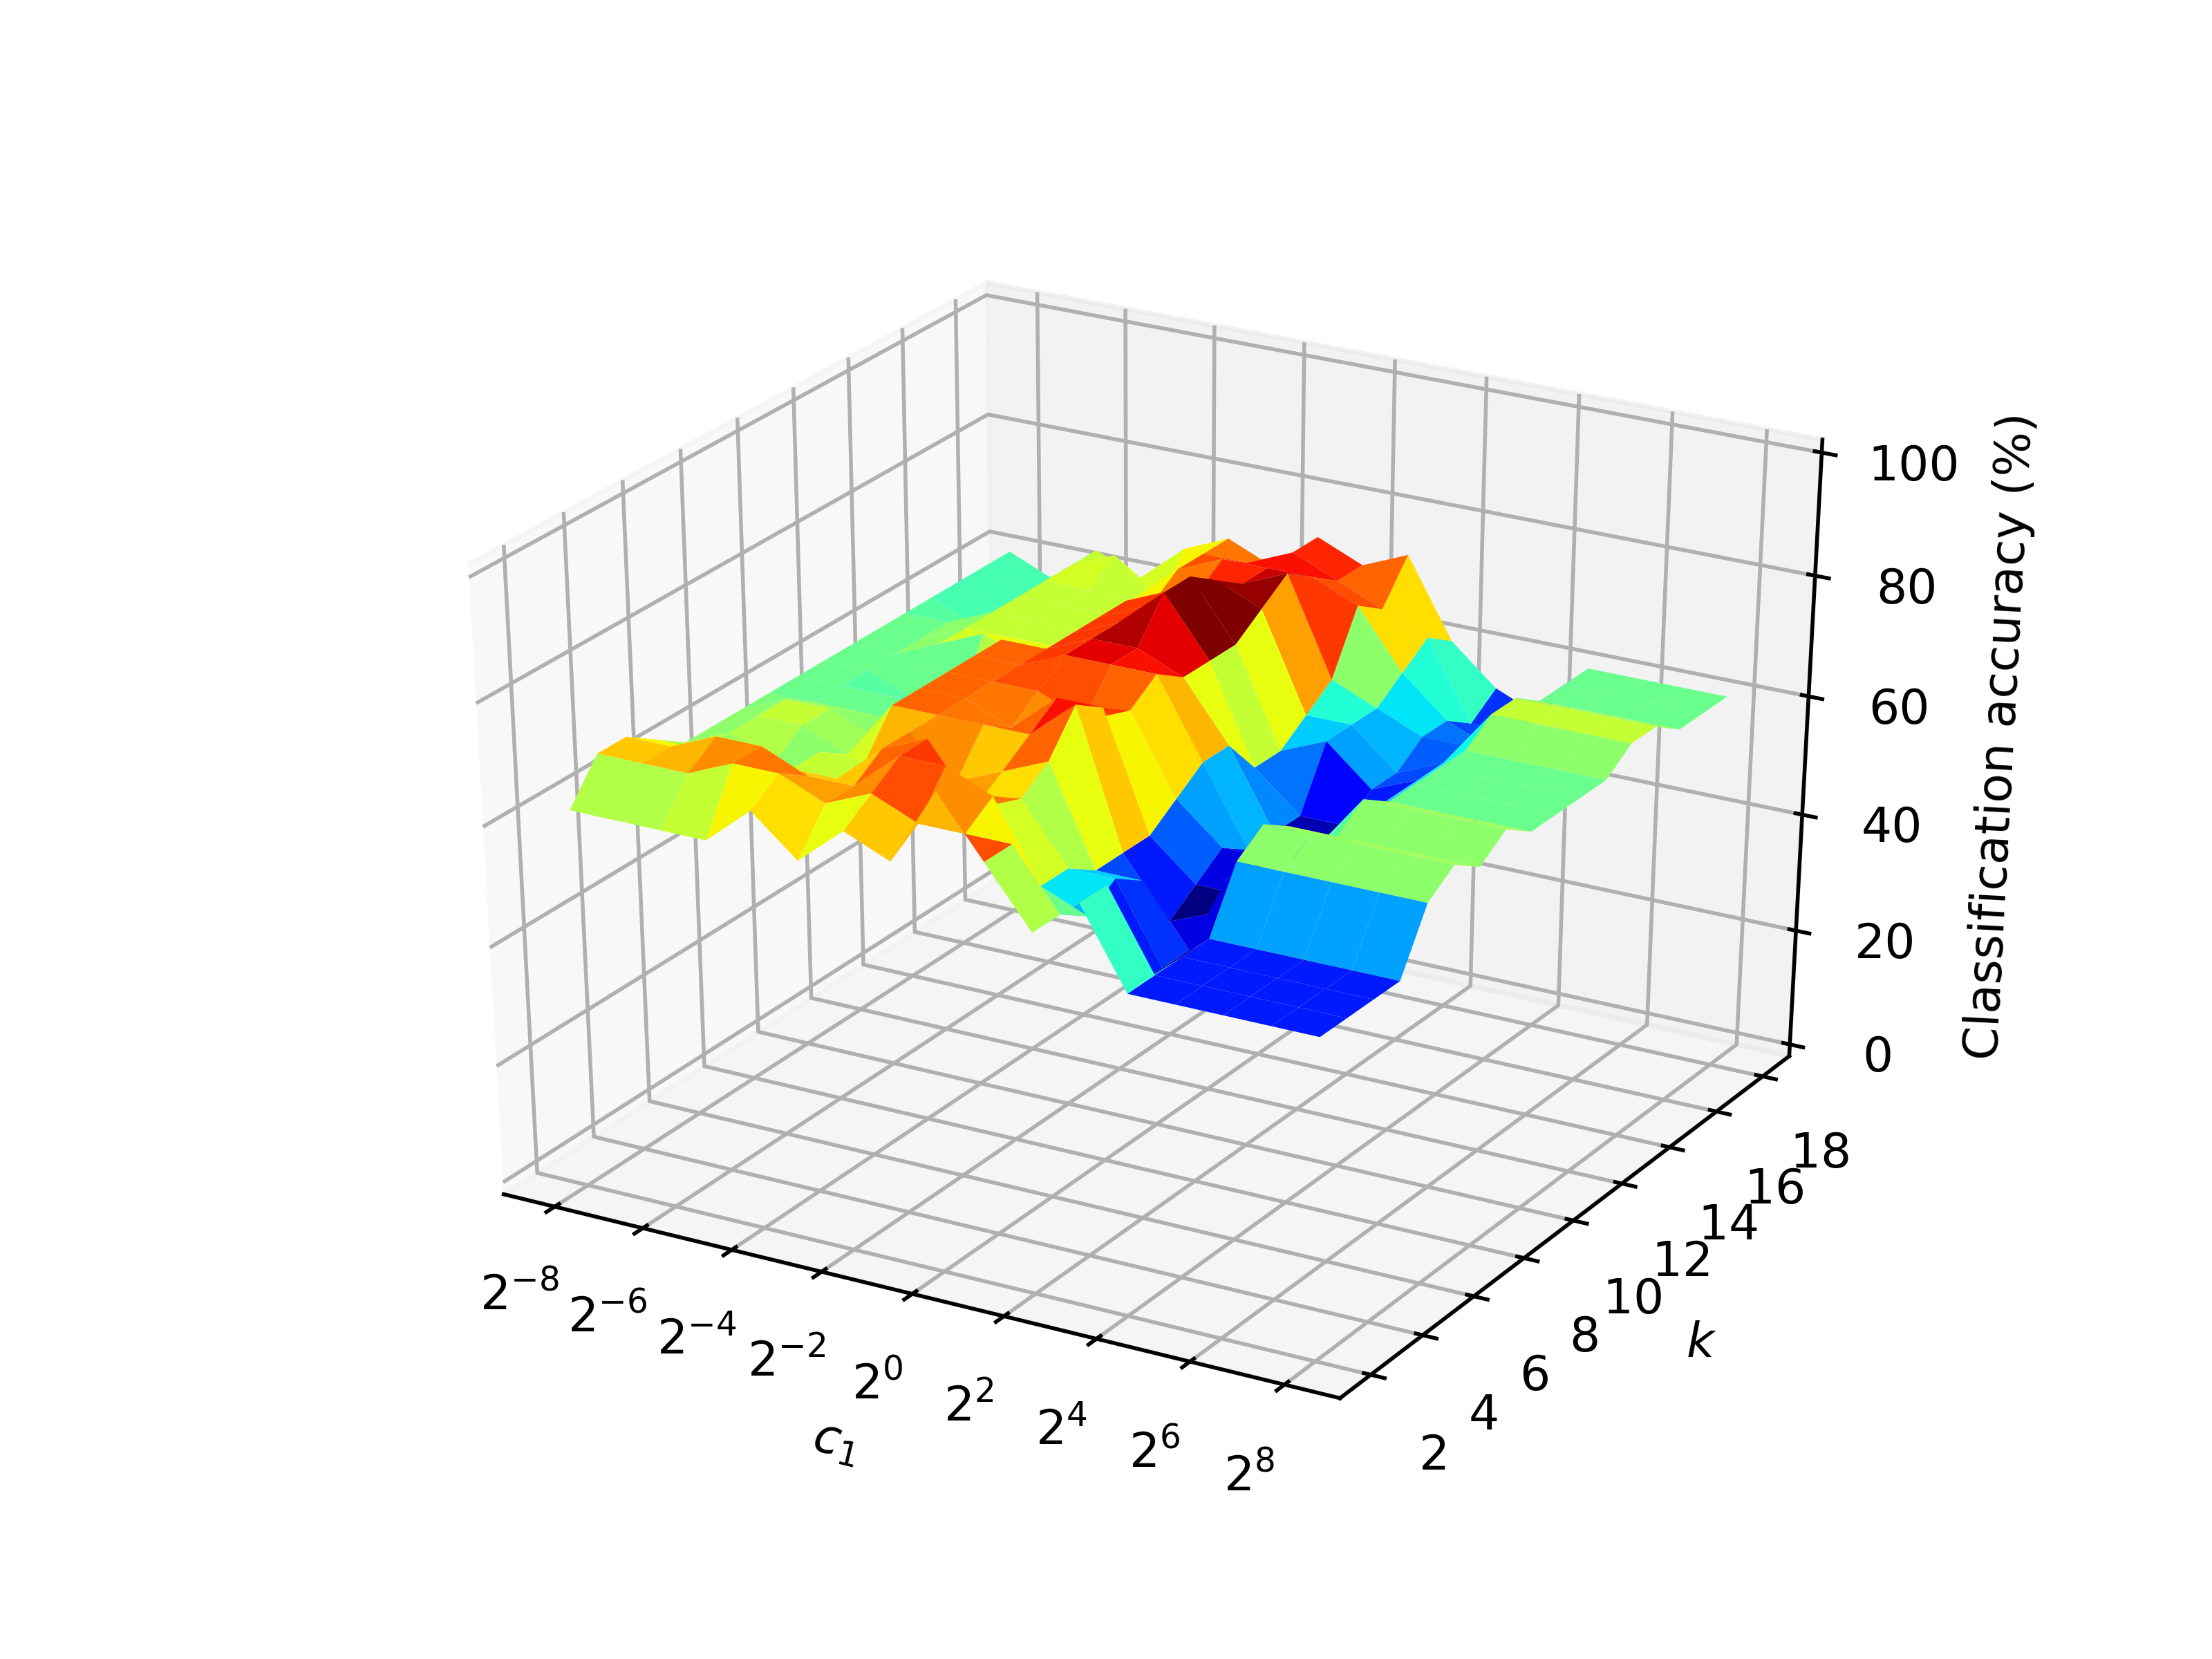
\includegraphics[width=0.5\textwidth]{RKNN-TSVM-Hep-C_1_k}}
	\caption{عملکرد نسخه خطی روش \lr{RKNN-TSVM} روی پارامترهای مختلف $c_{1}$ و $k$}
	\label{fig:RKNN-TSVM-Aust-Hep-C_1_k}
\end{figure}

برای هر مجموعه داده، در این آزمایش، تعداد حالت‌های پارامترهای $c_{1}$ $c_{2}$، و $k$ برابر با 17 است. بطوریکه تعداد ترکیبات $(c_{1},c_{2})$ و $(c_{1}, k)$ مساوی با 289 می‌باشد. شکل \ref{fig:RKNN-TSVM-Aust-Hep-C_1_2} عملکرد نسخه خطی روش روی پارامترهای مختلف $c_{1}$ و $c_{2}$ نشان می‌دهد. همانطور در این شکل نشان داده شده است، مقادیر پارامتر $c_{2}$ دقت دسته‌بندی روش \lr{RKNN-TSVM} را بهبود می‌دهد. بنابراین می‌توان نتیجه گرفت که ریسک ساختاری دقت روش ‍پیشنهادی (\lr{RKNN-TSVM}) را بهتر می‌کند.

شکل \ref{fig:RKNN-TSVM-Aust-Hep-C_1_k} عملکرد نسخه خطی روش \lr{RKNN-TSVM} روی مقادیر پارامترهای $c_{1}$ و $k$ را نشان می‌دهد. همانطور که در این شکل مشخص شده است، عملکرد روش \lr{RKNN-TSVM} به پارامتر $k$ نیز وابسته است. به عنوان مثال، افزایش مقدار پارامتر $k$ منجر به بهبود دقت روش پیشنهادی روی مجموعه داده \lr{Hepatitis} شده است. به طور خلاصه، آزمایش‌های این بخش نشان می‌دهد که دقت روش پیشنهادی (\lr{RKNN-TSVM}) وابسته به انتخاب بهینه پارامترهایش است.

\subsubsection{آزمایش با مجموعه داده \lr{NDC}}\label{sec:5:3:3:5}
به منظور بررسی سرعت آموزش روش \lr{RKNN-TSVM} بر روی مجموعه داده‌های بزرگ، آزمایش بر روی مجموعه داده \lr{NDC} \cite{musicant1998} صورت گرفته است. مشخصات مجموعه داده‌های \lr{NDC} در جدول \ref{tab:5} نشان داده شده است. جهت آزمایش با مجموعه داده \lr{NDC}، پارامتر $C$ برای تمام روش برابر با یک است. در نسخه غیر خطی از تابع \lr{RBF} با پارامتر $\sigma=2^{-15}$ استفاده شده است. همچنین پارامتر  $k$ برای روش‌های \lr{WLTSVM} و \lr{RKNN-TSVM} برابر با 5 است. 

جدول \ref{tab:11} مقایسه زمان آموزش روش‌های \lr{TSVM}،\lr{WLTSVM} و \lr{RKNN-TSVM} با تابع هسته خطی را نشان می‌دهد. مشابه روش \lr{TSVM}، روش \lr{TBSVM} دو مسئله دوگان را برای بدست آوردن مدل خروجی حل می‌کند. بنابراین زمان آموزش روش \lr{TBSVM} در این آزمایش آورده نشده است. ستون آخر نسبت تسریع الگوریتم \lr{LDMDBA} را نشان می‌دهد که به این صورت تعریف می‌شود: 
\begin{align*}
%\small
\textrm{نسبت تسریع} = \frac{\textrm{زمان آموزش روش \lr{RKNN-TSVM(FSA)}}}{\textrm{زمان آموزش روش \lr{RKNN-TSVM(LDMDBA)}}}
\end{align*}

نتایج در جدول \ref{tab:11} نشان می‌دهد که الگوریتم \lr{LDMDBA} سرعت آموزش روش پیشنهادی را به طور قابل توجه‌ای بهبود داده است. بطوریکه با افزایش تعداد نمونه‌های آموزشی، نسبت تسریع الگوریتم \lr{LDMDBA} بیشتر می‌شود. برای مثال، روش پیشنهادی با الگوریتم \lr{LDMDBA} از روش پیشنهادی با الگوریتم \lr{FSA} روی مجموعه داده \lr{NDC-25K} حدود $3.25$ سریع‌تر است. همچنین سرعت آموزش نسخه خطی روش \lr{RKNN-TSVM} با الگوریتم \lr{LDMDBA} بسیار نزدیک به نسخه خطی \lr{TSVM} می‌باشد. بطوریکه نسخه خطی روش پیشنهادی از  نسخه خطی \lr{TSVM} روی مجموعه داده \lr{NDC-50K} کمی سریع‌تر است. زیرا روش پیشنهادی دو مسئله دوگان با اندازه کوچک‌تر حل می‌کند. به عبارت دیگر فقط نمونه‌های حاشیه‌ای در مسئله دوگان نقش دارند.

\begin{table*}[!t]
	\small
	\centering
	\caption{مقایسه زمان آموزش روش \lr{RKNN-TSVM} با سایر روش روی مجموعه داده \lr{NDC} با تابع هسته خطی}
	\ra{1.3} % Space between rows
	\begin{threeparttable}
		\begin{tabular}{l c c c c c}
			\toprule
			% after \\: \hline or \cline{col1-col2} \cline{col3-col4} ...
			مجموعه داده & \lr{TSVM} & \lr{WLTSVM} & \lr{RKNN-TSVM(FSA)} & \lr{RKNN-TSVM(LDMDBA)} & \\
			& زمان اجرا & زمان اجرا & زمان اجرا & زمان اجرا  & نسبت تسریع \\
			\midrule
			%NDC-700 & 0.019 & 0.047 & 0.042 & 0.032 & 1.31\\ 
			%NDC-900 & 0.031 & 0.079 & 0.065 & 0.042 & 1.55\\ 
			\lr{NDC-1K} & $0.064$ & $0.092$ & $0.079$ & $0.052$ & $1.52$\\ 
			\lr{NDC-2K} & $0.12$ & $0.36$ & $0.292$ & $0.19$ & $1.54$\\ 
			\lr{NDC-3K} & $0.26$ & $0.84$ & $0.662$ & $0.295$ & $2.24$\\ 
			\lr{NDC-4K} & $0.422$ & $1.476$ & $1.192$ & $0.562$ & $2.12$ \\
			\lr{NDC-5K} & $0.693$ & $2.397$ & $1.884$ & $0.828$ & $2.28$\\
			\lr{NDC-10K} & $2.556$ & $9.872$ & $7.628$ & $2.727$  & $2.8$ \\
			\lr{NDC-25K} & $17.606$ & $68.893$ & $52.867$ & $16.25$  & $3.25$\\
			\lr{NDC-50K} & $70.1$ & \tnote{\lr{a}} & \tnote{\lr{a}} & $64.433$  & -\\
			\bottomrule
		\end{tabular}
		\begin{tablenotes}
			\item[\lr{a}] آزمایش به دلیل کمبود حافظه خاتمه یافته است.
		\end{tablenotes}
	\end{threeparttable}
	\label{tab:11}
\end{table*}

\begin{table*}[!t]
	\small
	\centering
\caption{مقایسه زمان آموزش روش \lr{RKNN-TSVM} با سایر روش روی مجموعه داده \lr{NDC} با تابع هسته \lr{RBF}}
	\ra{1.3} % Space between rows
	\begin{threeparttable}
		\begin{tabular}{l c c c c c}
			\toprule
			% after \\: \hline or \cline{col1-col2} \cline{col3-col4} ...
			مجموعه داده & \lr{TSVM} & \lr{WLTSVM} & \lr{RKNN-TSVM(FSA)} & \lr{RKNN-TSVM(LDMDBA)} & \\
			& زمان اجرا & زمان اجرا & زمان اجرا & زمان اجرا  & نسبت تسریع\\
			\midrule
			%NDC-700 & 0.102 & 0.315 & 0.309 & 0.273 & 1.13 \\ 
			%NDC-900 & 0.161 & 0.611 & 0.591 & 0.454 & 1.3 \\ 
			\lr{NDC-1K} & $0.203$ & $0.803$ & $0.807$ & $0.555$ & $1.45$\\ 
			\lr{NDC-2K} & $0.983$ & $5.731$ & $5.729$ & $2.442$ & $2.35$\\ 
			\lr{NDC-3K} & $2.74$ & $18.225$ & $18.599$ & $6.465$ & $2.88$\\
			\lr{NDC-4K} & $5.896$ & $42.234$ & $41.784$ & $12.485$ & $3.35$\\ 
			\lr{NDC-5K} & $10.328$ & $84.188$ & $82.507$ & $21.14$ & $3.9$\\
			\lr{NDC-10K}\textsuperscript{\lr{b}} & $4.605$ & $67.626$ & $64.721$ & $8.606$ & $7.52$\\
			\lr{NDC-25K}\textsuperscript{\lr{b}} & $31.459$ & $983.678$ & $963.341$ & $67.485$  & $14.27$\\
			\lr{NDC-50K}\textsuperscript{\lr{b}} & $186.761$ & \tnote{\lr{a}} & \tnote{\lr{a}} & $357.942$  & -\\
			\bottomrule
		\end{tabular}
		\begin{tablenotes}
			\item[\lr{a}]  اجرای روش به دلیل زیاد بودن زمان آزمایش خاتمه یافته است.
			\item[\lr{b}] از تابع هسته مستطیلی با اندازه 10 درصد نمونه‌های آموزشی استفاده شده است.
		\end{tablenotes}
	\end{threeparttable}
	\label{tab:12}
\end{table*}

جدول \ref{tab:12} مقایسه زمان آموزش روش‌های \lr{TSVM}،\lr{WLTSVM} و \lr{RKNN-TSVM} با تابع هسته \lr{RBF} را نشان می‌دهد. نتایج با تابع هسته غیر خطی نشان می‌دهد که روش پیشنهادی با الگوریتم \lr{LDMDBA} از روش \lr{WLTSVM}  و روش \lr{RKNN-TSVM} با الگوریتم  \lr{FSA} بسیار سریع‌تر است. بطوریکه بیشترین نسبت تسریع با الگوریتم \lr{LDMDBA} مساوی با 14 برابر می‌باشد. با وجود اینکه از تابع هسته تقلیل یافته برای مجموعه داده‌های بزرگ از 5 هزار نمونه استفاده شده است،  روش \lr{TSVM} همچنان حدود 2 برابر سریع‌تر از روش پیشنهادی با الگوریتم \lr{LDMDBA} است. زیرا روش پیشنهادی با الگوریتم \lr{LDMDBA} و تابع هسته تقلیل یافته $(n \times \bar{n})$ علاوه بر پیدا کردن نزدیک‌ترین همسایه‌های تمام نمونه‌ها، دو مسئله دوگان نیز حل می‌کند.

نتایج روی مجموعه داده \lr{NDC} با تابع هسته \lr{RBF} این فرضیه را تایید می‌کند که الگوریتم \lr{LDMDBA} برای نسخه غیر خطی روش  \lr{RKNN-TSVM} مناسب است. زمان اجرای این الگوریتم روی داده‌های با ابعاد بالا بسیار بهتر از الگوریتم \lr{FSA} می‌باشد. به طور خلاصه، روش \lr{RKNN-TSVM} با الگوریتم \lr{LDMDBA} نسبت به روش \lr{WLTSVM} روی مجموعه داده‌های بزرگ از نظر زمان اجرا بسیار بهتر عمل می‌کند.

\section{جمع‌بندی}\label{sec:5:4}
در این فصل، دو دسته‌بند پیشنهادی یعنی \lr{KNN-LSTSVM} و \lr{RKNN-TSVM} مورد بررسی و ارزیابی قرار گرفت. روش \lr{KNN-LSTSVM} مزیت‌های اصلی دو روش \lr{WLTSVM} و \lr{LSTSVM} را دارد که عبارتند از:
\begin{enumerate}
	\item مشابه روش \lr{WLTSVM}، اطلاعات شباهت نمونه‌ها را با ساخت گراف نزدیک‌ترین همسایه در مسئله بهینه‌سازی لحاظ می‌کند. بطوریکه به هر نمونه بر اساس شمارش تعداد همسایه‌های نزدیکش وزن داده می‌شود. همچنین نمونه‌های حاشیه‌ای هر کلاس نیز با استفاده از گراف ساخته شده مشخص می‌گردد.  نتایج بر روی مجموعه داده‌های مصنوعی (بخش \ref{sec:5:2:2}) و واقعی (بخش \ref{sec:5:2:3}) نشان می‌دهد دقت مدل خروجی نسبت به روش \lr{LSTSVM} بهبود یافته است .
	\item مشابه روش \lr{LSTSVM}، قید مسئله بهینه‌سازی در تابع هدف جایگذاری می‌شود. بطوریکه مدل خروجی با حل کردن دو دستگاه معادلات خطی بدست می‌آید. در حالی‌که در روش  \lr{WLTSVM} دو مسئله دوگان حل می‌شود. نتایج ارزیابی روی مجموعه داده‌های بزرگ  (بخش \ref{sec:5:2:4}) نشان می‌دهد که سرعت آموزش نسبت به روش \lr{WLTSVM} بسیار افزایش یافته است.    
\end{enumerate}

روش پیشنهادی دوم یعنی \lr{RKNN-TSVM} روش \lr{WLTSVM} را از نظر دقت و سرعت آموزش بهبود داده است:
\begin{enumerate}
	\itemsep0em
	\item \lr{RKNN-TSVM} برخلاف روش  \lr{WLTSVM} به یک نمونه براساس فاصله نزدیک‌ترین همسایه‌هایش از نمونه مورد نظر وزن می‌دهد. همچنین روش پیشنهادی ریسک ساختاری را در مسئله بهینه سازی کمینه می‌کند. نتایج بر روی مجموعه داده‌های مصنوعی  (بخش \ref{sec:5:3:3:1}) و واقعی (بخش  \ref{sec:5:3:3:2}) نشان می‌دهد که دقت دسته‌بندی و تعمیم‌پذیری روش پیشنهادی نسبت به روش \lr{WLTSVM} بهبود یافته است.
	\item محاسبه گراف نزدیک‌ترین همسایه جهت وزن‌دهی به نمونه‌ها، یک چالش در روش پیشنهادی است. به منظور حل کردن این چالش، الگوریتم  \lr{LDMDBA} به منظور سرعت بخشیدن به فرآیند پیدا کردن نزدیک‌ترین همسایه‌های نمونه‌ها استفاده شده است. نتایج بر روی مجموعه داده‌های بزرگ نشان می‌دهد که الگوریتم  \lr{LDMDBA} سرعت آموزش روش پیشنهادی را برای هر دو نسخه خطی و غیر خطی به طور قابل    توجه‌ای افزایش داده است. بطوریکه سرعت یادگیری تا 14 برابر نسبت به روش \lr{WLTSVM} سریع‌تر شده است.
\end{enumerate}

